\documentclass[11pt]{article}

% ------------------------------------------------------------------------------------------------------------------------
% PACKAGES
% Vous pouvez ajouter des packages si besoin
% Éviter les packages trop exotiques ou connus pour poser des problèmes / incompatibilités
% ------------------------------------------------------------------------------------------------------------------------
\usepackage[utf8]{inputenc}
\usepackage[T1]{fontenc}
\usepackage{siunitx}
\usepackage[dvipsnames]{xcolor}
\sisetup{separate-uncertainty,
locale = FR, scientific-notation = false, exponent-product = \times, inter-unit-product = \ensuremath{{}\cdot{}}}
\usepackage{graphicx}
\usepackage{amsmath, amssymb}
\usepackage[version=4]{mhchem} %affichage des formules chimiques
\usepackage{pgfplots} %plots directement dans latex
\pgfplotsset{height = 7cm,width=12cm,compat=1.9}
% \usepgfplotslibrary{external}
%\tikzexternalize
\usetikzlibrary{angles, arrows.meta, quotes,calc}
\usepackage{float}
\floatplacement{figure}{H}%placement par défaut des figures !h!tbp
\usepackage[%
      a4paper,%
      textwidth=16cm,%
      top=2cm,%
      bottom=2cm,%
      headheight=25pt,%
      headsep=12pt,%
      footskip=25pt]{geometry}%
\usepackage[french]{babel}
\parindent0pt

\usepackage{caption}
\captionsetup{
    labelformat=empty,
    width = .93\textwidth
}

\usepackage{hyperref}

% ------------------------------------------------------------------------------------------------------------------------
% MACROS
% Ne rajouter que des macros réellement nécessaires afin de réduire la probabilité de conflit
% ------------------------------------------------------------------------------------------------------------------------
% Ensembles mathématiques
\def		\K	{	\ensuremath	{\mathbb	{K}	}	}
\def		\N	{	\ensuremath	{\mathbb	{N}	}	}
\def		\NN	{	\ensuremath	{\mathbb	{N}	}	}
\def		\Z	{	\ensuremath	{\mathbb	{Z}	}	}
\def		\Q	{	\ensuremath	{\mathbb	{Q}	}	}
\def		\R	{	\ensuremath	{\mathbb	{R}	}	}
\def		\RR	{	\ensuremath	{\mathbb	{R}	}	}
\def		\C	{	\ensuremath	{\mathbb	{C}	}	}

% Guillemets français et anglais (simples et doubles)
\newcommand{\frquotes}[1]{\og{#1}\fg}
\newcommand{\ensquotes}[1]{`{#1}'}
\newcommand{\enquotes}[1]{``{#1}''}

% Valeurs absolues
\newcommand{\abs}[1]{\ensuremath{\left|{#1}\right|}}

% ------------------------------------------------------------------------------------------------------------------------
% OPÉRATEURS
% ------------------------------------------------------------------------------------------------------------------------
\DeclareMathOperator{\cotan}{cotan}


% ------------------------------------------------------------------------------------------------------------------------
\newcounter{qNum}

\newif\ifdraft
% Le booléen suivant définit si on est en mode draft (avec affichage des réponses vraies/fausses et méta-données) ou production (cases)
% Commenter pour le mode production ; dé-commenter la ligne \draftrue dans le headers.tex pour voir les détails
\drafttrue

\ifdraft
    \newenvironment{question}[4]
    	{\noindent\rule{\textwidth}{0.5pt}\\{\bf Question~:} \refstepcounter{qNum}\theqNum \par{\bf SF~:} #1 \par{\bf Thème~:} #2 \par{\bf Niveau~:} #3 \par{\bf Dépendance~:} #4 \par\noindent\rule{\textwidth}{0.25pt}\\}
    	{ }
    
    \newenvironment{reponses}
    	{\begin{description}}
    	{\end{description}}
\else
    \newenvironment{question}[4]
    	{\refstepcounter{qNum} \subsubsection{ Question \theqNum} \noindent\rule{.5\textwidth}{0.25pt}\\ {\bf SF~:} #1 \par{\bf Thème~:} #2\par{\bf Niveau~:} #3 \par{\bf Dépendance~:} #4 \par \noindent\rule{.5\textwidth}{0.25pt}\\}
    	{ }

    
    \newenvironment{reponses}
    	{\renewcommand{\descriptionlabel}[1]{$\square$} \begin{description}  }
    	{\end{description}}

\fi


\begin{document}
\tableofcontents

\section{Trigonométrie}
	
		\subsection{Utiliser les formules trigo pour trouver une longueur ou un angle dans un triangle rectangle}
        
        	\begin{question}{1217}{Trigonométrie}{1}{/}
				Dans un triangle rectangle, on cherche la relation qui relie un angle (différent de l'angle droit) avec les longueurs du côté adjacent à l'angle et de l'hypoténuse (le grand côté). A quoi est égal $\frac{adjacent}{hypotenuse}$?
            \end{question}

            \begin{reponses}
            	\item[false] $\sin(angle)$
            	\item[false] $\tan(angle)$
                \item[true] $\cos(angle)$
                \item[false] $angle$
            \end{reponses}
			%%%%%%%%%%%%%%%%%%%%%%%%%%%%%%%%%%%%%
        
        	\begin{question}{1217}{Trigonométrie}{1}{/}
				Dans un triangle rectangle, on cherche la relation qui relie un angle (différent de l'angle droit) avec les longueurs du côté opposé à l'angle et de l'hypoténuse (le grand côté). A quoi est égal $\frac{oppose}{hypotenuse}$?
            \end{question}

            \begin{reponses}
            	\item[true] $\sin(angle)$
            	\item[false] $\tan(angle)$
                \item[false] $\cos(angle)$
                \item[false] $angle$
            \end{reponses}
			%%%%%%%%%%%%%%%%%%%%%%%%%%%%%%%%%%%%%
        
        	\begin{question}{1217}{Trigonométrie}{1}{/}
				Dans un triangle rectangle, on cherche la relation qui relie un angle (différent de l'angle droit) avec les longueurs du côté adjacent à l'angle et du côté opposé à l'angle. A quoi est égal $\frac{oppose}{adjacent}$?
            \end{question}

            \begin{reponses}
            	\item[false] $\sin(angle)$
                \item[true] $\tan(angle)$
                \item[false] $\cos(angle)$
            	\item[false] $angle$
            \end{reponses}
			%%%%%%%%%%%%%%%%%%%%%%%%%%%%%%%%%%%%
        
        	\begin{question}{1217}{Trigonométrie}{1}{/}
				Dans un triangle rectangle, on cherche la relation qui relie un angle $\alpha$ (différent de l'angle droit) avec les longueurs du côté adjacent $AB$ à l'angle et de l'hypoténuse $AC$ (le grand côté). A quoi est égal $\frac{AB}{AC}$?
            \end{question}

            \begin{reponses}
            	\item[false] $\sin(\alpha)$
            	\item[false] $\tan(\alpha)$
                \item[true] $\cos(\alpha)$
                \item[false] $\alpha$
            \end{reponses}
			%%%%%%%%%%%%%%%%%%%%%%%%%%%%%%%%%%%%%
        
        	\begin{question}{1217}{Trigonométrie}{1}{/}
				Dans un triangle rectangle, on cherche la relation qui relie un angle $\alpha$ (différent de l'angle droit) avec les longueurs du côté $AB$ opposé à l'angle et de l'hypoténuse $AC$ (le grand côté). A quoi est égal $\frac{AB}{AC}$?
            \end{question}

            \begin{reponses}
            	\item[true] $\sin(\alpha)$
            	\item[false] $\tan(\alpha)$
                \item[false] $\cos(\alpha)$
                \item[false] $\alpha$
            \end{reponses}
			%%%%%%%%%%%%%%%%%%%%%%%%%%%%%%%%%%%%%
        
        	\begin{question}{1217}{Trigonométrie}{1}{/}
				Dans un triangle rectangle, on cherche la relation qui relie un angle $\alpha$ (différent de l'angle droit) avec les longueurs du côté $AB$ adjacent à l'angle et du côté $BC$ opposé à l'angle. A quoi est égal $\frac{BC}{AB}$?
            \end{question}

            \begin{reponses}
            	\item[false] $\sin(\alpha)$
                \item[true] $\tan(\alpha)$
                \item[false] $\cos(\alpha)$
            	\item[false] $\alpha$
            \end{reponses}
			%%%%%%%%%%%%%%%%%%%%%%%%%%%%%%%%%%%%

            \begin{question}{1217}{Trigonométrie}{2}{/}
                Que vaut l'angle $\hat{BAC}$?
                \begin{center}
                	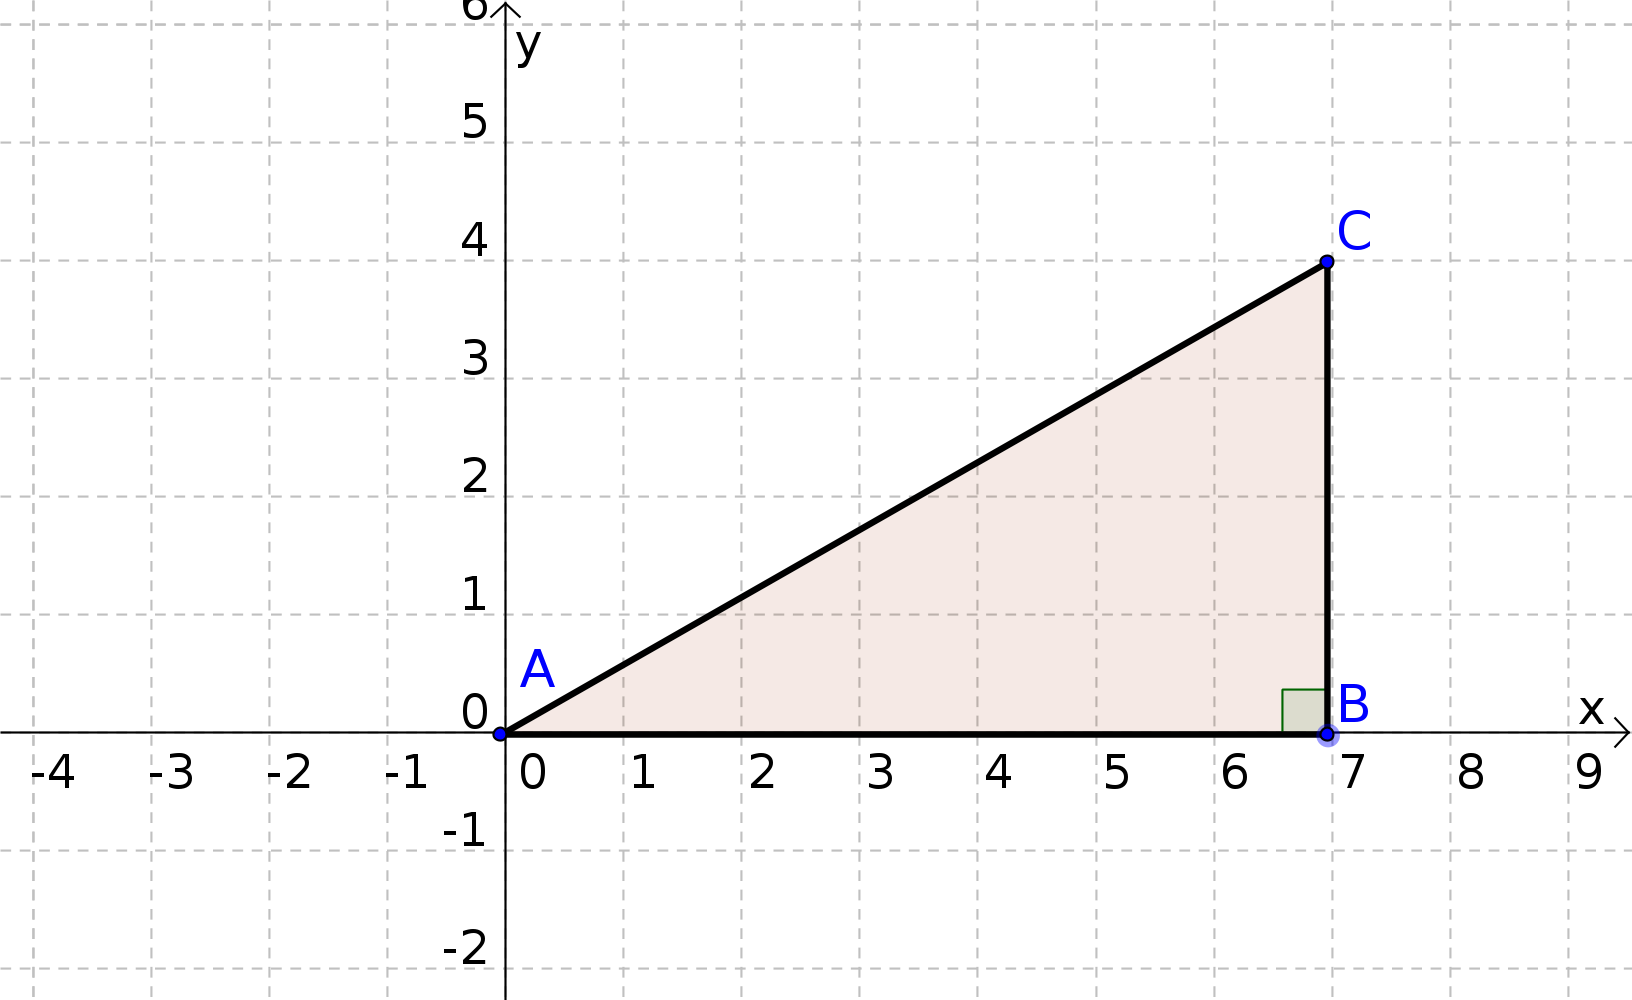
\includegraphics[width=0.5\textwidth]{Philippe/Figures_Philippe/trigo_1_1.png}
                \end{center}
            \end{question}

            \begin{reponses}
                \item[false] $\sin(4/7)$
                \item[true] $\arctan(4/7)$
                \item[false] $\tan(4/7)$
                \item[false] $\arcsin(4/7)$
            \end{reponses}
            %%%%%%%%%%%%%%%%%%%%%%%%%%%%%%%%%%%%%
        
		\subsection{Connaître les formules basiques d’addition des cosinus et sinus}
        
        	\begin{question}{47}{Trigonométrie}{1}{/}
				Soient $\alpha$ et $\beta$ deux angles quelconques. Quelle est l'expression de $\sin(\alpha+\beta)$?
            \end{question}

            \begin{reponses}
            	\item[false] $\cos(\alpha)\cos(\beta)+\sin(\alpha)\sin(\beta)$
            	\item[true] $\sin(\alpha)\cos(\beta)+\cos(\alpha)\sin(\beta)$
                \item[false] $\cos(\alpha)\cos(\beta)-\sin(\alpha)\sin(\beta)$
                \item[false] $\sin(\alpha)\cos(\beta)-\sin(\alpha)\sin(\beta)$
            \end{reponses}
			%%%%%%%%%%%%%%%%%%%%%%%%%%%%%%%%%%%%%
        
        	\begin{question}{47}{Trigonométrie}{1}{/}
				Soient $\alpha$ et $\beta$ deux angles quelconques. Quelle est l'expression de $\cos(\alpha+\beta)$?
            \end{question}

            \begin{reponses}
            	\item[false] $\cos(\alpha)\cos(\beta)+\sin(\alpha)\sin(\beta)$
            	\item[false] $\sin(\alpha)\cos(\beta)+\cos(\alpha)\sin(\beta)$
                \item[true] $\cos(\alpha)\cos(\beta)-\sin(\alpha)\sin(\beta)$
                \item[false] $\sin(\alpha)\cos(\beta)-\sin(\alpha)\sin(\beta)$
            \end{reponses}
			%%%%%%%%%%%%%%%%%%%%%%%%%%%%%%%%%%%%%

            \begin{question}{47}{Trigonométrie}{2}{/}
            	Que vaut $\cos(2\alpha)$ (deux réponses attendues)?
            \end{question}

            \begin{reponses}
                \item[true] $\cos(\alpha)^2-\sin(\alpha)^2$
                \item[false] $\cos(\alpha)^2+\sin(\alpha)^2$
                \item[true] $1-2\sin(\alpha)^2$
                \item[false] $2\sin(\alpha)\cos(\alpha)$
            \end{reponses}
            %%%%%%%%%%%%%%%%%%%%%%%%%%%%%%%%%%%%%

            \begin{question}{47}{Trigonométrie}{3}{/}
            	Que vaut $\sin(\alpha)\cos(\alpha)$?
            \end{question}

            \begin{reponses}
                \item[true] $\sin(2\alpha)/2$
                \item[false] $2\sin(\alpha)$
                \item[false] $\cos(2\alpha)$
                \item[false] $2\cos(\alpha)$
            \end{reponses}
            %%%%%%%%%%%%%%%%%%%%%%%%%%%%%%%%%%%%%

            \begin{question}{47}{Trigonométrie}{3}{/}
            	Que vaut $1-2\cos(\alpha)^2$?
            \end{question}

            \begin{reponses}
                \item[true] $-\cos(2\alpha)$
                \item[false] $2\sin(\alpha)$
                \item[false] $\cos(2\alpha)$
                \item[false] $2\cos(\alpha)$
            \end{reponses}
            %%%%%%%%%%%%%%%%%%%%%%%%%%%%%%%%%%%%%
    
		\subsection{Connaître les valeurs particulières des fonctions trigo}
        
        	\begin{question}{31}{Trigonométrie}{1}{/}
				Quel est le sinus de $0$?
            \end{question}

            \begin{reponses}
            	\item[false] $\frac{\sqrt{2}}{2}$
            	\item[false] 1
                \item[false] $1/2$
                \item[true] 0
            \end{reponses}
			%%%%%%%%%%%%%%%%%%%%%%%%%%%%%%%%%%%%%

            \begin{question}{31}{Trigonométrie}{2}{/}
                Que vaut le cosinus de l'angle représenté ci-dessous?
                \begin{center}
                	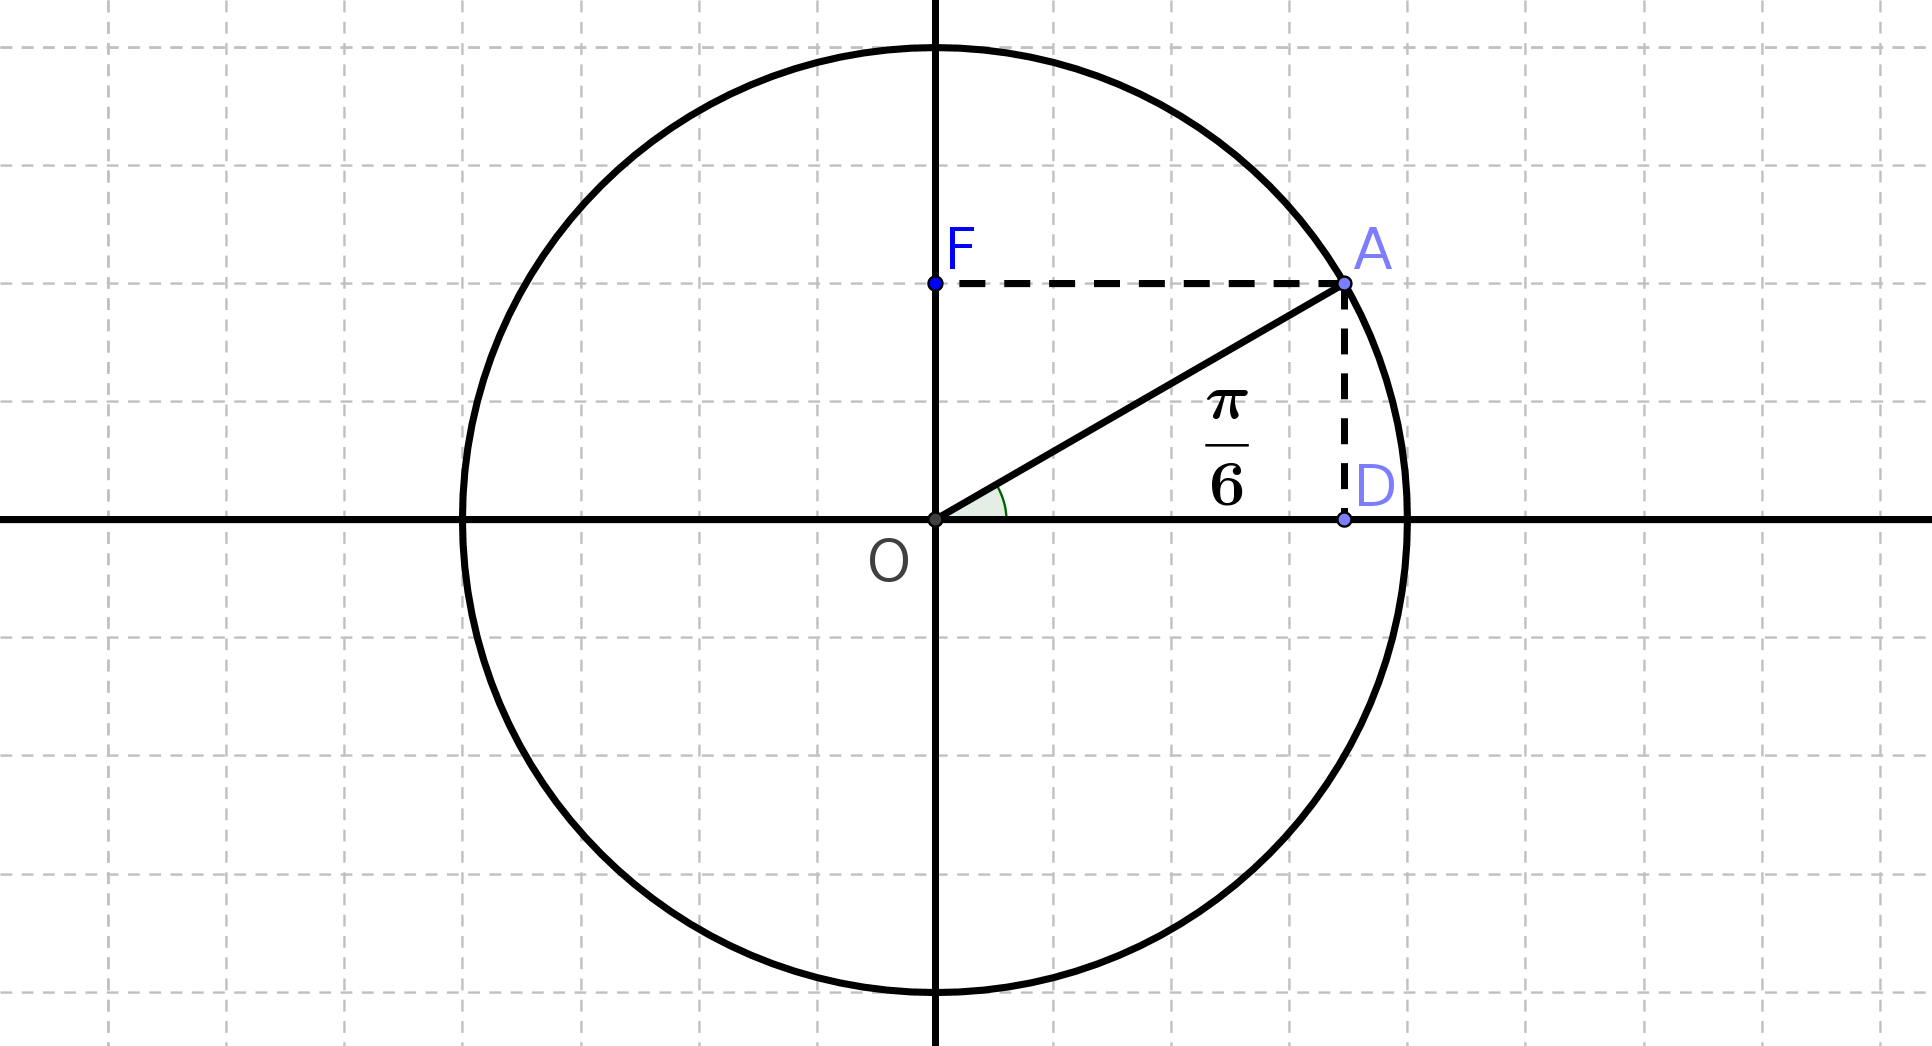
\includegraphics[width=0.5\textwidth]{Philippe/Figures_Philippe/trigo_1_3.png}
                \end{center}
            \end{question}

            \begin{reponses}
                \item[false] $\frac{\sqrt{2}}{2}$
                \item[false] $-\frac{\sqrt{2}}{2}$
                \item[false] $\frac{1}{2}$
                \item[true] $\frac{\sqrt{3}}{2}$
            \end{reponses}
            %%%%%%%%%%%%%%%%%%%%%%%%%%%%%%%%%%%%%
    
            \begin{question}{31}{Trigonométrie}{2}{/}
				Parmi les angles ci-dessous, lequel a pour cosinus $\frac{\sqrt{3}}{2}$?
            \end{question}

            \begin{reponses}
            	\item[false] $\frac{\pi}{3}$
            	\item[true] $\frac{\pi}{6}$
                \item[false] $\frac{\pi}{4}$
                \item[false] $\pi$
            \end{reponses}
            %%%%%%%%%%%%%%%%%%%%%%%%%%%%%%%%%%%%%

            \begin{question}{31}{Trigonométrie}{2}{/}
            	Quel est le sinus de $\frac{\pi}{6}$? 
            \end{question}

            \begin{reponses}
                \item[true] $1/2$
                \item[false] $-1/2$
                \item[false] 1
                \item[false] -1
            \end{reponses}
            %%%%%%%%%%%%%%%%%%%%%%%%%%%%%%%%%%%%%
        
        	\begin{question}{31}{Trigonométrie}{3}{/}
				L'aiguille des heures forme un certain angle avec l'horizontal (0 quand il est 3 heures, $+\frac{\pi}{2}$ quand il est midi). Quel est le cosinus de l'angle ainsi formé quand il est 1 heure? 
            \end{question}

            \begin{reponses}
            	\item[false] $\frac{\sqrt{3}}{2}$
            	\item[false] $-1/2$
                \item[false] $\frac{\sqrt{2}}{2}$
                \item[true] $1/2$
            \end{reponses}
			%%%%%%%%%%%%%%%%%%%%%%%%%%%%%%%%%%%%%
        
        	\begin{question}{31}{Trigonométrie}{3}{/}
				La vitesse d'un objet fait un angle de $-\frac{\pi}{4}$ avec l'axe des $x$. Quel est le sinus de cet angle?
            \end{question}

            \begin{reponses}
            	\item[false] $\frac{\sqrt{3}}{2}$
            	\item[false] $\frac{\sqrt{2}}{2}$
                \item[false] $-\frac{\sqrt{3}}{2}$
                \item[true] $-\frac{\sqrt{2}}{2}$
            \end{reponses}
			%%%%%%%%%%%%%%%%%%%%%%%%%%%%%%%%%%%%%
    
		\subsection{Savoir placer des angles et leurs projections ($\cos$, $\sin$) sur un cercle trigonométrique}
        
        	\begin{question}{1200}{Trigonométrie}{1}{31}
				Quel est le sinus de $\frac{2\pi}{3}$?
            \end{question}

            \begin{reponses}
            	\item[true] $\frac{\sqrt{3}}{2}$
            	\item[false] $\frac{\sqrt{2}}{2}$
                \item[false] 1
                \item[false] $1/2$
            \end{reponses}
			%%%%%%%%%%%%%%%%%%%%%%%%%%%%%%%%%%%%%

            \begin{question}{1200}{Trigonométrie}{2}{31}
                Que valent le cosinus et le sinus de l'angle représenté ci-dessous?
                \begin{center}
                	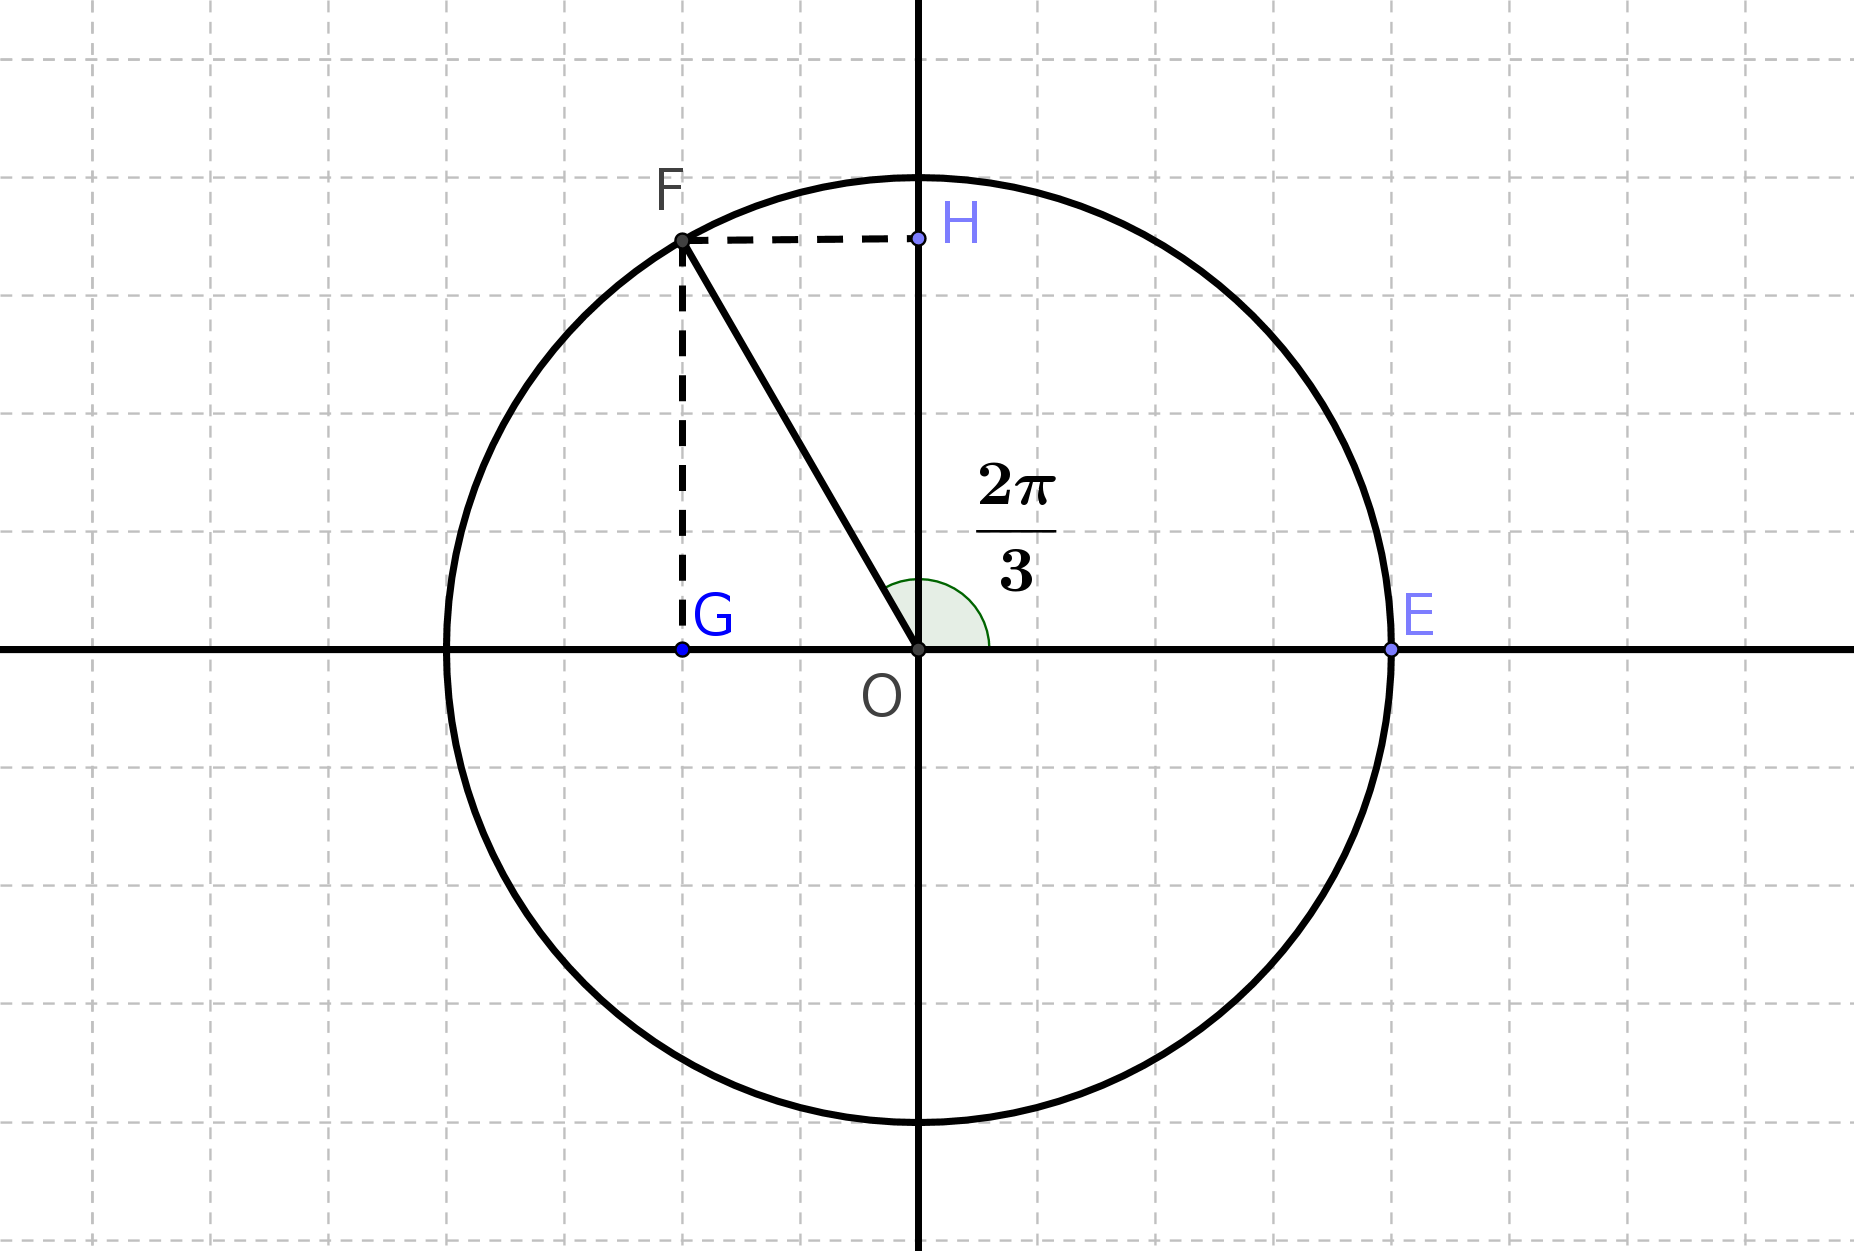
\includegraphics[width=0.5\textwidth]{Philippe/Figures_Philippe/trigo_1_4.png}
                \end{center}
            \end{question}

            \begin{reponses}
                \item[true] $\cos = -\frac{1}{2}$ et $\sin = \frac{\sqrt{3}}{2}$
                \item[false] $\cos = \frac{1}{2}$ et $\sin = \frac{\sqrt{3}}{2}$
                \item[false] $\cos = \frac{\sqrt{3}}{2}$ et $\sin = \frac{1}{2}$
                \item[false] $\cos = -\frac{\sqrt{3}}{2}$ et $\sin = \frac{1}{2}$
            \end{reponses}
            %%%%%%%%%%%%%%%%%%%%%%%%%%%%%%%%%%%%%
        
        	\begin{question}{1200}{Trigonométrie}{2}{31}
				Parmi ces angles, lequel a pour sinus $0,5$?
            \end{question}

            \begin{reponses}
            	\item[false] $\frac{2\pi}{3}$
            	\item[false] $\frac{3\pi}{4}$
                \item[true] $\frac{5\pi}{6}$
                \item[false] $\pi$
            \end{reponses}
			%%%%%%%%%%%%%%%%%%%%%%%%%%%%%%%%%%%%%
        
        	\begin{question}{1200}{Trigonométrie}{2}{31}
				Une force fait un angle $\theta$ avec la verticale. Cet angle a pour cosinus $\frac{\sqrt{2}}{2}$. Parmi les angles suivants, duquel s'agit-il?
            \end{question}

            \begin{reponses}
            	\item[true] $-\frac{\pi}{4}$
            	\item[false] $\frac{3\pi}{4}$
                \item[false] $\frac{5\pi}{4}$
                \item[false] $-\frac{3\pi}{4}$
            \end{reponses}
			%%%%%%%%%%%%%%%%%%%%%%%%%%%%%%%%%%%%%
    
            \begin{question}{1200}{Trigonométrie}{3}{31}
                Parmi ces angles, lequel a pour sinus $-0,5$?
            \end{question}

            \begin{reponses}
                \item[false] $\frac{4\pi}{3}$
                \item[true] $\frac{11\pi}{6}$
                \item[false] $\frac{5\pi}{3}$
                \item[false] $\frac{9\pi}{6}$
            \end{reponses}
            %%%%%%%%%%%%%%%%%%%%%%%%%%%%%%%%%%%%%

            \begin{question}{1200}{Trigonométrie}{3}{31}
                L'angle entre l'aiguille des heures et l'horizontale est de $+\frac{5\pi}{3}$ (dans le sens trigonométrique). Parmi les heures suivantes, de laquelle peut-il s'agir?
            \end{question}

            \begin{reponses}
                \item[false] \SI{7}{\hour}
                \item[false] \SI{3}{\hour}
                \item[true] \SI{5}{\hour} 
                \item[false] \SI{4}{\hour}
            \end{reponses}
            %%%%%%%%%%%%%%%%%%%%%%%%%%%%%%%%%%%%%
	
		\subsection{Utiliser les formules trigo pour trouver une longueur ou un angle dans un triangle rectangle + Manipuler des valeurs d'angles dans des calculs (choisir degré-radian) + Connaître les valeurs particulières des fonctions trigo}

			\begin{question}{/}{Trigonométrie}{2}{1217 et 31 et 1213}
				Un vecteur fait un angle de 60 degrés avec l'axe $x$, et a une norme de 6. Quelle est la composante selon $x$ du vecteur?
            \end{question}

            \begin{reponses}
            	\item[false] $3\sqrt{2}$
            	\item[false] 6
                \item[false] $3\sqrt{3}$
                \item[true] 3
            \end{reponses}
			%%%%%%%%%%%%%%%%%%%%%%%%%%%%%%%%%%%%%

            \begin{question}{/}{Trigonométrie}{2}{1217 et 31 et 1213}
                Que valent les coordonnées $x$ et $y$ du vecteur ci-dessous?
                \begin{center}
                	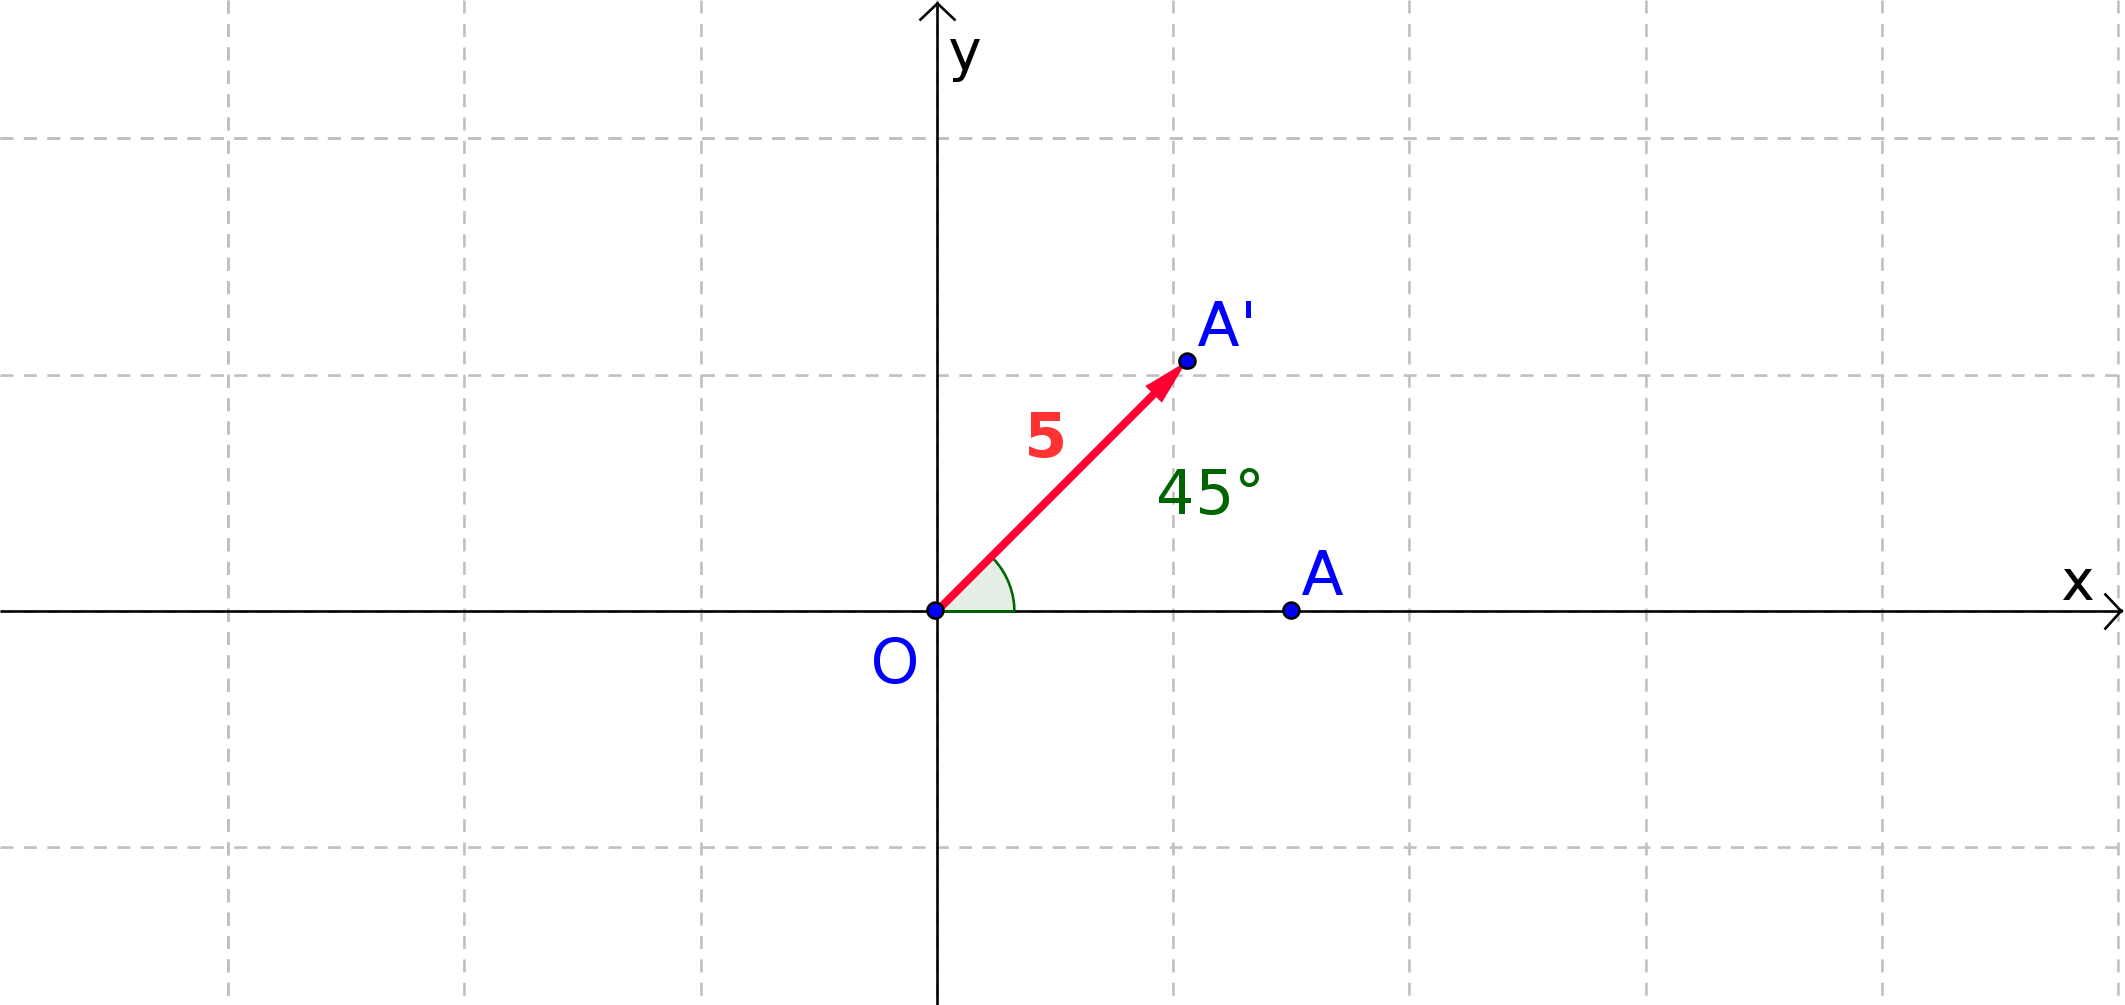
\includegraphics[width=0.5\textwidth]{Philippe/Figures_Philippe/trigo_1_5.png}
                \end{center}
            \end{question}

            \begin{reponses}
                \item[false] $x = \frac{\sqrt{2}}{2}$ et $y = \frac{\sqrt{3}}{2}$
                \item[true] $x = 5\frac{\sqrt{2}}{2}$ et $y = 5\frac{\sqrt{2}}{2}$
                \item[false] $x = 5\frac{\sqrt{3}}{2}$ et $y = \frac{5}{2}$
                \item[false] $x = \frac{\sqrt{3}}{2}$ et $y = \frac{1}{2}$
            \end{reponses}
            %%%%%%%%%%%%%%%%%%%%%%%%%%%%%%%%%%%%%

            \begin{question}{/}{Trigonométrie}{2}{1217 et 31 et 1213}
            	Un objet se déplace avec un angle de 30 degrés par rapport à l'axe horizontal à une vitesse de \SI{10}{\meter\per\second}. Quelle est la valeur de la vitesse de l'objet par rapport à l'axe horizontal?
            \end{question}

            \begin{reponses}
                \item[false] $5\;\si{\meter\per\second}$
                \item[false] $\sqrt{2}/2\;\si{\meter\per\second}$
                \item[false] $\sqrt{3}/2\;\si{\meter\per\second}$
                \item[true] $5\sqrt{3}\;\si{\meter\per\second}$
            \end{reponses}
            %%%%%%%%%%%%%%%%%%%%%%%%%%%%%%%%%%%%%
        
        	\begin{question}{/}{Trigonométrie}{3}{1217 et 31 et 1213}
				Un vecteur de norme $3$ fait un angle $\theta$ avec l'horizontale. La projection sur l'axe vertical est de $1,5$. Parmis les angles suivant, lequel peut être égal à $\theta$?
            \end{question}

            \begin{reponses}
            	\item[false] $\frac{\pi}{2}$
            	\item[false] $\frac{\pi}{3}$
                \item[false] $\frac{\pi}{4}$
                \item[true] $\frac{\pi}{6}$
            \end{reponses}
			%%%%%%%%%%%%%%%%%%%%%%%%%%%%%%%%%%%%%

            \begin{question}{/}{Trigonométrie}{3}{1217 et 31 et 1213}
                Un pendule de longueur \SI{10}{\centi\meter} forme un angle $\theta$ avec la verticale, de manière à ce que sa projection sur l'axe vertical soit de \SI{5}{\centi\meter}. Que vaut $\theta$?
            \end{question}

            \begin{reponses}
                \item[true] 60 degrés
                \item[false] 30 degrés
                \item[false] 45 degrés
                \item[false] 90 degrés
            \end{reponses}
            %%%%%%%%%%%%%%%%%%%%%%%%%%%%%%%%%%%%%
            
		\subsection{Connaître les formules basiques d’addition des cosinus et sinus + Manipuler des valeurs d'angles dans des calculs (choisir degré-radian) + Connaître les valeurs particulières des fonctions trigo}
    
            \begin{question}{/}{Trigonométrie}{2}{47 et 31}
                Que vaut $\sin(\frac{\pi}{2}+\frac{3\pi}{4})$? 
            \end{question}

            \begin{reponses}
                \item[true] $\sin = -\frac{\sqrt{2}}{2}$
                \item[false] $\sin = -1/2$
                \item[false] $\sin = \frac{\sqrt{2}}{2}$
                \item[false] $\sin = 1/2$
            \end{reponses}
            %%%%%%%%%%%%%%%%%%%%%%%%%%%%%%%%%%%%%
    
            \begin{question}{/}{Trigonométrie}{3}{47 et 31}
                En utilisant $\sin(\alpha+\beta)=\sin(\alpha)\cos(\beta) + \cos(\alpha)\sin(\beta)$, calculer $\sin(\frac{13\pi}{12})$.
            \end{question}

            \begin{reponses}
                \item[false] $-\frac{\sqrt{3}-1}{2\sqrt{3}}$
                \item[true] $-\frac{\sqrt{3}-1}{2\sqrt{2}}$
                \item[false] $\frac{\sqrt{3}+1}{2\sqrt{2}}$
                \item[false] $\frac{\sqrt{3}+1}{2\sqrt{3}}$
            \end{reponses}
            %%%%%%%%%%%%%%%%%%%%%%%%%%%%%%%%%%%%%

            \begin{question}{/}{Trigonométrie}{3}{47 et 31}
                On mesure l'angle d'un pendule à un temps $t_1$: $\theta_1=1,37$ radians. Au temps $t_2$, l'angle a augmenté de \num{1.47}~radians. Sachant que $\cos(\num{1.37})\simeq \num{0.2}$, $\sin(\num{1.37})\simeq \num{0.98}$, $\cos(\num{1.47})\simeq \num{0.1}$ et $\sin(\num{1.47})\simeq \num{0.99}$, calculez le cosinus de l'angle en $t_2$.
            \end{question}

            \begin{reponses}
                \item[false] $\cos(\theta_2) \simeq \num{0.296}$
                \item[true] $\cos(\theta_2) \simeq \num{-0.96}$
                \item[false] $\cos(\theta_2) \simeq \num{-1}$
                \item[false] $\cos(\theta_2) \simeq \num{1}$
            \end{reponses}
            %%%%%%%%%%%%%%%%%%%%%%%%%%%%%%%%%%%%%
    
	\section{Dérivées}
    
    	\subsection{Connaître la définition (lim de f(x+h) blablabla ET que c'est une variation)}
        
        	\begin{question}{19}{Dérivées}{1}{/}
				La dérivée d'une fonction $f$ par rapport à une variable $x$ se note $\frac{df}{dx}$. Elle décrit comment $f$ varie quand $x$ varie. Quelle est la définition de $\frac{df}{dx}$?
            \end{question}

            \begin{reponses}
            	\item[false] $\lim_{h\to 0} \frac{f(x+h)-f(h)}{x}$
            	\item[false] $\lim_{h\to 0} \frac{f(x)+f(x+h)}{2h}$
                \item[false] $\lim_{h\to 0} \frac{f(x)-f(x+h)}{h}$
                \item[true] $\lim_{h\to 0} \frac{f(x+h)-f(x)}{h}$
            \end{reponses}
			%%%%%%%%%%%%%%%%%%%%%%%%%%%%%%%%%%%%%

            \begin{question}{19}{Dérivées}{2}{/}
                Quelle est l'expression de $\frac{df}{dx}$ avec $f:x\mapsto x^2$?
            \end{question}

            \begin{reponses}
                \item[false] $\lim_{h\to 0} \frac{(x+h)^2-h^2}{x}$
                \item[true] $\lim_{h\to 0} \frac{(x+h)^2-x^2}{h}$
                \item[false] $\lim_{h\to 0} \frac{x^2-(x+h)^2}{h}$
                \item[false] $\lim_{h\to 0} \frac{x^2+(x+h)^2}{2h}$
            \end{reponses}
            %%%%%%%%%%%%%%%%%%%%%%%%%%%%%%%%%%%%%

            \begin{question}{19}{Dérivées}{2}{/}
            	On note $x:t\mapsto x(t)$ la position d'un objet en fonction du temps. On mesure la position à un temps $t_1$. On mesure à nouveau cette position après un temps $\Delta t$. La vitesse moyenne entre ces deux temps est alors $v=\frac{distance}{temps}=\frac{x(t_1+\Delta t)-x(t_1)}{\Delta t}$. A quel objet mathématique cette vitesse va-t-elle correspondre si on prend $\Delta t$ le plus petit possible?
            \end{question}

            \begin{reponses}
                \item[false] à la dérivée de la vitesse par rapport au temps
                \item[false] à la dérivée de la vitesse par rapport à la position
                \item[true] à la dérivée de la position par rapport au temps
                \item[false] à la dérivée du temps par rapport à la vitesse
            \end{reponses}
            %%%%%%%%%%%%%%%%%%%%%%%%%%%%%%%%%%%%%

        \subsection{Savoir calculer une dérivée d'un produit}
        
        	\begin{question}{23}{Dérivées}{1}{/}
				Soient $u$ et $v$ deux fonctions dérivables sur $\mathbb{R}$. Quelle est la dérivée de $u\times v$?
            \end{question}

            \begin{reponses}
            	\item[false] $u'v-v'u$
            	\item[false] $u'v'$
                \item[true] $u'v+v'u$
                \item[false] $u'+v'$
            \end{reponses}
			%%%%%%%%%%%%%%%%%%%%%%%%%%%%%%%%%%%%%

        \subsection{Savoir calculer une dérivée d'un quotient}
        
        	\begin{question}{24}{Dérivées}{1}{/}
				Soient $u$ et $v$ deux fonctions dérivables sur $\mathbb{R}$. Quelle est la dérivée de $u/v$?
            \end{question}

            \begin{reponses}
            	\item[false] $\frac{u'v+v'u}{v^2}$
            	\item[true] $\frac{u'v-v'u}{v^2}$
                \item[false] $\frac{u'v'}{v^2}$
                \item[false] $\frac{u'-v'}{v^2}$
            \end{reponses}
			%%%%%%%%%%%%%%%%%%%%%%%%%%%%%%%%%%%%%

        \subsection{Dériver les fonctions usuelles : sinus et cosinus, exponentielle, logarithme, polynomiale, fonction puissance  (en particulier avec une variable autre que x)}
        
        	\begin{question}{22}{Dérivées}{1}{/}
				Quelle est la dérivée par rapport à $x$ de la fonction $f$ définie sur $\mathbb{R}$ par $f(x)=x$?
            \end{question}

            \begin{reponses}
            	\item[false] $x^2$
            	\item[false] $2x$
                \item[false] 0
                \item[true] 1
            \end{reponses}
			%%%%%%%%%%%%%%%%%%%%%%%%%%%%%%%%%%%%%
        
        	\begin{question}{22}{Dérivées}{1}{/}
				Quelle est la dérivée par rapport à $x$ de la fonction $f$ définie sur $\mathbb{R}$ par $f(x)=x^2$?
            \end{question}

            \begin{reponses}
            	\item[false] $x$
            	\item[true] $2x$
                \item[false] 0
                \item[false] 1
            \end{reponses}
			%%%%%%%%%%%%%%%%%%%%%%%%%%%%%%%%%%%%%
        
        	\begin{question}{22}{Dérivées}{1}{/}
				Quelle est la dérivée par rapport à $x$ de la fonction $f$ définie sur $\mathbb{R}$ par $f(x)=\cos(x)$?
            \end{question}

            \begin{reponses}
            	\item[false] $\sin(x)$
            	\item[false] $-\cos(x)$
                \item[true] $-\sin(x)$
                \item[false] 1
            \end{reponses}
			%%%%%%%%%%%%%%%%%%%%%%%%%%%%%%%%%%%%%
        
        	\begin{question}{22}{Dérivées}{1}{/}
				Quelle est la dérivée par rapport à $x$ de la fonction $f$ définie sur $\mathbb{R}$ par $f(x)=\sin(x)$?
            \end{question}

            \begin{reponses}
            	\item[false] $-\cos(x)$
            	\item[true] $\cos(x)$
                \item[false] $-\sin(x)$
                \item[false] 1
            \end{reponses}
			%%%%%%%%%%%%%%%%%%%%%%%%%%%%%%%%%%%%%
        
        	\begin{question}{22}{Dérivées}{1}{/}
				Quelle est la dérivée par rapport à $x$ de la fonction $f$ définie sur $\mathbb{R}$ par $f(x)=e^x$?
            \end{question}

            \begin{reponses}
            	\item[true] $e^x$
            	\item[false] $e$
                \item[false] $xe^{x-1}$
                \item[false] 0
            \end{reponses}
			%%%%%%%%%%%%%%%%%%%%%%%%%%%%%%%%%%%%%
        
        	\begin{question}{22}{Dérivées}{2}{/}
				Quelle est la dérivée par rapport à $x$ de la fonction $f$ définie sur $\mathbb{R}$ par $f(x)=a\times g(x)$ avec $a$ une constante et $g$ une fonction définie sur $\mathbb{R}$?
            \end{question}

            \begin{reponses}
            	\item[false] $0$
            	\item[false] $\frac{dg}{dx}$
                \item[false] $\frac{dg}{d(a\times x)}$
                \item[true] $a\times \frac{dg}{dx}$
            \end{reponses}
			%%%%%%%%%%%%%%%%%%%%%%%%%%%%%%%%%%%%%
        
        	\begin{question}{22}{Dérivées}{2}{/}
				Quelle est la dérivée par rapport à $x$ de la fonction $f$ définie sur $\mathbb{R}$ par $f(x)=x^n$?
            \end{question}

            \begin{reponses}
            	\item[false] $nx^n$
            	\item[true] $nx^{n-1}$
                \item[false] $x^{n+1}$
                \item[false] $nx^{n+1}$
            \end{reponses}
			%%%%%%%%%%%%%%%%%%%%%%%%%%%%%%%%%%%%%
        
        	\begin{question}{22}{Dérivées}{2}{/}
				Quelle est la dérivée de par rapport à $x$ de la fonction $f$ définie sur $\mathbb{R}$ par $f(x)= g(a\times x)$ avec $a$ une constante et $g$ une fonction définie sur $\mathbb{R}$?
            \end{question}

            \begin{reponses}
            	\item[false] $0$
            	\item[false] $\frac{dg}{d(a\times x)}$
                \item[true] $a\times \frac{dg}{d(a\times x)}$
                \item[false] $a\frac{dg}{dx}$
            \end{reponses}
			%%%%%%%%%%%%%%%%%%%%%%%%%%%%%%%%%%%%%

            \begin{question}{22}{Dérivées}{2}{/}
                Que vaut la dérivée par rapport à $banane$ de la fonction qui à $banane$ associe $3e^{banane/\pi}$?
            \end{question}

            \begin{reponses}
                \item[true] $\frac{3}{\pi}e^{banane/\pi}$
                \item[false] $\frac{3\cdot banane}{\pi}e^{banane/\pi}$
                \item[false] $\frac{3}{\pi}\ln(banane/\pi)$
                \item[false] $\frac{3\cdot banane}{\pi}\ln(banane/\pi)$
            \end{reponses}
            %%%%%%%%%%%%%%%%%%%%%%%%%%%%%%%%%%%%%

            \begin{question}{22}{Dérivées}{2}{/}
                La capacité thermique isochore d'un corps est la variation, à volume $V$ constant, de l'énergie interne $U$ du corps par rapport à la température $T$ ($C_V=\frac{\partial U}{\partial T}$). Quelle est l'expression de la capacité thermique isochore si $U=\frac{3}{2}\cdot nRT$ avec $n$ et $R$ des constantes?
            \end{question}

            \begin{reponses}
                \item[false] $\frac{3}{2}\cdot nR+1$
                \item[false] $\frac{2}{3}\cdot nR$
                \item[true] $\frac{3}{2}\cdot nR$
                \item[false] $\frac{2}{3}\cdot nR+1$
            \end{reponses}
            %%%%%%%%%%%%%%%%%%%%%%%%%%%%%%%%%%%%%
        

            \begin{question}{22}{Dérivées}{3}{/}
                Que vaut la dérivée par rapport à $chien$ de la fonction qui à $chien$ associe $(chat^3\times chien)/dromadaire$?
            \end{question}

            \begin{reponses}
                \item[false] $(3 \times chat^2 \times chien)/dromadaire$
                \item[true] $(chat^3)/dromadaire$
                \item[false] $-(chat^3\times chien)/dromadaire^2$
                \item[false] $-(3 \times chat^2 \times chien)/dromadaire^2$
            \end{reponses}
            %%%%%%%%%%%%%%%%%%%%%%%%%%%%%%%%%%%%%

            \begin{question}{22}{Dérivées}{3}{/}
                Le nombre total d'atomes radioactifs $N(t)$ présents à un temps $t$ dans un échantillon contenant $N_0$ atomes à un temps $t_0=0$ est égal à $N(t)=N_0e^{-t/\tau}$, avec $\tau$ une constante. L'activité étant définie comme le nombre de désintégrations par secondes (\textit{i.e.} le négatif de la dérivée par rapport au temps de $N(t)$), quelle est son expression?
            \end{question}

            \begin{reponses}
                \item[false] $-\frac{N_0}{\tau}e^{-t/\tau}$
                \item[false] $-N_0-\frac{N_0}{\tau}e^{-t/\tau}$
                \item[true] $\frac{N_0}{\tau}e^{-t/\tau}$
                \item[false] $N_0+\frac{N_0}{\tau}e^{-t/\tau}$
            \end{reponses}
            %%%%%%%%%%%%%%%%%%%%%%%%%%%%%%%%%%%%%
            
        \subsection{Savoir calculer une dérivée d'une fonction composée}
        
        	\begin{question}{25}{Dérivées}{1}{19}
				Soient $u$ et $v$ deux fonctions définies sur $\mathbb{R}$. Que vaut la dérivée par rapport à $x$ de la fonction $v\circ u \mapsto v(u(x))$?
            \end{question}

            \begin{reponses}
            	\item[false] $\frac{u'(x)}{v'(x)}$
            	\item[false] $u'(x)v'(x)$
                \item[true] $u'(x)v'(u(x))$
                \item[false] $u(x)v'(u(x))$
            \end{reponses}
			%%%%%%%%%%%%%%%%%%%%%%%%%%%%%%%%%%%%%
        
        	\begin{question}{25}{Dérivées}{1}{19}
				Soient $u$ et $v$ deux fonctions définies sur $\mathbb{R}$. Que vaut la dérivée de $v \circ u$ par rapport à $x$?
            \end{question}

            \begin{reponses}
            	\item[false] $\frac{du}{dx}/\frac{dv}{dx}$
            	\item[false] $\frac{du}{dx}\times \frac{dv}{dx}$
                \item[true] $\frac{du}{dx}\times \frac{dv}{du}$
                \item[false] $u(x)\frac{dv}{dx}$
            \end{reponses}
			%%%%%%%%%%%%%%%%%%%%%%%%%%%%%%%%%%%%%
    
		\subsection{Avoir une intuition graphique et physique de la dérivée}

            \begin{question}{20}{Dérivées}{2}{19}
                Une fonction $f$ est strictement croissante sur un certain intervalle. Une autre fonction $g$ est constante sur le même intervalle. Quelle affirmation peut être juste?
            \end{question}

            \begin{reponses}
                \item[false] $f$ est la dérivée de $g$.
                \item[true] $g$ est la dérivée de $f$.
                \item[false] Les deux fonctions ont une primitive commune.
                \item[false] Les deux fonctions ont la même dérivée.
            \end{reponses}
            %%%%%%%%%%%%%%%%%%%%%%%%%%%%%%%%%%%%%

            \begin{question}{20}{Vecteurs}{2}{19}
                Quelles affirmations sont vraies?
                \begin{center}
                	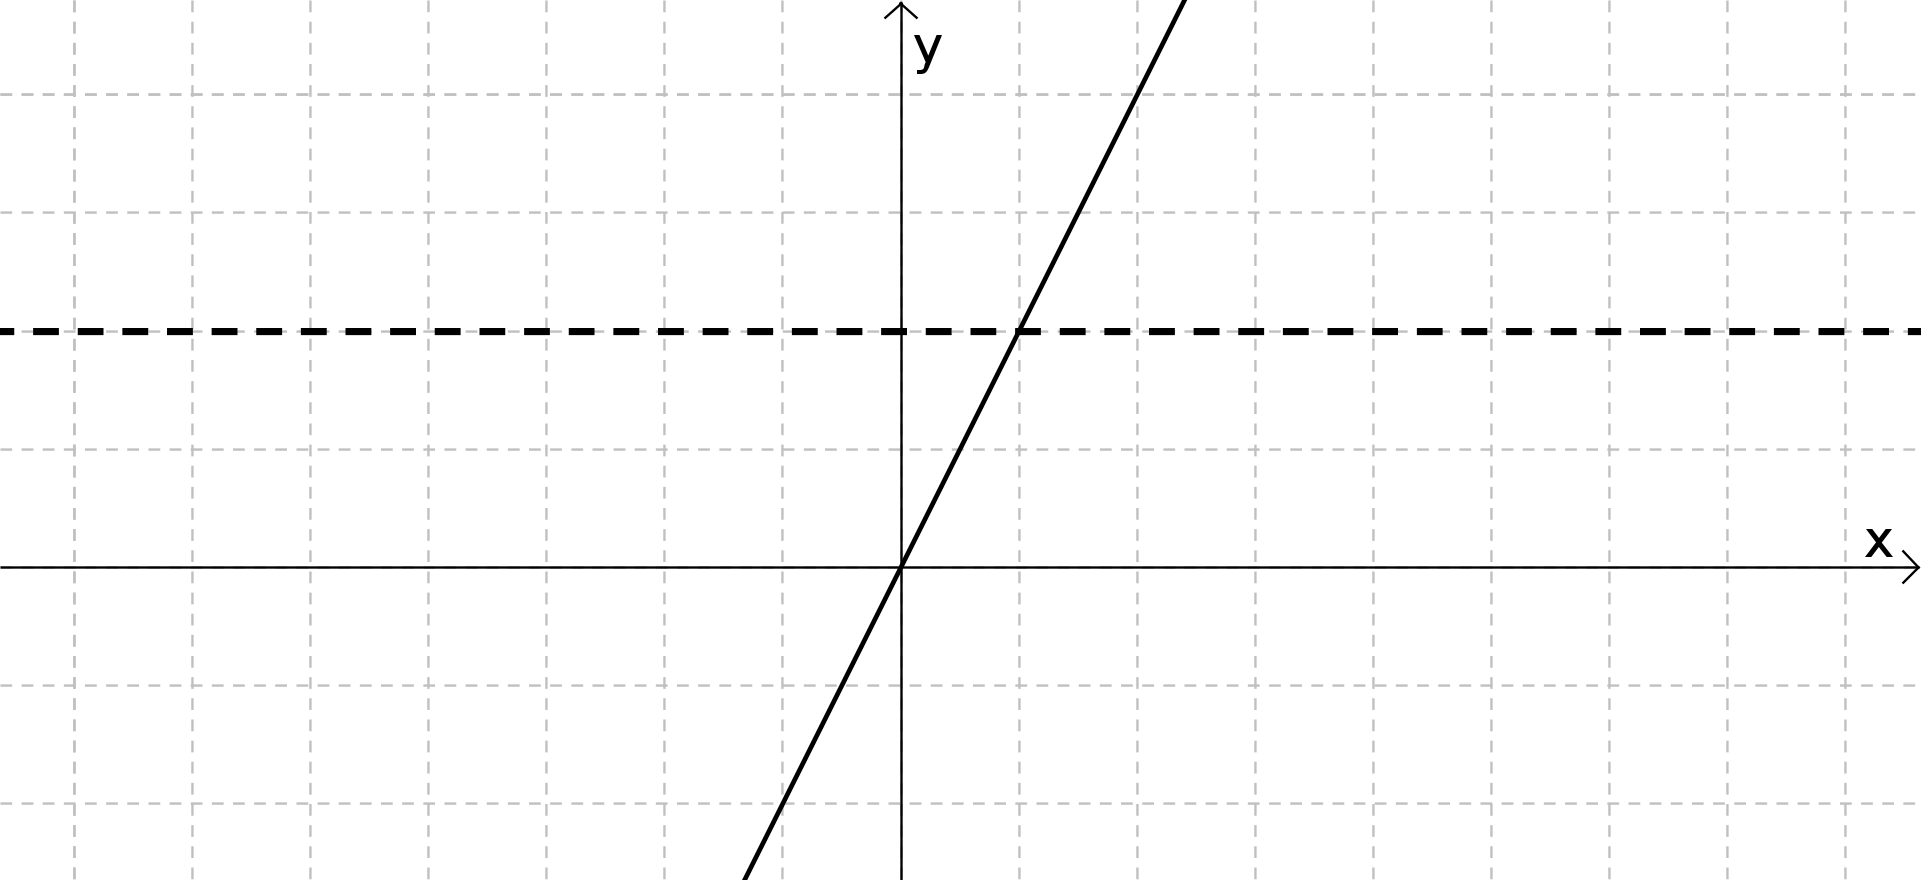
\includegraphics[width=0.5\textwidth]{Philippe/Figures_Philippe/d_riv_es_2_6.png}
                \end{center}
            \end{question}

            \begin{reponses}
                \item[true] La courbe en pointillée est la dérivée de la courbe en trait plein
                \item[false] La courbe en traits pl est la dérivée de la courbe en trait plein
                \item[false] Si la courbe en pointillés est une vitesse en fonction du temps, alors la courbe en traits pleins est une accélération en fonction du temps.
                \item[true] Si la courbe en pointillés est une vitesse en fonction du temps, alors la courbe en traits pleins est une position en fonction du temps.
            \end{reponses}
            %%%%%%%%%%%%%%%%%%%%%%%%%%%%%%%%%%%%%

            \begin{question}{20}{Dérivées}{3}{19}
                La vitesse d'un objet est croissante dans le temps. Quelles affirmations peuvent être vraies à propos de sa position par rapport à un point fixe? (plusieurs réponses possibles)
            \end{question}

            \begin{reponses}
                \item[true] La position est positive.
                \item[true] La position est décroissante.
                \item[true] La position est croissante.
                \item[true] La position est négative.
            \end{reponses}
            %%%%%%%%%%%%%%%%%%%%%%%%%%%%%%%%%%%%%

        \subsection{Savoir calculer une dérivée d'un produit + Dériver les fonctions usuelles}
        
        	\begin{question}{/}{Dérivées}{1}{22 et 23}
				Soient $u$ une fonction définie sur $\mathbb{R}$ par $u(x)=2x$ et $v$ une fonction définie sur $\mathbb{R}$ par  $v(x)=\cos(x)$. Que vaut la dérivée de $u\times v$ par rapport à $x$?
            \end{question}

            \begin{reponses}
            	\item[false] $-2\sin(x)$
            	\item[false] $2-\sin(x)$
                \item[false] $2\cos(x)+2x\sin(x)$
                \item[true] $2\cos(x)-2x\sin(x)$
            \end{reponses}
			%%%%%%%%%%%%%%%%%%%%%%%%%%%%%%%%%%%%%

            \begin{question}{/}{Dérivées}{2}{22 et 23}
                Que vaut la dérivée par rapport à $x$ de la fonction $u$ une fonction définie sur $\mathbb{R}$ par $u(x)=\sin(x)\cos(x)$?
            \end{question}

            \begin{reponses}
                \item[false] $\cos(x)-\sin(x)$
                \item[true] $\cos(x)^2-\sin(x)^2$
                \item[false] $\cos(x)^2+\sin(x)^2$
                \item[false] $\sin(x)^2-\cos(x)^2$
            \end{reponses}
            %%%%%%%%%%%%%%%%%%%%%%%%%%%%%%%%%%%%%

        \subsection{Savoir calculer une dérivée d'un quotient + Savoir calculer une dérivée d'un produit + Dériver les fonctions usuelles}
        
        	\begin{question}{/}{Dérivées}{1}{22 et 23 et 24}
				Soient $v$ et $u$ deux fonctions définies sur $\mathbb{R}$ par $v(x)=2x$ et $u(x)=\cos(x)$. Que vaut la dérivée par rapport à $x$ de $u/v$?
            \end{question}

            \begin{reponses}
            	\item[false] $\frac{2x\sin(x)-2\cos(x)}{4x^2}$
            	\item[false] $\frac{-4x\sin(x)\cos(x)}{4x^2}$
                \item[false] $\frac{4x\sin(x)\cos(x)}{4x^2}$
                \item[true] $\frac{-2x\sin(x)-2\cos(x)}{4x^2}$
            \end{reponses}
			%%%%%%%%%%%%%%%%%%%%%%%%%%%%%%%%%%%%%

            \begin{question}{/}{Dérivées}{2}{22 et 23 et 24}
                Soient $u$ et $v$ deux fonctions définies sur $\mathbb{R}$. Que vaut la dérivée par rapport à $x$ de $u\times v^{-1}$ (deux réponses attendues)?
            \end{question}

            \begin{reponses}
            	\item[false] $(u'v+v'u)v^{-2}$
            	\item[true] $(u'v-v'u)v^{-2}$
                \item[true] $u'v^{-1}-uv'v^{-2}$
                \item[false] $\frac{u'-v'}{v^2}$
            \end{reponses}
            %%%%%%%%%%%%%%%%%%%%%%%%%%%%%%%%%%%%%

            \begin{question}{/}{Dérivées}{2}{22 et 23 et 24}
                Que vaut la dérivée par rapport à $f$ de $\frac{3x^2}{f}$?
            \end{question}

            \begin{reponses}
                \item[false] $\frac{6x}{f}$
                \item[false] $-\frac{6x}{f^2}$
                \item[true] $-\frac{3x^2}{f^2}$
                \item[false] $\ln(3x^2)$
            \end{reponses}
            %%%%%%%%%%%%%%%%%%%%%%%%%%%%%%%%%%%%%

            \begin{question}{/}{Dérivées}{2}{22 et 23 et 24}
                En une dimension, le champ électrique $E$ est égale à $-\frac{dV}{dx}$ avec $V$ le potentiel électrique et $x$ la position. Sachant que $V=k\frac{q}{x}+C$ avec $k$ la constante de Coulomb, $q$ la charge et $C$ une constante quelconque, quelle est l'expression de $E$?
            \end{question}

            \begin{reponses}
                \item[false] $-k\frac{q}{x^2}$
                \item[true] $k\frac{q}{x^2}$
                \item[false] $-kq\ln(x)$
                \item[false] $kq$
            \end{reponses}
            %%%%%%%%%%%%%%%%%%%%%%%%%%%%%%%%%%%%%
        
        	\begin{question}{/}{Dérivées}{3}{22 et 23 et 24}
				Soit $f$ une fonction définie sur $\mathbb{R}$ par  $f(x)=\frac{e^x + e^{-x}}{e^x - e^{-x}}$. Quelle est sa dérivée par rapport à $x$?
            \end{question}

            \begin{reponses}
            	\item[false] $\frac{(e^x + e^{-x})(e^x - e^{-x})}{(e^x - e^{-x})^2}$
            	\item[false] $1-\frac{(e^x - e^{-x})^2}{(e^x + e^{-x})^2}$
                \item[false] $1+\frac{(e^x + e^{-x})^2}{(e^x - e^{-x})^2}$
                \item[true] $1-\frac{(e^x + e^{-x})^2}{(e^x - e^{-x})^2}$
            \end{reponses}
			%%%%%%%%%%%%%%%%%%%%%%%%%%%%%%%%%%%%%

        \subsection{Savoir calculer une dérivée d'une fonction composée + Savoir calculer une dérivée d'un quotient + Savoir calculer une dérivée d'un produit + Dériver les fonctions usuelles}
        
        	\begin{question}{/}{Dérivées}{1}{22 et 23 et 24 et 25}
				Soit $f$ une fonction définie sur $\mathbb{R}$ par $f(x)=e^{3x}$. Quelle est sa dérivée par rapport à $x$?
            \end{question}

            \begin{reponses}
            	\item[true] $3e^{3x}$
            	\item[false] $e^{3x}$
                \item[false] $3e$
                \item[false] $3xe^{3x}$
            \end{reponses}
			%%%%%%%%%%%%%%%%%%%%%%%%%%%%%%%%%%%%%

            \begin{question}{/}{Dérivées}{2}{22 et 23 et 24 et 25}
                Soit $z$ une fonction définie sur $\mathbb{R}$ par de $z(t)=-\sin(\cos(t))$. Que vaut sa dérivée par rapport à $t$?
            \end{question}

            \begin{reponses}
                \item[false] $\cos(t)\sin(\cos(t))-\sin(\cos(t))$
                \item[false] $\cos(t)\sin(\cos(t))$
                \item[true] $\sin(t)\cos(\cos(t))$
                \item[false] $\sin(t)\cos(\cos(t))-\sin(\sin(t))$
            \end{reponses}
            %%%%%%%%%%%%%%%%%%%%%%%%%%%%%%%%%%%%%

            \begin{question}{/}{Dérivées}{2}{22 et 23 et 24 et 25}
                Nous considérons un objet en mouvement circulaire accéléré. L'angle entre le vecteur position et l'axe des $x$ est $\theta(t)=\alpha t^2$ avec $\alpha$ une constante. La composante sur $x$ de la position est donnée par \mbox{$A\cos(\theta(t))=A\cos(\alpha t^2)$}, avec $A$ une constante. Quelle est l'expression de la dérivée de la composante sur $x$ par rapport au temps?
            \end{question}

            \begin{reponses}
                \item[false] $-2\alpha A\sin(\alpha t^2)$
                \item[false] $-A\sin(2\alpha t)$
                \item[false] $-2A\alpha\sin(t)$
                \item[true] $-2\alpha At\sin(\alpha t^2)$
            \end{reponses}
            %%%%%%%%%%%%%%%%%%%%%%%%%%%%%%%%%%%%%

            \begin{question}{/}{Dérivées}{3}{22 et 23 et 24 et 25}
                Soit $f$ une fonction définie sur $\mathbb{R}^2$ par $f(x,y)=\frac{x}{1-y^2}$. Que vaut sa dérivée par rapport à $y$?
            \end{question}

            \begin{reponses}
                \item[true] $\frac{2xy}{(1-y^2)^2}$
                \item[false] $\frac{-2x}{(1-y^2)^2}$
                \item[false] $\frac{2y}{(1-y^2)^2}$
                \item[false] $\frac{-2y}{(1-y^2)^2}$
            \end{reponses}
            %%%%%%%%%%%%%%%%%%%%%%%%%%%%%%%%%%%%%

    \section{Primitives}

        \subsection{Savoir calculer une intégrale connaissant la primitive}
        
        	\begin{question}{60}{Primitives}{1}{/}
				Soit $f$ une fonctions définies sur $\mathbb{R}$ par $f(x)=a$ avec $a$ une constante. Sa primitive par rapport à $x$ est une fonction $g$ définie sur $\mathbb{R}$ par $g(x)=ax$. Que vaux l'intégrale de $1$ à $10$ de la fonction $f$ définie sur $\mathbb{R}$ par $f(x)=3$?
            \end{question}

            \begin{reponses}
            	\item[false] $27x$
            	\item[false] $3x$
                \item[false] 30
                \item[true] 27
            \end{reponses}
			%%%%%%%%%%%%%%%%%%%%%%%%%%%%%%%%%%%%%

            \begin{question}{60}{Primitives}{2}{/}
                Soit $f$ une fonctions définies sur $\mathbb{R}$ par $f(x)=x^n$. Sa primitive par rapport à $x$ est une fonction $g$ définie sur $\mathbb{R}$ par $g(x)=\frac{1}{n+1}x^{n+1}$. Que vaut $\int_{-2}^4 x^2 dx$?
            \end{question}

            \begin{reponses}
                \item[false] 12
                \item[false] 18
                \item[false] 4
                \item[true] 24
            \end{reponses}
            %%%%%%%%%%%%%%%%%%%%%%%%%%%%%%%%%%%%%
        
        	\begin{question}{60}{Primitives}{3}{/}
				Une primitive de $\ln$ est $x\mapsto x\ln(x)-x$. Que vaut $\int_{1}^e \ln(x)dx$?
            \end{question}

            \begin{reponses}
            	\item[false] e
            	\item[false] 0
                \item[true] 1
                \item[false] -1
            \end{reponses}
			%%%%%%%%%%%%%%%%%%%%%%%%%%%%%%%%%%%%%

            \begin{question}{60}{Primitives}{3}{/}
                Le travail d'une force est l'intégrale de la projection du travail sur le chemin parcouru. En termes mathématiques: $W=\int_{x_i}^{x_f}\vec{F}.\vec{dl}$. Un jouet avance de $x_i=0\;\si{\meter}$ à $x_f=2\;\si{\meter}$ le long de l'axe $x$, poussé par une force dirigée selon l'axe $x$ dont l'intensité varie dans l'espace telle que $\vec{F}(x) = (1+\frac{3}{2}x^2)\hat{u}_x$. Le produit scalaire $\vec{F}\cdot\vec{dl}$ devient alors $F\cdot dx$.
                Que vaut le travail de cette force?
            \end{question}

            \begin{reponses}
                \item[true] \SI{6}{J}.
                \item[false] \SI{4}{J}.
                \item[false] \SI{8}{J}.
                \item[false] \SI{2}{J}.
            \end{reponses}
            %%%%%%%%%%%%%%%%%%%%%%%%%%%%%%%%%%%%%

        \subsection{Savoir représenter une intégrale sur un graphe de fonction}
        
        	\begin{question}{1188}{Primitives}{1}{/}
				Que représente l'intégrale d'une fonction par rapport à $x$ entre $A$ et $B$?
            \end{question}

            \begin{reponses}
            	\item[false] La variation de la fonction entre les points $A$ et $B$
                \item[false] La longueur de la courbe de la fonction entre les points $A$ et $B$
            	\item[true] L'aire algébrique (donc possiblement négative) qui est entre la courbe de la fonction et l'axe des $x$, entre les points $A$ et $B$
                \item[false] rien de tout cela
            \end{reponses}
			%%%%%%%%%%%%%%%%%%%%%%%%%%%%%%%%%%%%%

            \begin{question}{1188}{Vecteurs}{2}{/}
                La courbe ci-dessous a pour équation $f(x)=x^2$. Combien vaut la surface délimitée par les points $A$, $B$, $C$ et $D$?
                \begin{center}
                	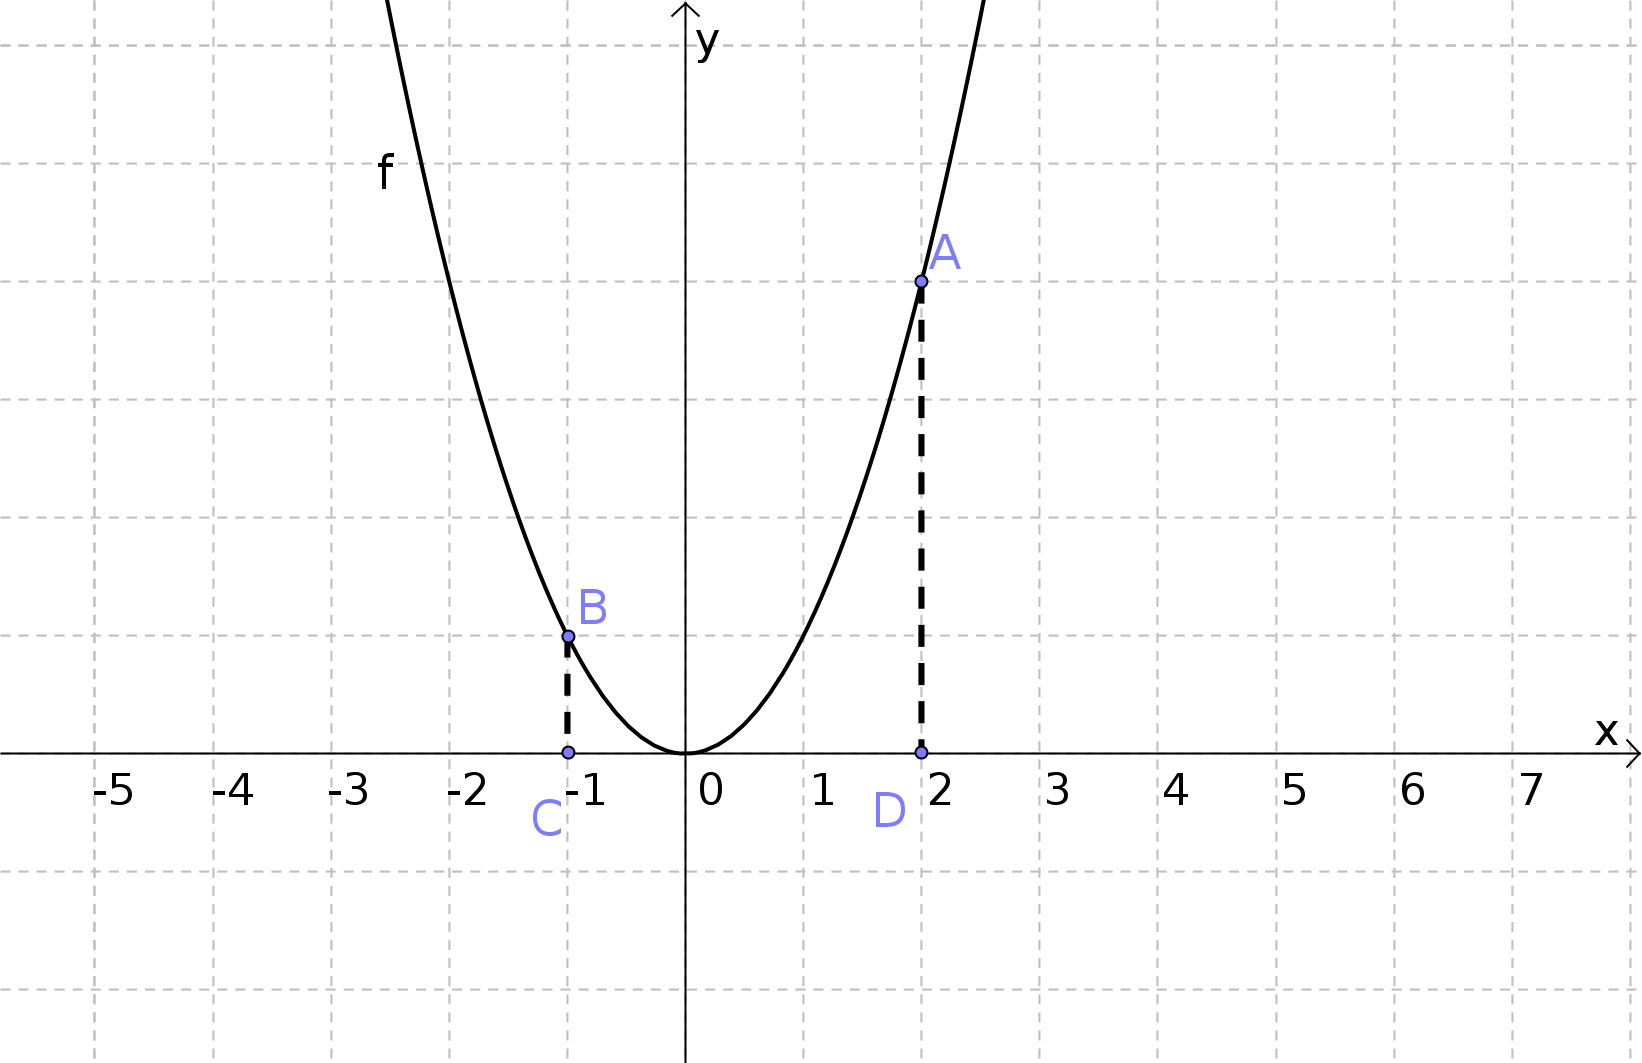
\includegraphics[width=0.5\textwidth]{Philippe/Figures_Philippe/primitives_3_2.png}
                \end{center}
            \end{question}

            \begin{reponses}
                \item[false] 3
                \item[false] $\sqrt{3}$
                \item[false] 4
                \item[true] $\sqrt{4}$ 
            \end{reponses}
            %%%%%%%%%%%%%%%%%%%%%%%%%%%%%%%%%%%%%

            \begin{question}{1188}{Primitives}{2}{/}
                Une fonction $f$ est strictement croissante sur un intervalle. Quelle affirmation est vraie sur le même intervalle?
            \end{question}

            \begin{reponses}
                \item[false] Sa primitive est négative
                \item[true] Sa primitive est positive
                \item[false] Sa primitive est nulle
                \item[false] Aucune de ces affirmations
            \end{reponses}
            %%%%%%%%%%%%%%%%%%%%%%%%%%%%%%%%%%%%%

            \begin{question}{1188}{Primitives}{2}{/}
                Supposons que nous disposions d'un graphique représentant la fonction de la puissance électrique consommée par un foyer en fonction du temps, sur une année entière. Sachant que la puissance est la dérivée de l'énergie par rapport au temps, comment fait-on pour connaître la quantité totale d'énergie consommée dans l'année?
            \end{question}

            \begin{reponses}
                \item[false] On calcule la primitive la fonction.
                \item[false] On calcule la dérivée la fonction.
                \item[true] On calcule l'intégrale la fonction.
                \item[false] On ne peut pas le faire.
            \end{reponses}
            %%%%%%%%%%%%%%%%%%%%%%%%%%%%%%%%%%%%%

        \subsection{Connaître les primitives des fonctions usuelles}
        
        	\begin{question}{61}{Primitives}{1}{22}
				Quelle est la primitive par rapport à $x$ de la fonction $f$ définie sur $\mathbb{R}$ par $f(x)=x$?
            \end{question}

            \begin{reponses}
            	\item[false] $x^2+constante$
            	\item[false] $constante$
                \item[false] $x+constante$
                \item[true] $\frac{1}{2}x^2+constante$
            \end{reponses}
			%%%%%%%%%%%%%%%%%%%%%%%%%%%%%%%%%%%%%
        
        	\begin{question}{61}{Primitives}{1}{22}
				Quelle est la primitive par rapport à $x$ de la fonction $f$ définie sur $\mathbb{R}$ par $f(x)=a.x$ avec $a$ une constante?
            \end{question}

            \begin{reponses}
            	\item[false] $ax+\frac{1}{2}^2+constante$
            	\item[false] $a+constante$
                \item[true] $\frac{a}{2}x^2+constante$
                \item[false] $ax+constante$
            \end{reponses}
			%%%%%%%%%%%%%%%%%%%%%%%%%%%%%%%%%%%%%
        
        	\begin{question}{61}{Primitives}{1}{22}
				Quelle est la primitive par rapport à $x$ de la fonction $f$ définie sur $\mathbb{R}$ par $f(x)=\cos(x)$?
            \end{question}

            \begin{reponses}
            	\item[false] $-\cos(x)+constante$
            	\item[true] $\sin(x)+constante$
                \item[false] $\cos(x)+constante$
                \item[false] $-\sin(x)+constante$
            \end{reponses}
			%%%%%%%%%%%%%%%%%%%%%%%%%%%%%%%%%%%%%
        
        	\begin{question}{61}{Primitives}{1}{22}
				Quelle est la primitive par rapport à $x$ de la fonction $f$ définie sur $\mathbb{R}$ par $f(x)=\sin(x)$?
            \end{question}

            \begin{reponses}
            	\item[true] $-\cos(x)+constante$
            	\item[false] $\sin(x)+constante$
                \item[false] $\cos(x)+constante$
                \item[false] $-\sin(x)+constante$
            \end{reponses}
			%%%%%%%%%%%%%%%%%%%%%%%%%%%%%%%%%%%%%
        
        	\begin{question}{61}{Primitives}{2}{22}
				Quelle est la primitive par rapport à $x$ de la fonction $f$ définie sur $\mathbb{R}$ par $f(x)=\cos(a.x)$?
            \end{question}

            \begin{reponses}
            	\item[false] $a.\sin(x)+constante$
            	\item[true] $\frac{1}{a}\sin(a.x)+constante$
                \item[false] $a.\sin(a.x)+constante$
                \item[false] $\frac{1}{a}\sin(x)+constante$
            \end{reponses}
			%%%%%%%%%%%%%%%%%%%%%%%%%%%%%%%%%%%%%
        
        	\begin{question}{61}{Primitives}{2}{22}
				Quelle est la primitive par rapport à $x$ de la fonction $f$ définie sur $\mathbb{R^*}$ par $f(x)=\frac{1}{x}$?
            \end{question}

            \begin{reponses}
            	\item[false] $1+constante$
            	\item[true] $ln(|x|)+constante$
                \item[false] Pas de solution (on ne peut pas diviser par $0$)
                \item[false] $e^x$
            \end{reponses}
			%%%%%%%%%%%%%%%%%%%%%%%%%%%%%%%%%%%%%

            \begin{question}{61}{Primitives}{2}{22}
                Laquelle de ces fonctions est une primitive de $x\mapsto \frac{2}{x^2}$? 
            \end{question}

            \begin{reponses}
                \item[true] $-\frac{2}{x}$
                \item[false] $\frac{-4}{x^3}$
                \item[false] $\frac{2}{x}$
                \item[false] $\frac{4}{x^3}$
            \end{reponses}
            %%%%%%%%%%%%%%%%%%%%%%%%%%%%%%%%%%%%%

            \begin{question}{61}{Primitives}{2}{22}
                La vitesse angulaire d'un pendule oscillant est donnée, dans l'approximation des petits angles et en négligeant les frottements, par $\dot{\theta}=-\theta_0\cdot\omega\cdot\sin(\omega t)$, avec $\theta_0$ et $\omega$ des constantes. Quelle est l'expression de $\theta(t)$?
            \end{question}

			\begin{reponses}
                \item[false] $-\theta_0\cdot\cos(\omega t)+constante$
                \item[false] $-\theta_0\cdot\cos(\omega t)$
                \item[false] $-\theta_0\cdot\cos(\omega t)$
                \item[true] $\theta_0\cdot\cos(\omega t)+constante$
            \end{reponses}
            %%%%%%%%%%%%%%%%%%%%%%%%%%%%%%%%%%%%%
        
        	\begin{question}{61}{Primitives}{3}{22}
				Quelle est la primitive par rapport à $x$ de $f(x)=x^n$?
            \end{question}

            \begin{reponses}
            	\item[true] $\frac{1}{n+1}x^{n+1}$
            	\item[false] $\frac{1}{n-1}x^{n-1}$
                \item[false] ${n}x^{n+1}$
                \item[false] $\frac{1}{n}x^{n-1}$
            \end{reponses}
			%%%%%%%%%%%%%%%%%%%%%%%%%%%%%%%%%%%%%

    \section{Vecteurs}

        \subsection{Savoir ce qu'est un vecteur}
        
        	\begin{question}{non créé}{Vecteurs}{1}{/}
				Soit $\vec{A}$ un vecteur en deux dimensions. Sa coordonnée sur l'axe $x$ est $a_x$, et sa coordonnée sur l'axe $y$ est $a_y$. Laquelle de ces quantité est égale à $\vec{A}$?
            \end{question}

            \begin{reponses}
            	\item[false] $(a_x+a_y;a_x-a_y)$
            	\item[true] $a_x\vec{u_x}+a_y\vec{u_y}$ où $\vec{u_x}$ et $\vec{u_y}$ sont les vecteurs unitaires des axes $x$ et $y$
                \item[false] $\sqrt{a_{x}^2+a_{y}^2}$
                \item[false] $(\sqrt{a_{x}^2+a_{y}^2};\sqrt{a_{x}^2-a_{y}^2})$
            \end{reponses}
			%%%%%%%%%%%%%%%%%%%%%%%%%%%%%%%%%%%%%

        \subsection{Calculer la norme d'un vecteur}
        
        	\begin{question}{1202}{Vecteurs}{1}{/}
				Soit un vecteur $\vec{A}=(a_x;a_y)$. Quelle est la norme de ce vecteur?
            \end{question}

            \begin{reponses}
            	\item[false] $a_x+a_y$
            	\item[false] $a_x\times a_y$
                \item[false] $a_{x}^2+a_{y}^2$
                \item[true] $\sqrt{a_{x}^2+a_{y}^2}$
            \end{reponses}
			%%%%%%%%%%%%%%%%%%%%%%%%%%%%%%%%%%%%%
        
        	\begin{question}{1202}{Vecteurs}{1}{/}
				Soit un vecteur $\vec{A}=(a_x;a_y;a_z)$. Quelle est la norme de ce vecteur?
            \end{question}

            \begin{reponses}
            	\item[false] $a_x+a_y+a_z$
            	\item[false] $a_x\times a_y\times a_z$
                \item[false] $a_{x}^2+a_{y}^2+a_{z}^2$
                \item[true] $\sqrt{a_{x}^2+a_{y}^2+a_{z}^2}$
            \end{reponses}
			%%%%%%%%%%%%%%%%%%%%%%%%%%%%%%%%%%%%%

            \begin{question}{1202}{Vecteurs}{2}{/}
                Quelle est la norme du vecteur $\vec{AB}$?
                \begin{center}
                	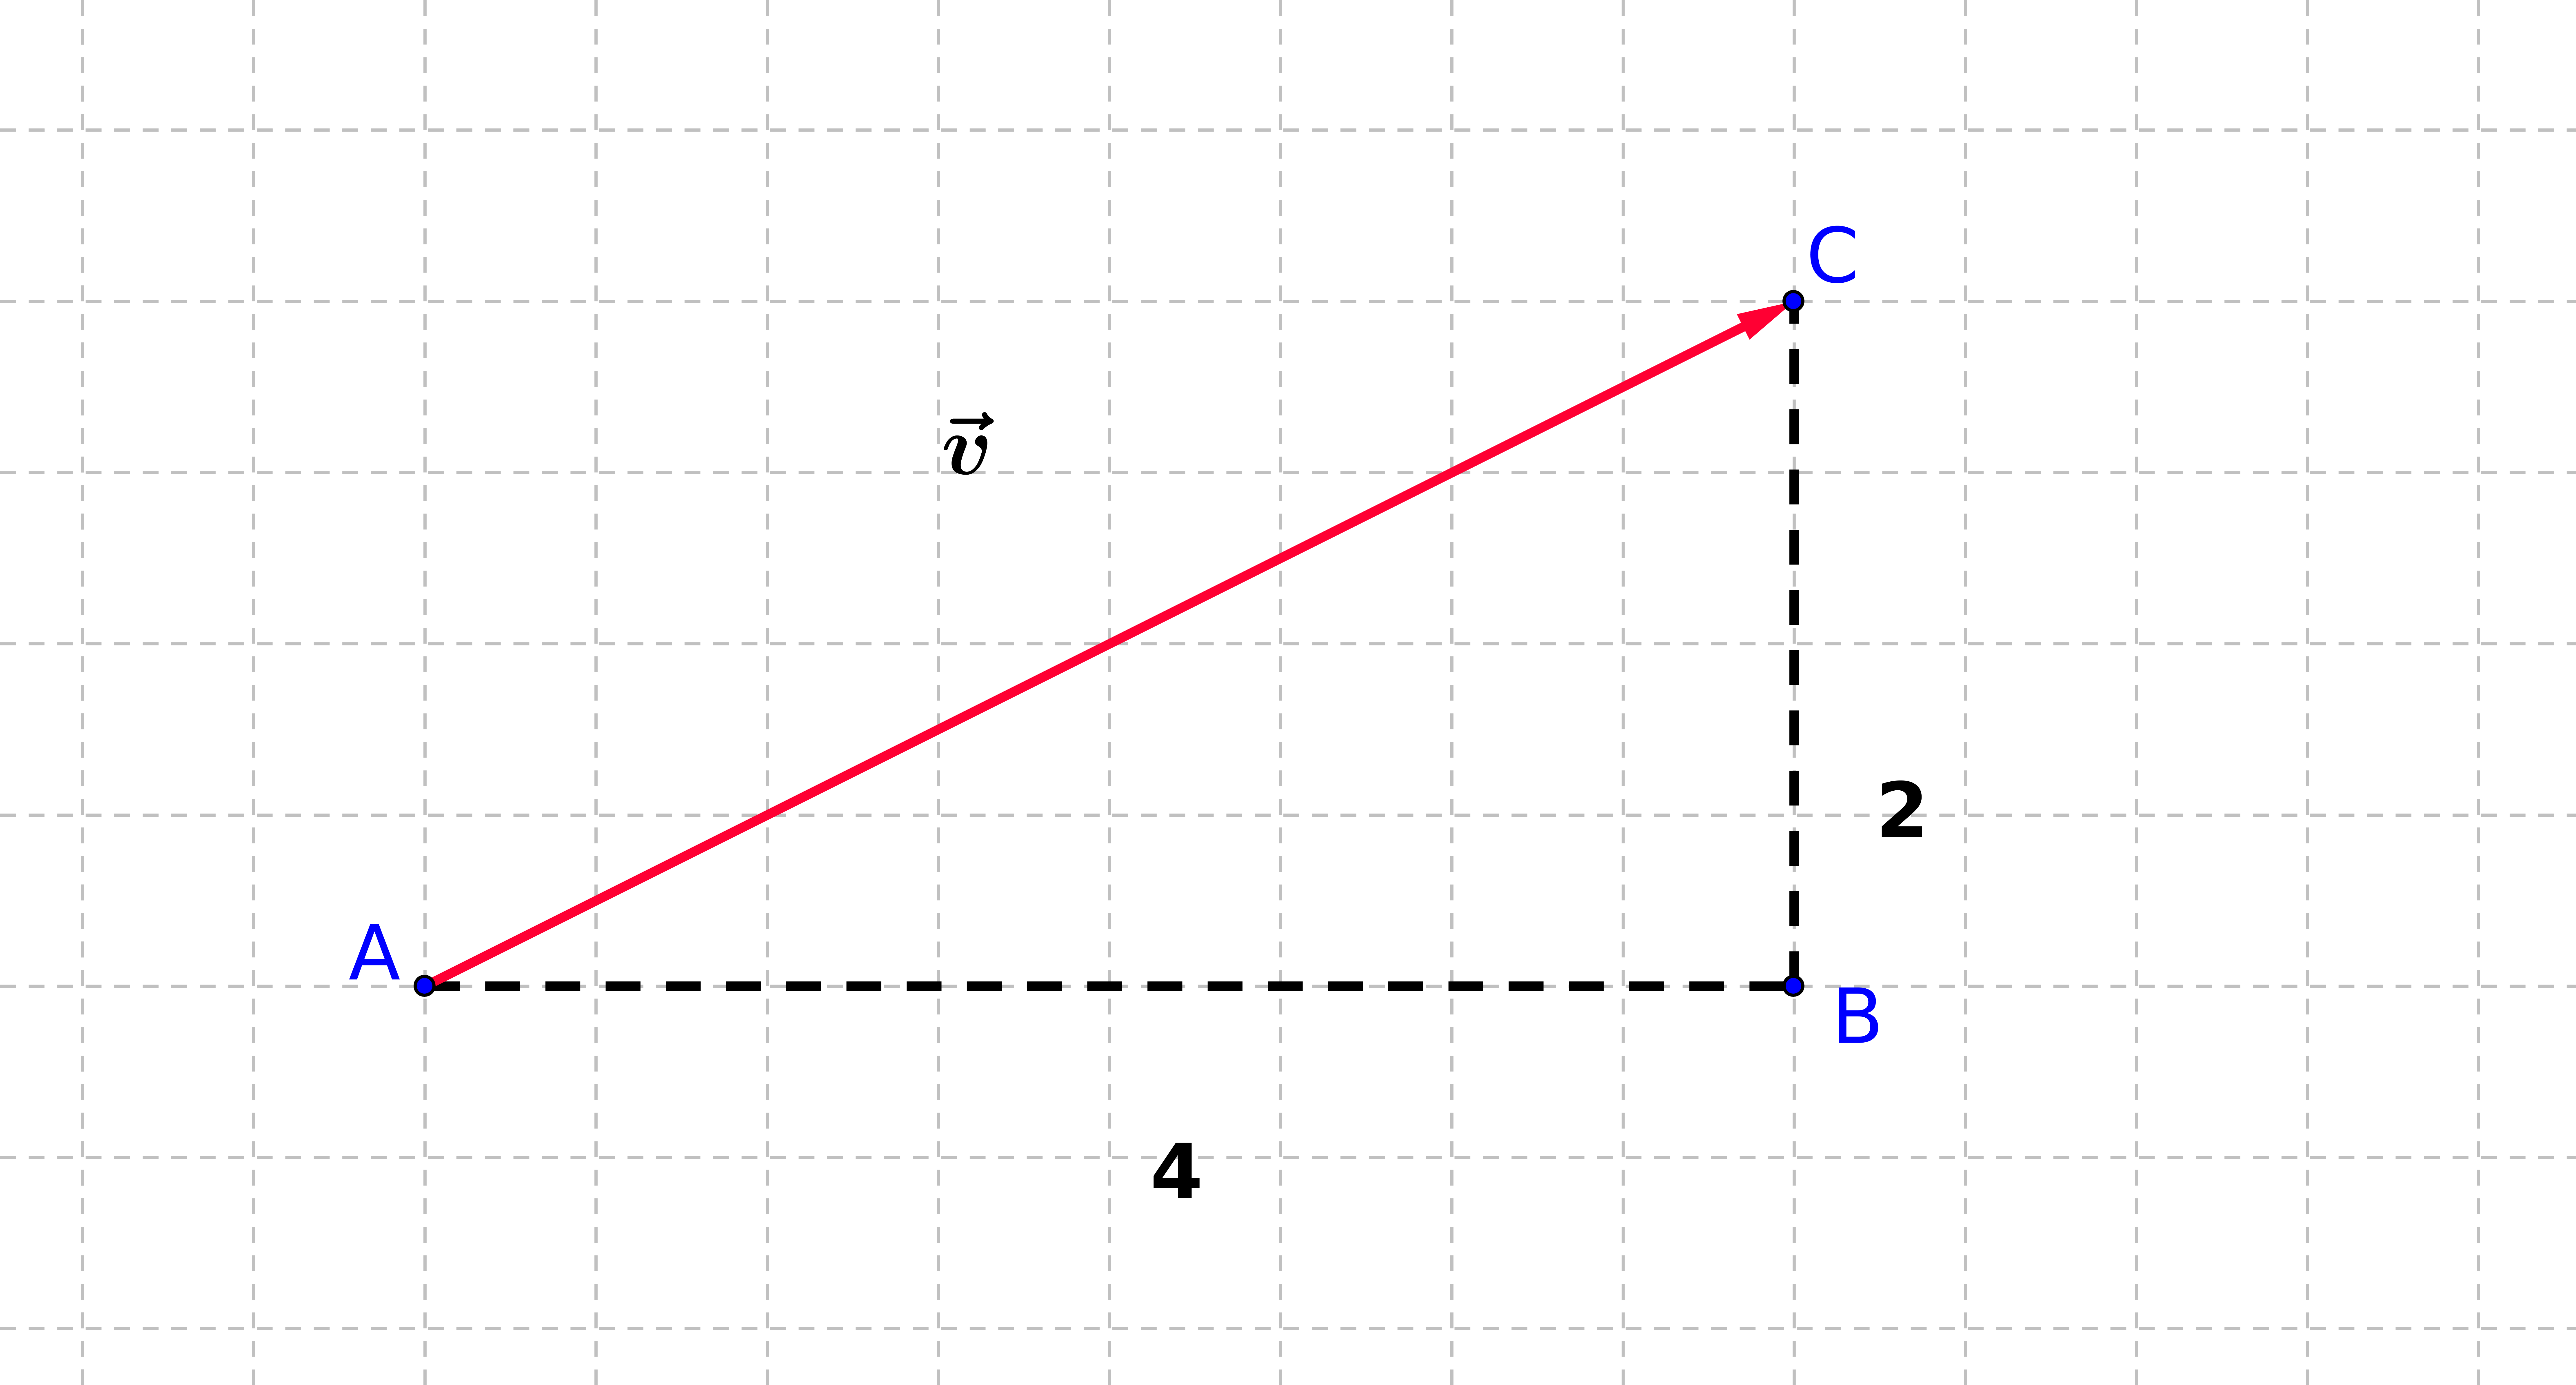
\includegraphics[width=0.5\textwidth]{Philippe/Figures_Philippe/vecteurs_4_2.png}
                \end{center}
            \end{question}

            \begin{reponses}
                \item[false] 6
                \item[false] $\sqrt{6}$
                \item[false] $20$
                \item[true] $\sqrt{20}$ 
            \end{reponses}
            %%%%%%%%%%%%%%%%%%%%%%%%%%%%%%%%%%%%%

            \begin{question}{1202}{Vecteurs}{2}{/}
                Un vecteur a pour coordonnées dans le plan: $x = 4$ et $y = 3$. Combien vaut sa norme?
            \end{question}

            \begin{reponses}
                \item[false] 6
                \item[true] 5
                \item[false] 7
                \item[false] 12
            \end{reponses}
            %%%%%%%%%%%%%%%%%%%%%%%%%%%%%%%%%%%%%

            \begin{question}{1202}{Vecteurs}{2}{/}
                Quelle est la norme $F$ du vecteur force de coordonnées dans le plan $\vec{F}=(12;5)$?
            \end{question}

            \begin{reponses}
                \item[true] \SI{13}{\newton}.
                \item[false] \SI{14}{\newton}.
                \item[false] \SI{15}{\newton}.
                \item[false] \SI{18}{\newton}.
            \end{reponses}
            %%%%%%%%%%%%%%%%%%%%%%%%%%%%%%%%%%%%%

        \subsection{Déterminer les composantes d'un vecteur dans un repère orthonormé à partir des coordonnées des points de départ et d'arrivée}
        
        	\begin{question}{1201}{Vecteurs}{1}{1220}
				Dans un repère à deux dimensions, quelles sont les coordonnées du vecteur allant du point $(0;0)$ au point $(1;2)$?
            \end{question}

            \begin{reponses}
            	\item[false] $(-1;-2)$
            	\item[false] $(2;1)$
                \item[false] $(-2;-1)$
                \item[true] $(1;2)$
            \end{reponses}
			%%%%%%%%%%%%%%%%%%%%%%%%%%%%%%%%%%%%%

            \begin{question}{1201}{Vecteurs}{2}{1220}
                Quelles sont les coordonnées du vecteur $\vec{AB}$?
                \begin{center}
                	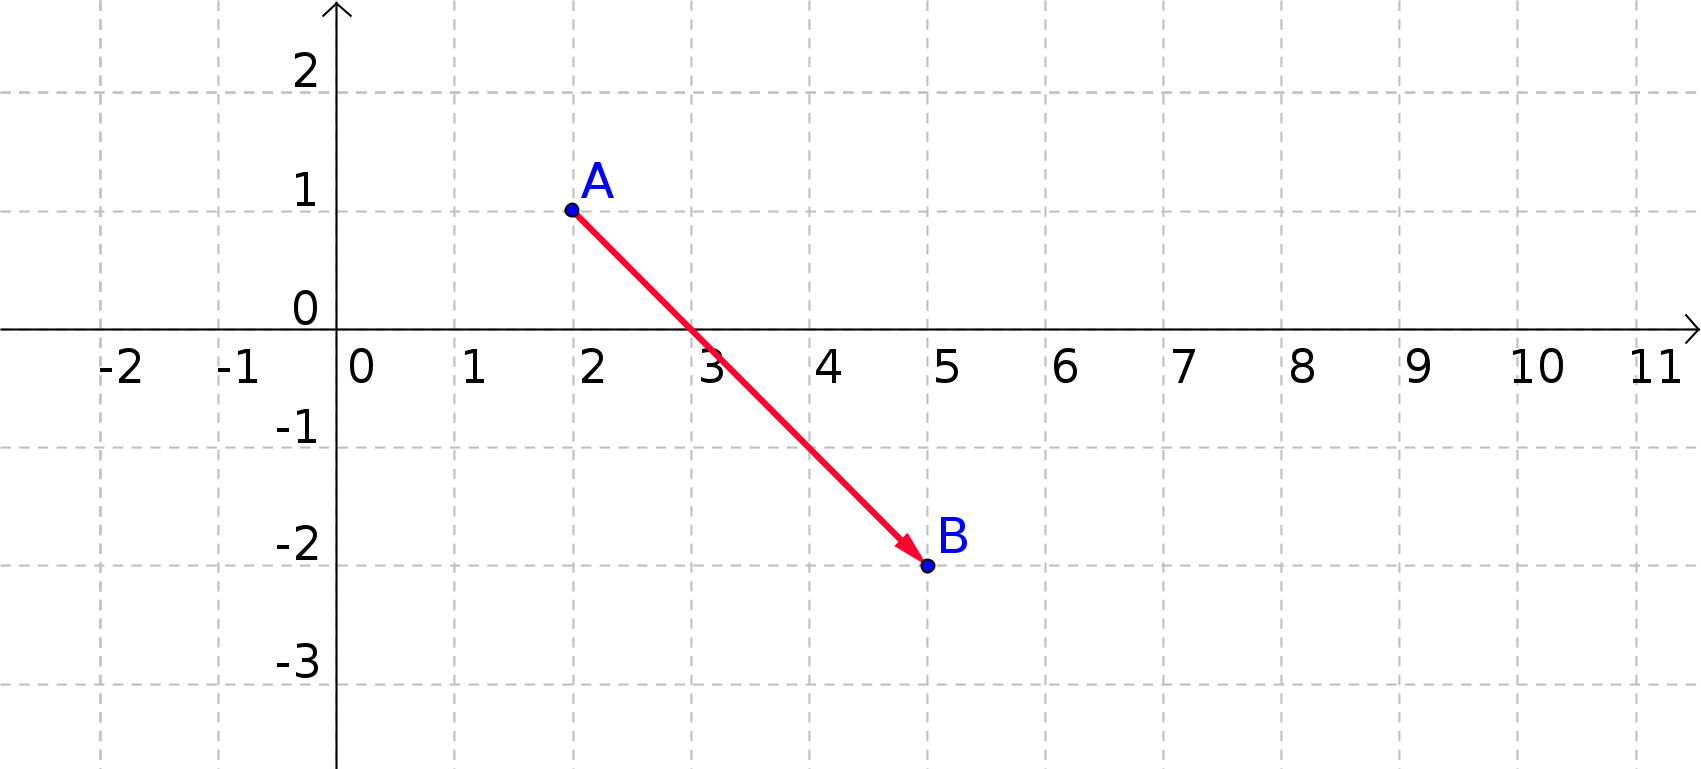
\includegraphics[width=0.5\textwidth]{Philippe/Figures_Philippe/vecteurs_4_3.png}
                \end{center}
            \end{question}

            \begin{reponses}
                \item[false] $(5;-2)$
                \item[false] $(3;3)$
                \item[false] $(-3;3)$
                \item[true] $(3;-3)$ 
            \end{reponses}
            %%%%%%%%%%%%%%%%%%%%%%%%%%%%%%%%%%%%%

            \begin{question}{1201}{Vecteurs}{2}{1220}
                Dans l'espace à trois dimensions, quelles sont les coordonnées du vecteur allant du point $(12;-2;6)$ au point $(-1;0;3)$?
            \end{question}

            \begin{reponses}
                \item[true] $(-13;2;-3)$
                \item[false] $(13;-2;3)$
                \item[false] $(11;2;9)$
                \item[false] $(11;2;3)$
            \end{reponses}
            %%%%%%%%%%%%%%%%%%%%%%%%%%%%%%%%%%%%%

            \begin{question}{1201}{Vecteurs}{2}{1220}
                On donne la position du centre de la Terre comme étant en $(200;542;865)$ et la position d'un satellite en $(-412;-102;623)$. Quelles sont les coordonnées du vecteur reliant le centre de la Terre au satellite?
            \end{question}

            \begin{reponses}
                \item[false] $(612;644;242)$
                \item[false] $(-212;440;242)$
                \item[false] $(212;-440;-242)$
                \item[true] $(-612;-644;-242)$
            \end{reponses}
            %%%%%%%%%%%%%%%%%%%%%%%%%%%%%%%%%%%%%
            
            \begin{question}{/}{Vecteurs}{2}{1217,31,1213}
                Que valent les coordonnées $x$ et $y$ du vecteur $\vec{OM}$ ci-dessous? \\ 
            \begin{tikzpicture}[scale=3, axis/.style={->,blue,thick}, vector/.style={-stealth,red,very thick}, vector guide/.style={dashed,red,thick}]
                \coordinate[label=below  left:O] (O) at (0cm,0cm);
                \coordinate[label=below  left:] (x) at (1cm,0cm);
                \draw[axis] (0,0) -- (1,0) node[anchor=north east]{$x$};
                \draw[axis] (0,0) -- (0,1) node[anchor=north west]{$y$};
                \draw[-Stealth] (O) to ["$OM=3$",sloped] ++ (150.0:3) coordinate[label=above right:M] (M);
                \draw[densely dotted] (O) to ["$x$"] ++ (0:-2.59) coordinate (Mx);
                \draw[densely dotted] (Mx) to ["$y$"] ++ (90:1.5);
                \pic ["$\theta=5\pi/6$", draw=red,->, angle radius = 12mm, angle eccentricity=1.3] {angle = x--O--M};
            \end{tikzpicture}
            \end{question}
            
            \begin{reponses}
                \item[false] $x$ = $3\sqrt{3}$ et $y$ = $-3$
                \item[false] $x$ = $-3$ et $y$ = $0$
                \item[false] $x$ = $3\sqrt{2}/2$ et $y$ = $-3\sqrt{2}/2$
                \item[true] $x$ = $-3\sqrt{3}/2$ et $y$ = $3/2$
            \end{reponses}

        \subsection{Calculer la somme ou la différence de vecteurs en utilisant leurs composantes}
        
        	\begin{question}{1204}{Vecteurs}{1}{1220}
            	Soient deux vecteurs dans l'espace à 2 dimensions $\vec{A}=(1;1)$ et $\vec{B}=(3;3)$. Quelles sont les coordonnées de $\vec{A}+\vec{B}$?
            \end{question}

            \begin{reponses}
            	\item[false] $(-2;-2)$
            	\item[false] $(2;2)$
                \item[true] $(4;4)$
                \item[false] $(0;0)$
            \end{reponses}
			%%%%%%%%%%%%%%%%%%%%%%%%%%%%%%%%%%%%%

            \begin{question}{1204}{Vecteurs}{2}{1220}
                Quelles sont les coordonnées du vecteur $\vec{AB}+\vec{CD}$?
                \begin{center}
                	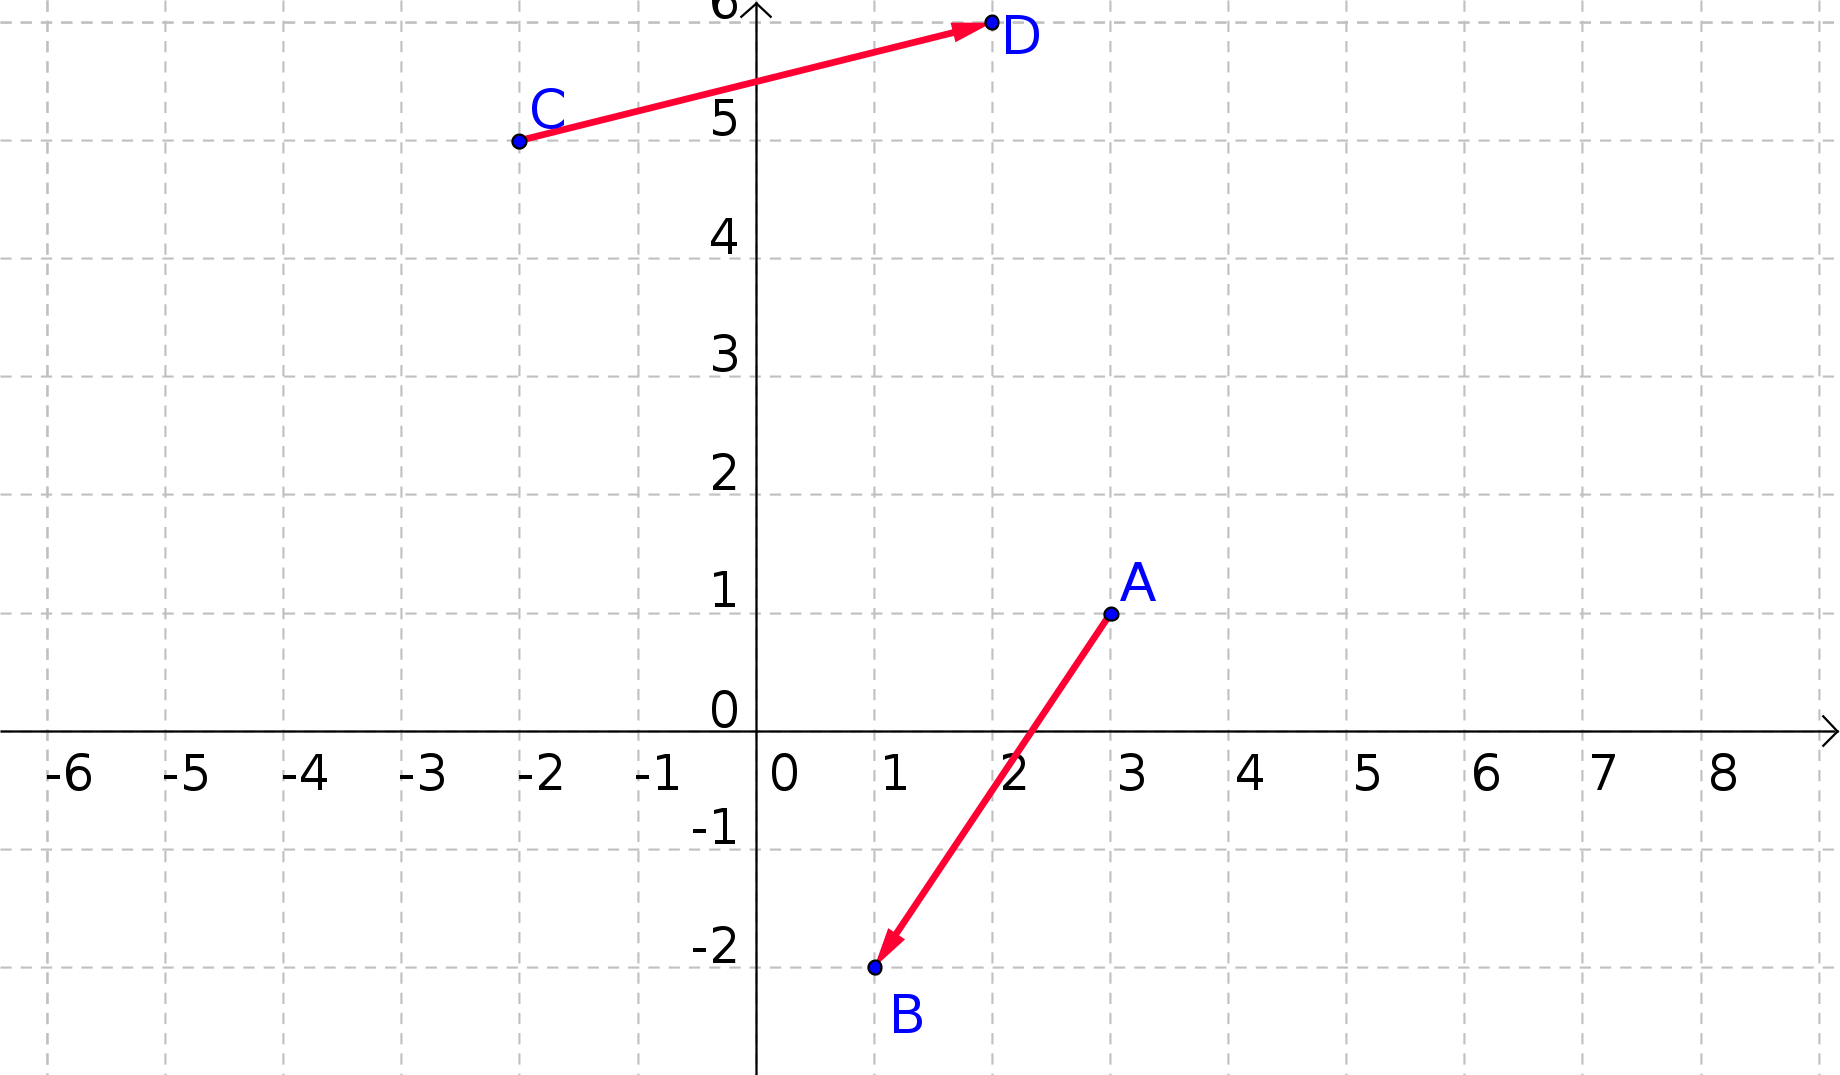
\includegraphics[width=0.5\textwidth]{Philippe/Figures_Philippe/vecteurs_4_4.png}
                \end{center}
            \end{question}

            \begin{reponses}
                \item[false] $(5;7)$
                \item[true] $(2;-2)$
                \item[false] $(-1;-7)$
                \item[false] $(6;4)$
            \end{reponses}
            %%%%%%%%%%%%%%%%%%%%%%%%%%%%%%%%%%%%%

            \begin{question}{1204}{Vecteurs}{2}{1220}
               Soient deux vecteurs de l'espace à 3 dimensions $\vec{A}=(4;2;-2)$ et $\vec{B}=(2;6;1)$. Quelles sont les coordonnées de $\vec{B}-\vec{A}$?
            \end{question}

            \begin{reponses}
                \item[false] $(2;-4;-3)$
                \item[false] $(8;12;2)$
                \item[false] $(-8;-12;-2)$
                \item[true] $(-2;4;3)$
            \end{reponses}
            %%%%%%%%%%%%%%%%%%%%%%%%%%%%%%%%%%%%%

            \begin{question}{1204}{Vecteurs}{2}{1220}
                On sait que la somme des forces extérieures s'appliquant à un objet est égale à la masse multipliée par l'accélération de cet objet. Une masse de \SI{1}{\kilo\gram} subit une force $\vec{F_1}=(0;1;2)$ et une force $\vec{F_2}=(-2;4;-5)$ (en Newton). Que vaut son accélération en \si{\meter\per\second\squared}?
            \end{question}

            \begin{reponses}
                \item[false] $(2;-3;7)$
                \item[false] $(2;-3;3)$
                \item[false] $(-1;-2;5)$
                \item[true] $(-2;5;-3)$
            \end{reponses}
            %%%%%%%%%%%%%%%%%%%%%%%%%%%%%%%%%%%%%

        \subsection{Calculer le produit scalaire entre deux vecteurs}
        
            \begin{question}{1205}{Vecteurs}{1}{1220}
				Quelle est la nature du résultat du produit scalaire de deux vecteurs ?
            \end{question}

            \begin{reponses}
            	\item[false] Un vecteur
            	\item[true] Un nombre
                \item[false] Une fonction
            \end{reponses}
			%%%%%%%%%%%%%%%%%%%%%%%%%%%%%%%%%%%%%
            
        	\begin{question}{1205}{Vecteurs}{1}{1220}
				Soit $\vec{A}=(a_x;a_y)$ et $\vec{B}=(b_x;b_y)$, quel est le produit scalaire entre $\vec{A}$ et $\vec{B}$?
            \end{question}

            \begin{reponses}
            	\item[false] $(a_x+b_x;a_y+b_y)$
            	\item[false] $a_x\times b_x\times \cos(\widehat{a_y b_y})$
                \item[false] $(a_x+b_x)\times (a_y+b_y)$
                \item[true] $a_x\times b_x+a_y\times b_y$
            \end{reponses}
			%%%%%%%%%%%%%%%%%%%%%%%%%%%%%%%%%%%%%
        
        	\begin{question}{1205}{Vecteurs}{1}{1220}
				Soient deux vecteur $\vec{A}$ et $\vec{B}$. On connaît leurs normes ($||\vec{A}||$ et $||\vec{B}||$) et l'angle entre les deux ($\widehat{AB}$). Quel est le produit scalaire entre $\vec{A}$ et $\vec{B}$?
            \end{question}

            \begin{reponses}
            	\item[true] $||\vec{A}||\times ||\vec{B}||\times \cos(\widehat{AB})$
            	\item[false] $||\vec{A}||\times ||\vec{B}||\times \sin(\widehat{AB})$
                \item[false] $||\vec{A}||+||\vec{B}||$
                \item[false] $||\vec{A}||\times ||\vec{B}||$
            \end{reponses}
			%%%%%%%%%%%%%%%%%%%%%%%%%%%%%%%%%%%%%

            \begin{question}{1205}{Vecteurs}{2}{1201}
                Combien vaut le produit scalaire entre $\vec{AB}$ et $\vec{CD}$?\\
                \begin{center}
                	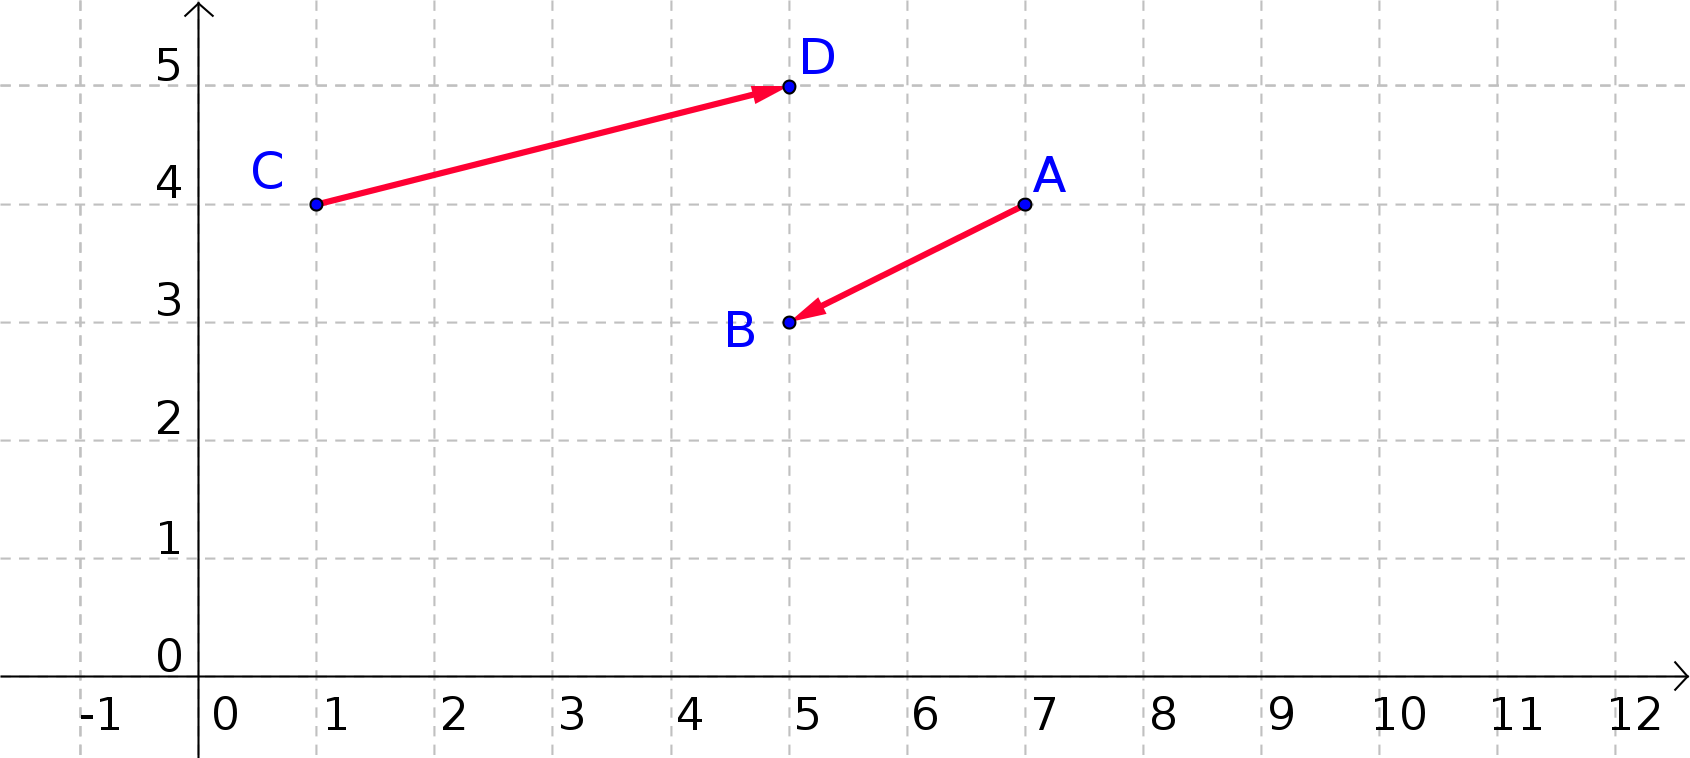
\includegraphics[width=0.5\textwidth]{Philippe/Figures_Philippe/vecteurs_4_5.png}
                \end{center}
            \end{question}

            \begin{reponses}
                \item[true] -9
                \item[false] -21
                \item[false] -55
                \item[false] -7 
            \end{reponses}
            %%%%%%%%%%%%%%%%%%%%%%%%%%%%%%%%%%%%%

            \begin{question}{1205}{Vecteurs}{2}{1220}
                Calculez le produit scalaire des vecteurs $\vec{A}=(4;2;1)$ et $\vec{B}=(1;0;6)$.
            \end{question}

            \begin{reponses}
                \item[true] 10
                \item[false] 11
                \item[false] 42
                \item[false] 14
            \end{reponses}
            %%%%%%%%%%%%%%%%%%%%%%%%%%%%%%%%%%%%%
            
            \begin{question}{1205}{Vecteurs}{2}{1217,31,1213}
                Que vaut le produit scalaire entre les deux vecteurs ci-dessous?
                \begin{figure}
                    \centering
                    \begin{tikzpicture}[scale=3, axis/.style={->,blue,thick}, vector/.style={-stealth,red,very thick}, vector guide/.style={dashed,red,thick}]
                        \coordinate[label=below  left:O] (O) at     (0cm,0cm);
                        \coordinate[label=below  left:] (x) at     (1cm,0cm);
                        \draw[axis] (0,0) -- (1,0) node[anchor=north         east]{$x$};
                        \draw[axis] (0,0) -- (0,1) node[anchor=north         west]{$y$};
                        \draw[-Stealth] (O) to [] ++ (480.0:2)         coordinate[label=above right:M] (M);
                        \draw[densely dotted] (O) to ["$x=-1$"] ++     (0:-1.0)     coordinate (Mx);
                        \draw[densely dotted] (Mx) to ["$y=\sqrt{3}$"]     ++     (90:1.73);
                        \pic["$\theta$", draw=red,->, angle radius =     12mm, angle eccentricity=1.3] {angle = x--O--M};
                    \end{tikzpicture} 
                    \begin{tikzpicture}[scale=3, axis/.style={->,blue,thick}, vector/.style={-stealth,red,very thick}, vector guide/.style={dashed,red,thick}]
                        \coordinate[label=below  left:O] (O) at     (0cm,0cm);
                        \coordinate[label=below  left:] (x) at     (1cm,0cm);
                        \draw[axis] (0,0) -- (1,0) node[anchor=north         east]{$x$};
                        \draw[axis] (0,0) -- (0,1) node[anchor=north         west]{$y$};
                        \draw[-Stealth] (O) to [] ++ (0:3)         coordinate[label=above right:M'] (M');
                        \draw[densely dotted] (O) to [] ++ (0:3.0)         coordinate (Mx);
                        \draw[densely dotted] (Mx) to [] ++ (90:0.0);
                        \draw (1,1) node[right]{$x'=3$, $y'=0$ };
                    \end{tikzpicture}
                \end{figure}
            \end{question}
            \begin{reponses}
                \item[true] \num{-3.0}
                \item[false] \num{-9.0}
                \item[false] \num{-10.92}
                \item[false] \num{-10.93}
            \end{reponses}

            \begin{question}{1205}{Vecteurs}{2}{1220}
                Le couplage d'un système ayant un moment magnétique $\vec{\mu}$ avec un champ magnétique $\vec{B}$ modifie l'énergie du système d'une quantité $\Delta E=-\vec{\mu}\cdot\vec{B}$. Que vaut cette quantité quand $\vec{\mu}=(2;-6;5)$ et $\vec{B}=(-3;1;-6)$?
            \end{question}

            \begin{reponses}
                \item[false] $E=7$
                \item[false] $E=-42$
                \item[false] $E=-7$
                \item[true] $E=42$
            \end{reponses}
            %%%%%%%%%%%%%%%%%%%%%%%%%%%%%%%%%%%%%

        \subsection{Déterminer les composantes d'un vecteur dans un repère orthonormé à partir de la norme et de l'angle}
        
        	\begin{question}{1206}{Vecteurs}{1}{1217}
				Soit $\vec{A}=(a_x;a_y)$ un vecteur. Quel est le lien entre sa norme, sa composante sur $x$ et l'angle $\theta$ entre $\vec{A}$ et l'axe $x$?
            \end{question}

            \begin{reponses}
            	\item[true] $\cos(\theta)=\frac{a_x}{||\vec{A}||}$
            	\item[false] $\sin(\theta)=\frac{a_x}{||\vec{A}||}$
                \item[false] $\cos(\theta)=\frac{||\vec{A}||}{a_x}$
                \item[false] $\sin(\theta)=\frac{||\vec{A}||}{a_x}$
            \end{reponses}
			%%%%%%%%%%%%%%%%%%%%%%%%%%%%%%%%%%%%%
        
        	\begin{question}{1206}{Vecteurs}{1}{1217}
				Soit $\vec{A}=(a_x;a_y)$ un vecteur. Quel est le lien entre sa norme, sa composante sur $y$ et l'angle $\theta$ entre $\vec{A}$ et l'axe $x$?
            \end{question}

            \begin{reponses}
            	\item[false] $\cos(\theta)=\frac{a_y}{||\vec{A}||}$
            	\item[true] $\sin(\theta)=\frac{a_y}{||\vec{A}||}$
                \item[false] $\cos(\theta)=\frac{||\vec{A}||}{a_y}$
                \item[false] $\sin(\theta)=\frac{||\vec{A}||}{a_y}$
            \end{reponses}
			%%%%%%%%%%%%%%%%%%%%%%%%%%%%%%%%%%%%%

            \begin{question}{1206}{Vecteurs}{2}{1217}
                Quelles sont les composantes du vecteur $\vec{AB}$?\\
                \begin{center}
                	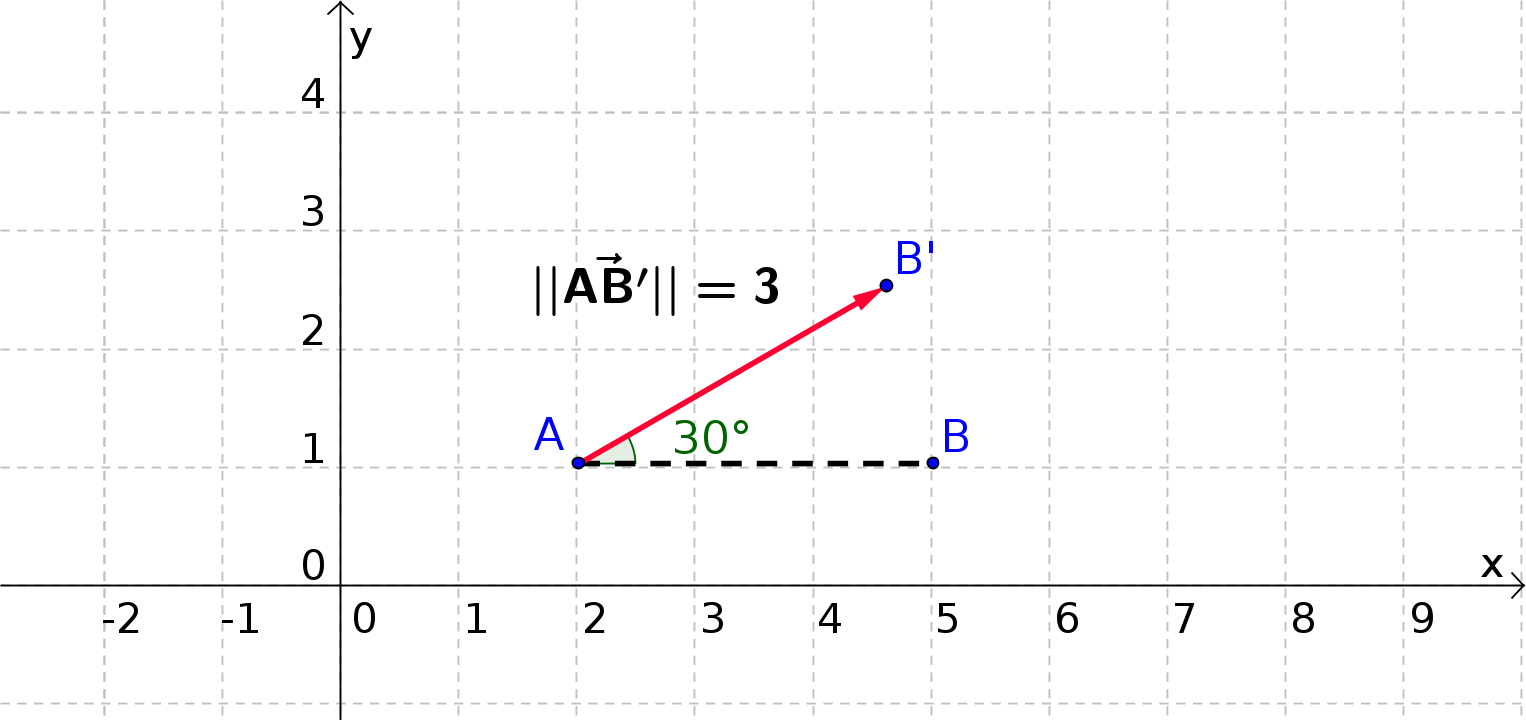
\includegraphics[width=0.5\textwidth]{Philippe/Figures_Philippe/vecteurs_4_6.png}
                \end{center}
            \end{question}

            \begin{reponses}
                \item[false] $(5;2.5)$
                \item[false] $(3;1)$
                \item[false] $(3;1,5)$
                \item[true] $(3\sqrt{3}/2;1,5)$
            \end{reponses}
            %%%%%%%%%%%%%%%%%%%%%%%%%%%%%%%%%%%%%
        
        	\begin{question}{1206}{Vecteurs}{2}{1217}
				Soit $\vec{A}$ un vecteur de norme $||\vec{A}||$ faisant un angle $\theta$ avec l'axe des $x$. Quelle est sa coordonnée selon $x$?
            \end{question}

            \begin{reponses}
            	\item[true] $||\vec{A}||\cos(\theta)$
            	\item[false] $||\vec{A}||\sin(\theta)$
                \item[false] $||\vec{A}||\tan(\theta)$
                \item[false] $||\vec{A}||/2$
            \end{reponses}
			%%%%%%%%%%%%%%%%%%%%%%%%%%%%%%%%%%%%%
        
        	\begin{question}{1206}{Vecteurs}{2}{1217}
				Soit $\vec{A}$ un vecteur de norme $||\vec{A}||$ faisant un angle $\theta$ avec l'axe des $x$. Quelle est sa coordonnée selon $y$?
            \end{question}

            \begin{reponses}
            	\item[false] $||\vec{A}||\cos(\theta)$
            	\item[true] $||\vec{A}||\sin(\theta)$
                \item[false] $||\vec{A}||\tan(\theta)$
                \item[false] $||\vec{A}||/2$
            \end{reponses}
			%%%%%%%%%%%%%%%%%%%%%%%%%%%%%%%%%%%%%
            
		\subsection{Déterminer les composantes d'un vecteur dans un repère orthonormé à partir de la norme et de l'angle + manipuler des valeurs d'angle dans des calculs}

            \begin{question}{/}{Vecteurs}{2}{1206 et 1213}
                Un vecteur a une norme de 3 et fait un angle de 30 degrés avec l'axe $y$. Quelles sont les composantes de ce vecteur?
            \end{question}

            \begin{reponses}
                \item[false] $(3\sqrt{3}/2;3\sqrt{2}/2)$ 
                \item[true] $(3/2;3\sqrt{3}/2)$ 
                \item[false] $(3\sqrt{3}/2;3/2)$ 
                \item[false] $(3\sqrt{2}/2;3\sqrt{2}/2)$ 
            \end{reponses}
            %%%%%%%%%%%%%%%%%%%%%%%%%%%%%%%%%%%%%

            \begin{question}{/}{Vecteurs}{2}{1206 et 1213}
                Un drone va a une vitesse de \SI{60}{\meter\per\second} en faisant un angle de $\frac{\pi}{6}$ avec l'horizontale. Quelles sont les composantes du vecteur vitesse dans le plan?
            \end{question}

            \begin{reponses}
                \item[false] $(30; 30\sqrt{3})$
                \item[false] $(30\sqrt{3}; 30\sqrt{2})$
                \item[false] $(30; 30\sqrt{3})$
                \item[true] $(30\sqrt{3}; 30)$
            \end{reponses}
            %%%%%%%%%%%%%%%%%%%%%%%%%%%%%%%%%%%%%
        
        	\begin{question}{/}{Vecteurs}{3}{1206 et 1213}
				Un vecteur $\vec{A}=(a_x;a_y)$ fait un angle $\theta$ avec l'axe des $x$. Sachant que $a_x=5$ et $\tan(\theta)=0,5$, que peut valoir $a_y$?
            \end{question}

            \begin{reponses}
            	\item[false] $5\sqrt{2}/2$
            	\item[false] $5\sqrt{3}/2$
                \item[false] $5\sqrt{3}$
                \item[true] 2.5
            \end{reponses}
			%%%%%%%%%%%%%%%%%%%%%%%%%%%%%%%%%%%%%

    \section{Nombres complexes}

        \subsection{Placer un point dans le plan complexe}

            \begin{question}{1207}{Nombres complexes}{1}{1223}
                Dans quelle partie du plan complexe se situe $2-5i$?
            \end{question}

            \begin{reponses}
                \item[false] En haut à droite.
                \item[true] En bas à droite.
                \item[false] En bas à gauche.
                \item[false] En haut à gauche.
            \end{reponses}
            %%%%%%%%%%%%%%%%%%%%%%%%%%%%%%%%%%%%%

            \begin{question}{1207}{Nombres complexes}{2}{1223}
                Comment s'écrit le nombre complexe $A$?\\
                \begin{center}
                	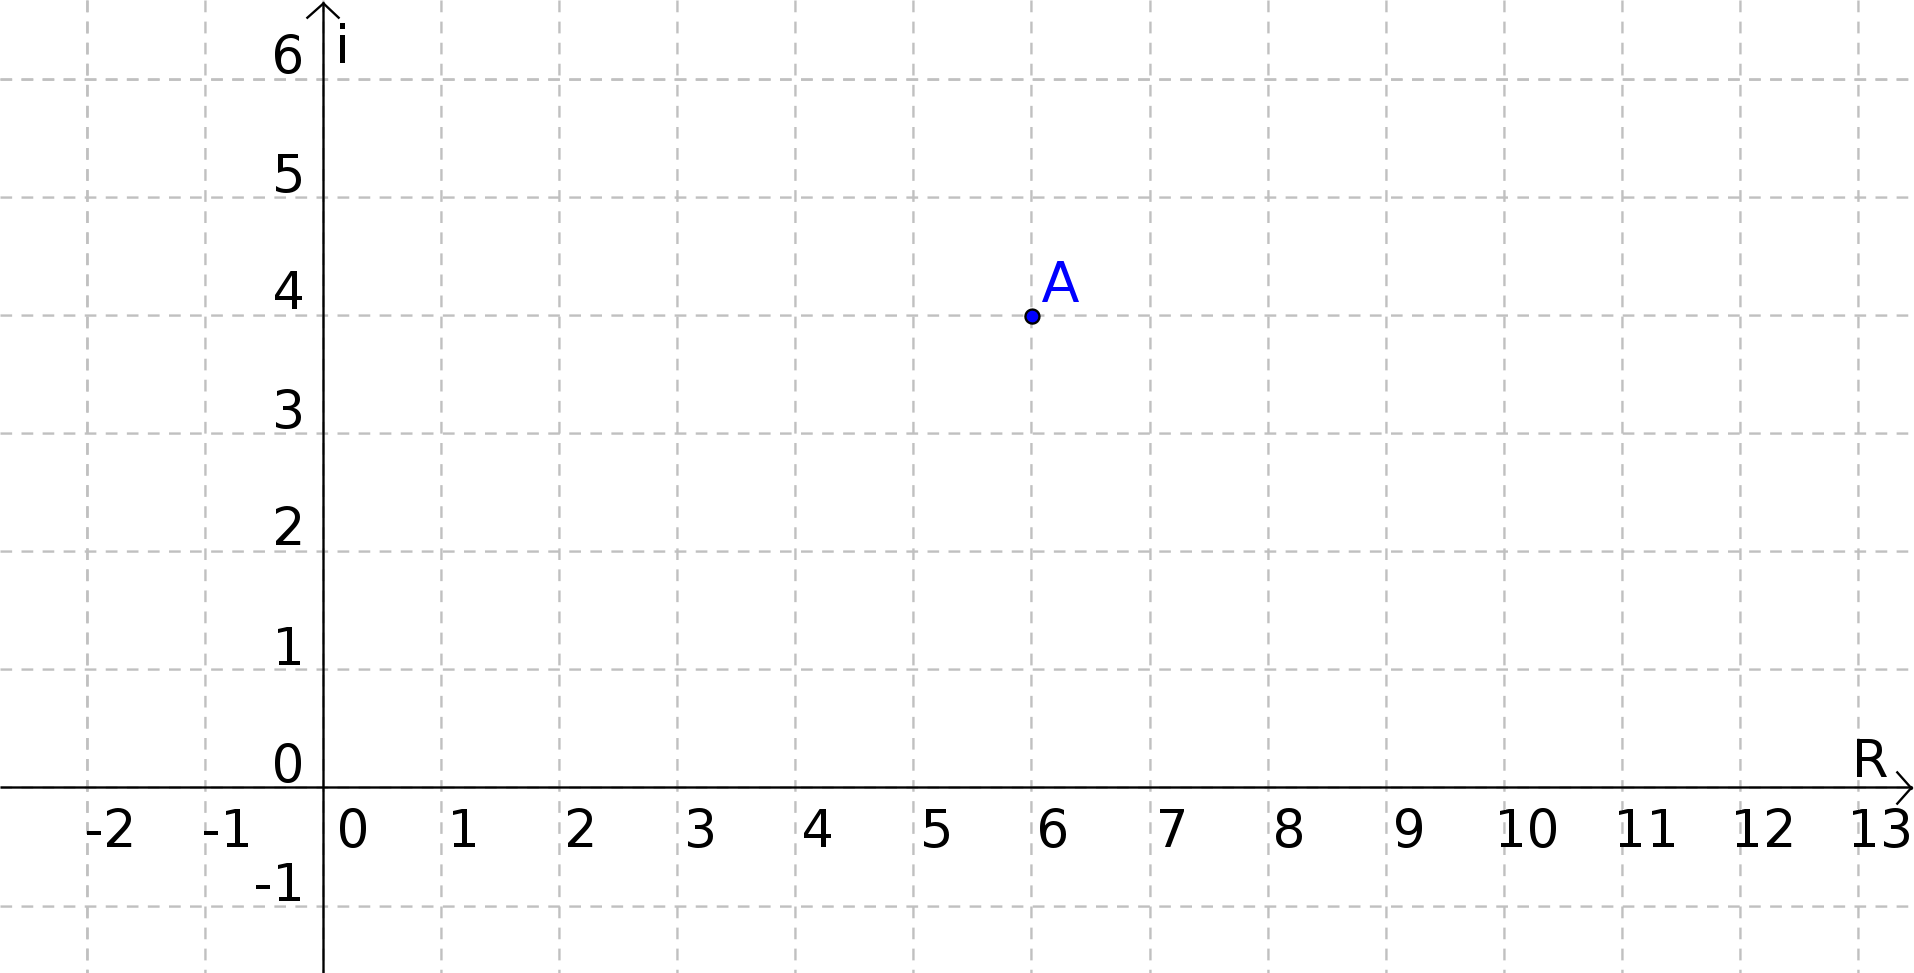
\includegraphics[width=0.5\textwidth]{Philippe/Figures_Philippe/complexes_5_1.png}
                \end{center}
            \end{question}

            \begin{reponses}
                \item[false] $6-4i$
                \item[false] $4+6i$
                \item[true] $6+4i$
                \item[false] $4-6i$
            \end{reponses}
            %%%%%%%%%%%%%%%%%%%%%%%%%%%%%%%%%%%%%

            \begin{question}{1207}{Nombres complexes}{1}{1223}
                L'impédance d'un système électrique de partie résistive $R$ et de partie réactive $X$ est $Z = R + iX$, avec $i^2=-1$. Dans quelle partie du plan complexe se situe $Z$ si $R=-2$ et $X=4$?
            \end{question}

            \begin{reponses}
                \item[false] En haut à droite.
                \item[false] En bas à droite.
                \item[false] En bas à gauche.
                \item[true] En haut à gauche.
            \end{reponses}
            %%%%%%%%%%%%%%%%%%%%%%%%%%%%%%%%%%%%%

        \subsection{Passer d'une représentation d'un nombre complexe à une autre : représentations polaire, algébrique et géométrique (calculs de modules/arguments)}
        
            \begin{question}{1208}{Nombres complexes}{2}{1208}
                Comment s'écrit $\sqrt{3}/2 + 0.5i$ en notation exponentielle?
            \end{question}

            \begin{reponses}
                \item[false] $e^{i\frac{-\pi}{3}}$
                \item[false]  $e^{i\frac{-\pi}{6}}$
                \item[true]  $e^{i\frac{\pi}{6}}$
                \item[false] $e^{i\frac{\pi}{3}}$
            \end{reponses}
            %%%%%%%%%%%%%%%%%%%%%%%%%%%%%%%%%%%%%

            \begin{question}{1208}{Nombres complexes}{2}{1208}
                Comment s'écrit l'impédance $Z=R+iX$ en notation exponentielle?
            \end{question}

            \begin{reponses}
                \item[false] $Re^{iX}$
                \item[true]  $\sqrt{R^2+X^2}\cdot e^{i\arctan(X/R)}$
                \item[false]  $\sqrt{R^2-X^2}\cdot e^{i\arctan(X/R)}$
                \item[false] $Xe^{iR}$
            \end{reponses}
            %%%%%%%%%%%%%%%%%%%%%%%%%%%%%%%%%%%%%

    \section{Calcul}
    
        \subsection{Utiliser la notation scientifique en recourant aux puissances de 10}
        
        	\begin{question}{1210}{Calcul}{1}{/}
				Comment s'écrit $3000$ en notation scientifique? 
            \end{question}

            \begin{reponses}
            	\item[false] $3\times 10^4$
            	\item[true] $3\times 10^3$
                \item[false] $3\times 10^2$
                \item[false] $3\times 10^1$
            \end{reponses}
			%%%%%%%%%%%%%%%%%%%%%%%%%%%%%%%%%%%%%
        
        	\begin{question}{1210}{Calcul}{1}{/}
				Comment s'écrit $0,003$ en notation scientifique? 
            \end{question}

            \begin{reponses}
            	\item[false] $3\times 10^{-4}$
            	\item[true] $3\times 10^{-3}$
                \item[false] $3\times 10^{-2}$
                \item[false] $3\times 10^{-1}$
            \end{reponses}
			%%%%%%%%%%%%%%%%%%%%%%%%%%%%%%%%%%%%%

        \subsection{Calculer à la main la puissance de 10 d'une application numérique (séparer les puissances de 10 des pré-facteurs qu'on calcule à part)}
        
        	\begin{question}{1211}{Calcul}{2}{/}
                Que vaut $10^{-3}\times 10^2$?
            \end{question}

            \begin{reponses}
            	\item[false] $10^{1}$
            	\item[true] $10^{-1}$
                \item[false] $10^{-5}$
                \item[false] $10^{5}$
            \end{reponses}
			%%%%%%%%%%%%%%%%%%%%%%%%%%%%%%%%%%%%%

            \begin{question}{1211}{Calcul}{2}{/}
                Que vaut $\frac{10^{-3}\times 10^{5}}{10^{4}}$?
            \end{question}

            \begin{reponses}
                \item[false] $10^{2}$
                \item[false] $10^{-6}$
                \item[false] $10^{6}$
                \item[true] $10^{-2}$
            \end{reponses}
            %%%%%%%%%%%%%%%%%%%%%%%%%%%%%%%%%%%%%
            
            \begin{question}{1211}{Calcul}{}{/}
                Que vaut $\frac{3.10^{-8}\times 2.10^{5}\times 1.10^{8}\times 7.10^{-1}\times 3.10^{-9}}{1.10^{2}\times 4.10^{-9}\times 8.10^{-9}\times 3.10^{-5}\times 1.10^{1}}$?
            \end{question}
            
            \begin{reponses}
                \item[true] $\frac{21}{16}\times 10^{15}$
                \item[false] $\frac{16}{21}\times 10^{-15}$
                \item[false] $\frac{21}{16}\times 10^{-15}$
                \item[false] $\frac{16}{21}\times 10^{15}$
            \end{reponses}
            
            \begin{question}{1211}{Calcul}{}{/}
                Que vaut $\frac{9.10^{4}\times 7.10^{-8}}{3.10^{8}\times 8.10^{-3}\times 7.10^{0}\times 2.10^{-7}}$?
            \end{question}
            
            \begin{reponses}
                \item[false] $\frac{16}{3}\times 10^{-2}$
                \item[false] $\frac{16}{3}\times 10^{2}$
                \item[false] $\frac{3}{16}\times 10^{2}$
                \item[true] $\frac{3}{16}\times 10^{-2}$
            \end{reponses}
            
            \begin{question}{1211}{Calcul}{}{/}
                Que vaut $\frac{8.10^{-6}\times 2.10^{10}\times 2.10^{6}\times 8.10^{-5}}{4.10^{10}\times 7.10^{2}\times 2.10^{-9}\times 4.10^{9}\times 5.10^{-9}}$?
            \end{question}
            
            \begin{reponses}
                \item[true] $\frac{8}{35}\times 10^{2}$
                \item[false] $\frac{35}{8}\times 10^{2}$
                \item[false] $\frac{8}{35}\times 10^{-2}$
                \item[false] $\frac{35}{8}\times 10^{-2}$
            \end{reponses}
            
            \begin{question}{1211}{Calcul}{}{/}
                Que vaut $\frac{9.10^{-10}\times 1.10^{3}\times 7.10^{-2}\times 7.10^{-1}\times 6.10^{4}}{9.10^{0}\times 1.10^{6}\times 6.10^{6}\times 6.10^{-5}\times 8.10^{-8}}$?
            \end{question}
            
            \begin{reponses}
                \item[false] $\frac{48}{49}\times 10^{5}$
                \item[true] $\frac{49}{48}\times 10^{-5}$
                \item[false] $\frac{48}{49}\times 10^{-5}$
                \item[false] $\frac{49}{48}\times 10^{5}$
            \end{reponses}
            
            \begin{question}{1211}{Calcul}{}{/}
                Que vaut $\frac{2.10^{1}}{1.10^{10}\times 9.10^{5}\times 4.10^{3}\times 2.10^{8}}$?
            \end{question}
            
            \begin{reponses}
                \item[false] $\frac{36}{1}\times 10^{25}$
                \item[false] $\frac{36}{1}\times 10^{-25}$
                \item[false] $\frac{1}{36}\times 10^{25}$
                \item[true] $\frac{1}{36}\times 10^{-25}$
            \end{reponses}
            
            \begin{question}{1211}{Calcul}{}{/}
                Que vaut $\frac{1.10^{8}\times 1.10^{3}\times 9.10^{1}}{9.10^{4}\times 5.10^{5}}$?
            \end{question}
            
            \begin{reponses}
                \item[true] $\frac{1}{5}\times 10^{3}$
                \item[false] $\frac{1}{5}\times 10^{-3}$
                \item[false] $\frac{5}{1}\times 10^{3}$
                \item[false] $\frac{5}{1}\times 10^{-3}$
            \end{reponses}
            
            \begin{question}{1211}{Calcul}{}{/}
                Que vaut $\frac{8.10^{8}}{8.10^{10}\times 4.10^{9}\times 4.10^{-10}}$?
            \end{question}
            
            \begin{reponses}
                \item[false] $\frac{1}{16}\times 10^{1}$
                \item[true] $\frac{1}{16}\times 10^{-1}$
                \item[false] $\frac{16}{1}\times 10^{-1}$
                \item[false] $\frac{16}{1}\times 10^{1}$
            \end{reponses}
            
            \begin{question}{1211}{Calcul}{}{/}
                Que vaut $\frac{9.10^{9}\times 4.10^{-5}\times 9.10^{-1}}{8.10^{-8}\times 4.10^{-8}}$?
            \end{question}
            
            \begin{reponses}
                \item[true] $\frac{81}{8}\times 10^{19}$
                \item[false] $\frac{8}{81}\times 10^{19}$
                \item[false] $\frac{8}{81}\times 10^{-19}$
                \item[false] $\frac{81}{8}\times 10^{-19}$
            \end{reponses}
            
            \begin{question}{1211}{Calcul}{}{/}
                Que vaut $\frac{1.10^{2}\times 8.10^{-7}\times 2.10^{-7}\times 4.10^{3}\times 5.10^{-4}}{4.10^{5}\times 9.10^{-4}\times 2.10^{-7}}$?
            \end{question}
            
            \begin{reponses}
                \item[true] $\frac{40}{9}\times 10^{-7}$
                \item[false] $\frac{9}{40}\times 10^{-7}$
                \item[false] $\frac{40}{9}\times 10^{7}$
                \item[false] $\frac{9}{40}\times 10^{7}$
            \end{reponses}
            
            \begin{question}{1211}{Calcul}{}{/}
                Que vaut $\frac{8.10^{7}\times 6.10^{-9}\times 5.10^{1}}{3.10^{4}\times 1.10^{8}\times 1.10^{-7}\times 5.10^{-1}}$?
            \end{question}
            
            \begin{reponses}
                \item[true] $\frac{16}{1}\times 10^{-5}$
                \item[false] $\frac{16}{1}\times 10^{5}$
                \item[false] $\frac{1}{16}\times 10^{5}$
                \item[false] $\frac{1}{16}\times 10^{-5}$
            \end{reponses}
            
            \begin{question}{1211}{Calcul}{}{/}
                Que vaut $\frac{5.10^{4}\times 5.10^{2}\times 7.10^{-5}\times 4.10^{-2}\times 6.10^{5}}{3.10^{4}\times 7.10^{4}\times 4.10^{1}\times 1.10^{0}\times 4.10^{-4}}$?
            \end{question}
            
            \begin{reponses}
                \item[false] $\frac{25}{2}\times 10^{1}$
                \item[false] $\frac{2}{25}\times 10^{-1}$
                \item[true] $\frac{25}{2}\times 10^{-1}$
                \item[false] $\frac{2}{25}\times 10^{1}$
            \end{reponses}
            
            \begin{question}{1211}{Calcul}{}{/}
                Que vaut $\frac{4.10^{10}\times 4.10^{-9}\times 3.10^{3}\times 6.10^{-5}}{2.10^{-5}\times 4.10^{9}\times 9.10^{3}\times 7.10^{0}}$?
            \end{question}
            
            \begin{reponses}
                \item[false] $\frac{7}{4}\times 10^{8}$
                \item[false] $\frac{4}{7}\times 10^{8}$
                \item[true] $\frac{4}{7}\times 10^{-8}$
                \item[false] $\frac{7}{4}\times 10^{-8}$
            \end{reponses}
            
            \begin{question}{1211}{Calcul}{}{/}
                Que vaut $\frac{3.10^{-7}\times 5.10^{7}}{1.10^{9}}$?
            \end{question}
            
            \begin{reponses}
                \item[false] $\frac{1}{15}\times 10^{9}$
                \item[false] $\frac{15}{1}\times 10^{9}$
                \item[false] $\frac{1}{15}\times 10^{-9}$
                \item[true] $\frac{15}{1}\times 10^{-9}$
            \end{reponses}
            
            \begin{question}{1211}{Calcul}{}{/}
                Que vaut $\frac{6.10^{-5}}{4.10^{5}\times 8.10^{-9}\times 7.10^{-8}}$?
            \end{question}
            
            \begin{reponses}
                \item[true] $\frac{3}{112}\times 10^{7}$
                \item[false] $\frac{112}{3}\times 10^{7}$
                \item[false] $\frac{112}{3}\times 10^{-7}$
                \item[false] $\frac{3}{112}\times 10^{-7}$
            \end{reponses}
            
            \begin{question}{1211}{Calcul}{}{/}
                Que vaut $\frac{2.10^{-4}\times 4.10^{4}}{4.10^{-9}\times 9.10^{-5}\times 9.10^{-8}\times 9.10^{2}\times 8.10^{-9}}$?
            \end{question}
            
            \begin{reponses}
                \item[false] $\frac{1}{2916}\times 10^{-29}$
                \item[true] $\frac{1}{2916}\times 10^{29}$
                \item[false] $\frac{2916}{1}\times 10^{-29}$
                \item[false] $\frac{2916}{1}\times 10^{29}$
            \end{reponses}
            
            \begin{question}{1211}{Calcul}{}{/}
                Que vaut $\frac{7.10^{0}\times 4.10^{2}\times 2.10^{-8}\times 8.10^{3}\times 4.10^{-10}}{2.10^{0}}$?
            \end{question}
            
            \begin{reponses}
                \item[false] $\frac{1}{896}\times 10^{13}$
                \item[false] $\frac{1}{896}\times 10^{-13}$
                \item[false] $\frac{896}{1}\times 10^{13}$
                \item[true] $\frac{896}{1}\times 10^{-13}$
            \end{reponses}
            
            \begin{question}{1211}{Calcul}{}{/}
                Que vaut $\frac{6.10^{2}\times 3.10^{2}}{7.10^{-3}\times 6.10^{-5}\times 3.10^{8}\times 7.10^{0}}$?
            \end{question}
            
            \begin{reponses}
                \item[true] $\frac{1}{49}\times 10^{4}$
                \item[false] $\frac{1}{49}\times 10^{-4}$
                \item[false] $\frac{49}{1}\times 10^{4}$
                \item[false] $\frac{49}{1}\times 10^{-4}$
            \end{reponses}
            
            \begin{question}{1211}{Calcul}{}{/}
                Que vaut $\frac{3.10^{5}}{9.10^{1}\times 1.10^{-1}\times 1.10^{-7}}$?
            \end{question}
            
            \begin{reponses}
                \item[false] $\frac{3}{1}\times 10^{-12}$
                \item[true] $\frac{1}{3}\times 10^{12}$
                \item[false] $\frac{3}{1}\times 10^{12}$
                \item[false] $\frac{1}{3}\times 10^{-12}$
            \end{reponses}
            
            \begin{question}{1211}{Calcul}{}{/}
                Que vaut $\frac{4.10^{-9}}{4.10^{-6}\times 5.10^{-4}\times 7.10^{-9}}$?
            \end{question}
            
            \begin{reponses}
                \item[false] $\frac{35}{1}\times 10^{-10}$
                \item[false] $\frac{1}{35}\times 10^{-10}$
                \item[true] $\frac{1}{35}\times 10^{10}$
                \item[false] $\frac{35}{1}\times 10^{10}$
            \end{reponses}
            
            \begin{question}{1211}{Calcul}{}{/}
                Que vaut $\frac{8.10^{8}}{1.10^{-10}\times 3.10^{-6}\times 9.10^{3}\times 7.10^{9}\times 7.10^{3}}$?
            \end{question}
            
            \begin{reponses}
                \item[true] $\frac{8}{1323}\times 10^{9}$
                \item[false] $\frac{1323}{8}\times 10^{9}$
                \item[false] $\frac{1323}{8}\times 10^{-9}$
                \item[false] $\frac{8}{1323}\times 10^{-9}$
            \end{reponses}
            
            \begin{question}{1211}{Calcul}{}{/}
                Que vaut $\frac{9.10^{4}}{4.10^{-4}\times 8.10^{4}\times 8.10^{-4}\times 4.10^{1}\times 3.10^{-3}}$?
            \end{question}
            
            \begin{reponses}
                \item[true] $\frac{3}{1024}\times 10^{10}$
                \item[false] $\frac{1024}{3}\times 10^{-10}$
                \item[false] $\frac{1024}{3}\times 10^{10}$
                \item[false] $\frac{3}{1024}\times 10^{-10}$
            \end{reponses}
            
            \begin{question}{1211}{Calcul}{}{/}
                Que vaut $\frac{2.10^{-10}\times 7.10^{-2}\times 2.10^{-10}\times 7.10^{1}\times 1.10^{0}}{6.10^{4}\times 6.10^{-5}\times 5.10^{-9}}$?
            \end{question}
            
            \begin{reponses}
                \item[false] $\frac{49}{45}\times 10^{11}$
                \item[true] $\frac{49}{45}\times 10^{-11}$
                \item[false] $\frac{45}{49}\times 10^{-11}$
                \item[false] $\frac{45}{49}\times 10^{11}$
            \end{reponses}
            
            \begin{question}{1211}{Calcul}{}{/}
                Que vaut $\frac{7.10^{3}\times 1.10^{-1}\times 5.10^{-8}\times 4.10^{4}}{5.10^{-1}\times 2.10^{-5}}$?
            \end{question}
            
            \begin{reponses}
                \item[false] $\frac{1}{14}\times 10^{4}$
                \item[false] $\frac{14}{1}\times 10^{-4}$
                \item[false] $\frac{1}{14}\times 10^{-4}$
                \item[true] $\frac{14}{1}\times 10^{4}$
            \end{reponses}
            
            \begin{question}{1211}{Calcul}{}{/}
                Que vaut $\frac{5.10^{2}\times 2.10^{-9}}{1.10^{2}\times 4.10^{0}\times 1.10^{-8}\times 4.10^{-4}}$?
            \end{question}
            
            \begin{reponses}
                \item[false] $\frac{5}{8}\times 10^{-3}$
                \item[false] $\frac{8}{5}\times 10^{-3}$
                \item[false] $\frac{8}{5}\times 10^{3}$
                \item[true] $\frac{5}{8}\times 10^{3}$
            \end{reponses}
            
            \begin{question}{1211}{Calcul}{}{/}
                Que vaut $\frac{2.10^{4}\times 8.10^{2}\times 9.10^{-9}\times 2.10^{2}\times 3.10^{3}}{5.10^{3}\times 3.10^{-8}}$?
            \end{question}
            
            \begin{reponses}
                \item[false] $\frac{5}{288}\times 10^{7}$
                \item[false] $\frac{288}{5}\times 10^{-7}$
                \item[true] $\frac{288}{5}\times 10^{7}$
                \item[false] $\frac{5}{288}\times 10^{-7}$
            \end{reponses}
            
            \begin{question}{1211}{Calcul}{}{/}
                Que vaut $\frac{5.10^{2}\times 6.10^{-4}}{4.10^{6}\times 2.10^{8}\times 2.10^{-10}\times 3.10^{-10}\times 8.10^{5}}$?
            \end{question}
            
            \begin{reponses}
                \item[false] $\frac{5}{64}\times 10^{1}$
                \item[false] $\frac{64}{5}\times 10^{1}$
                \item[true] $\frac{5}{64}\times 10^{-1}$
                \item[false] $\frac{64}{5}\times 10^{-1}$
            \end{reponses}
            
            \begin{question}{1211}{Calcul}{}{/}
                Que vaut $\frac{5.10^{-8}}{7.10^{0}\times 2.10^{-1}\times 7.10^{2}\times 4.10^{-5}}$?
            \end{question}
            
            \begin{reponses}
                \item[false] $\frac{392}{5}\times 10^{-4}$
                \item[true] $\frac{5}{392}\times 10^{-4}$
                \item[false] $\frac{392}{5}\times 10^{4}$
                \item[false] $\frac{5}{392}\times 10^{4}$
            \end{reponses}
            
            \begin{question}{1211}{Calcul}{}{/}
                Que vaut $\frac{9.10^{5}\times 8.10^{-1}\times 1.10^{-8}\times 7.10^{-5}}{8.10^{2}\times 5.10^{8}\times 4.10^{-7}}$?
            \end{question}
            
            \begin{reponses}
                \item[false] $\frac{20}{63}\times 10^{-12}$
                \item[false] $\frac{63}{20}\times 10^{12}$
                \item[true] $\frac{63}{20}\times 10^{-12}$
                \item[false] $\frac{20}{63}\times 10^{12}$
            \end{reponses}
            
            \begin{question}{1211}{Calcul}{}{/}
                Que vaut $\frac{2.10^{2}}{3.10^{4}\times 1.10^{6}\times 4.10^{10}\times 6.10^{3}}$?
            \end{question}
            
            \begin{reponses}
                \item[false] $\frac{36}{1}\times 10^{-21}$
                \item[false] $\frac{1}{36}\times 10^{21}$
                \item[false] $\frac{36}{1}\times 10^{21}$
                \item[true] $\frac{1}{36}\times 10^{-21}$
            \end{reponses}
            
            \begin{question}{1211}{Calcul}{}{/}
                Que vaut $\frac{4.10^{-9}\times 1.10^{-10}\times 5.10^{8}\times 2.10^{-3}}{3.10^{1}\times 7.10^{9}\times 1.10^{3}\times 5.10^{1}\times 6.10^{-9}}$?
            \end{question}
            
            \begin{reponses}
                \item[false] $\frac{63}{4}\times 10^{19}$
                \item[true] $\frac{4}{63}\times 10^{-19}$
                \item[false] $\frac{4}{63}\times 10^{19}$
                \item[false] $\frac{63}{4}\times 10^{-19}$
            \end{reponses}
            
            \begin{question}{1211}{Calcul}{}{/}
                Que vaut $\frac{4.10^{9}\times 5.10^{4}\times 8.10^{3}}{4.10^{4}\times 6.10^{2}\times 5.10^{-4}\times 6.10^{10}}$?
            \end{question}
            
            \begin{reponses}
                \item[false] $\frac{9}{2}\times 10^{4}$
                \item[false] $\frac{2}{9}\times 10^{-4}$
                \item[false] $\frac{9}{2}\times 10^{-4}$
                \item[true] $\frac{2}{9}\times 10^{4}$
            \end{reponses}
            
            \begin{question}{1211}{Calcul}{}{/}
                Que vaut $\frac{6.10^{10}}{2.10^{2}\times 8.10^{-2}\times 5.10^{6}}$?
            \end{question}
            
            \begin{reponses}
                \item[false] $\frac{3}{40}\times 10^{-4}$
                \item[true] $\frac{3}{40}\times 10^{4}$
                \item[false] $\frac{40}{3}\times 10^{-4}$
                \item[false] $\frac{40}{3}\times 10^{4}$
            \end{reponses}
            
            \begin{question}{1211}{Calcul}{}{/}
                Que vaut $\frac{2.10^{10}\times 5.10^{2}\times 6.10^{-10}}{5.10^{-2}\times 7.10^{-5}}$?
            \end{question}
            
            \begin{reponses}
                \item[false] $\frac{12}{7}\times 10^{-9}$
                \item[true] $\frac{12}{7}\times 10^{9}$
                \item[false] $\frac{7}{12}\times 10^{-9}$
                \item[false] $\frac{7}{12}\times 10^{9}$
            \end{reponses}
            
            \begin{question}{1211}{Calcul}{}{/}
                Que vaut $\frac{1.10^{-6}\times 8.10^{1}\times 3.10^{-9}\times 3.10^{8}}{9.10^{-1}}$?
            \end{question}
            
            \begin{reponses}
                \item[false] $\frac{8}{1}\times 10^{5}$
                \item[true] $\frac{8}{1}\times 10^{-5}$
                \item[false] $\frac{1}{8}\times 10^{5}$
                \item[false] $\frac{1}{8}\times 10^{-5}$
            \end{reponses}
            
            \begin{question}{1211}{Calcul}{}{/}
                Que vaut $\frac{8.10^{6}\times 7.10^{-7}\times 7.10^{0}}{5.10^{2}\times 4.10^{4}}$?
            \end{question}
            
            \begin{reponses}
                \item[false] $\frac{5}{98}\times 10^{-7}$
                \item[false] $\frac{98}{5}\times 10^{7}$
                \item[false] $\frac{5}{98}\times 10^{7}$
                \item[true] $\frac{98}{5}\times 10^{-7}$
            \end{reponses}
            
            \begin{question}{1211}{Calcul}{}{/}
                Que vaut $\frac{2.10^{6}\times 4.10^{0}}{2.10^{1}\times 2.10^{-3}\times 2.10^{-3}\times 1.10^{5}\times 8.10^{10}}$?
            \end{question}
            
            \begin{reponses}
                \item[false] $\frac{8}{1}\times 10^{4}$
                \item[false] $\frac{8}{1}\times 10^{-4}$
                \item[false] $\frac{1}{8}\times 10^{4}$
                \item[true] $\frac{1}{8}\times 10^{-4}$
            \end{reponses}
            
            \begin{question}{1211}{Calcul}{}{/}
                Que vaut $\frac{2.10^{6}}{6.10^{3}}$?
            \end{question}
            
            \begin{reponses}
                \item[false] $\frac{3}{1}\times 10^{3}$
                \item[false] $\frac{1}{3}\times 10^{-3}$
                \item[true] $\frac{1}{3}\times 10^{3}$
                \item[false] $\frac{3}{1}\times 10^{-3}$
            \end{reponses}
            
            \begin{question}{1211}{Calcul}{}{/}
                Que vaut $\frac{4.10^{4}}{7.10^{5}\times 9.10^{2}\times 6.10^{6}\times 6.10^{2}}$?
            \end{question}
            
            \begin{reponses}
                \item[false] $\frac{1}{567}\times 10^{11}$
                \item[true] $\frac{1}{567}\times 10^{-11}$
                \item[false] $\frac{567}{1}\times 10^{11}$
                \item[false] $\frac{567}{1}\times 10^{-11}$
            \end{reponses}
            
            \begin{question}{1211}{Calcul}{}{/}
                Que vaut $\frac{4.10^{-1}\times 5.10^{-3}\times 2.10^{9}\times 5.10^{4}\times 6.10^{3}}{4.10^{-9}\times 2.10^{-2}\times 2.10^{-10}\times 5.10^{6}}$?
            \end{question}
            
            \begin{reponses}
                \item[false] $\frac{1}{15}\times 10^{27}$
                \item[false] $\frac{1}{15}\times 10^{-27}$
                \item[false] $\frac{15}{1}\times 10^{-27}$
                \item[true] $\frac{15}{1}\times 10^{27}$
            \end{reponses}
            
            \begin{question}{1211}{Calcul}{}{/}
                Que vaut $\frac{4.10^{-2}\times 4.10^{-1}\times 1.10^{5}\times 5.10^{0}\times 3.10^{-6}}{4.10^{6}\times 8.10^{4}\times 3.10^{-2}}$?
            \end{question}
            
            \begin{reponses}
                \item[false] $\frac{2}{5}\times 10^{-12}$
                \item[false] $\frac{2}{5}\times 10^{12}$
                \item[false] $\frac{5}{2}\times 10^{12}$
                \item[true] $\frac{5}{2}\times 10^{-12}$
            \end{reponses}
            
            \begin{question}{1211}{Calcul}{}{/}
                Que vaut $\frac{9.10^{9}\times 6.10^{6}}{3.10^{1}}$?
            \end{question}
            
            \begin{reponses}
                \item[false] $\frac{18}{1}\times 10^{-14}$
                \item[false] $\frac{1}{18}\times 10^{14}$
                \item[false] $\frac{1}{18}\times 10^{-14}$
                \item[true] $\frac{18}{1}\times 10^{14}$
            \end{reponses}
            
            \begin{question}{1211}{Calcul}{}{/}
                Que vaut $\frac{3.10^{-2}\times 9.10^{-2}}{4.10^{10}\times 5.10^{2}\times 9.10^{0}}$?
            \end{question}
            
            \begin{reponses}
                \item[false] $\frac{20}{3}\times 10^{-16}$
                \item[true] $\frac{3}{20}\times 10^{-16}$
                \item[false] $\frac{20}{3}\times 10^{16}$
                \item[false] $\frac{3}{20}\times 10^{16}$
            \end{reponses}
            
            \begin{question}{1211}{Calcul}{}{/}
                Que vaut $\frac{8.10^{7}\times 3.10^{-3}\times 4.10^{-5}\times 9.10^{-2}}{7.10^{4}\times 9.10^{-8}\times 3.10^{-5}\times 6.10^{4}}$?
            \end{question}
            
            \begin{reponses}
                \item[false] $\frac{16}{21}\times 10^{-2}$
                \item[false] $\frac{21}{16}\times 10^{-2}$
                \item[false] $\frac{21}{16}\times 10^{2}$
                \item[true] $\frac{16}{21}\times 10^{2}$
            \end{reponses}
            
            \begin{question}{1211}{Calcul}{}{/}
                Que vaut $\frac{8.10^{-6}\times 4.10^{9}\times 5.10^{-10}\times 9.10^{-9}}{2.10^{-2}\times 8.10^{0}}$?
            \end{question}
            
            \begin{reponses}
                \item[false] $\frac{1}{90}\times 10^{14}$
                \item[false] $\frac{90}{1}\times 10^{14}$
                \item[true] $\frac{90}{1}\times 10^{-14}$
                \item[false] $\frac{1}{90}\times 10^{-14}$
            \end{reponses}
            
            \begin{question}{1211}{Calcul}{}{/}
                Que vaut $\frac{4.10^{-7}\times 2.10^{7}\times 9.10^{8}\times 9.10^{0}}{7.10^{4}}$?
            \end{question}
            
            \begin{reponses}
                \item[false] $\frac{648}{7}\times 10^{-4}$
                \item[false] $\frac{7}{648}\times 10^{4}$
                \item[false] $\frac{7}{648}\times 10^{-4}$
                \item[true] $\frac{648}{7}\times 10^{4}$
            \end{reponses}
            
            \begin{question}{1211}{Calcul}{}{/}
                Que vaut $\frac{4.10^{-10}}{5.10^{5}}$?
            \end{question}
            
            \begin{reponses}
                \item[true] $\frac{4}{5}\times 10^{-15}$
                \item[false] $\frac{4}{5}\times 10^{15}$
                \item[false] $\frac{5}{4}\times 10^{-15}$
                \item[false] $\frac{5}{4}\times 10^{15}$
            \end{reponses}
            
            \begin{question}{1211}{Calcul}{}{/}
                Que vaut $\frac{6.10^{-9}\times 1.10^{-9}}{4.10^{9}\times 4.10^{1}\times 5.10^{-10}}$?
            \end{question}
            
            \begin{reponses}
                \item[true] $\frac{3}{40}\times 10^{-18}$
                \item[false] $\frac{40}{3}\times 10^{-18}$
                \item[false] $\frac{40}{3}\times 10^{18}$
                \item[false] $\frac{3}{40}\times 10^{18}$
            \end{reponses}
            
            \begin{question}{1211}{Calcul}{}{/}
                Que vaut $\frac{7.10^{5}\times 2.10^{0}}{1.10^{2}}$?
            \end{question}
            
            \begin{reponses}
                \item[false] $\frac{14}{1}\times 10^{-3}$
                \item[false] $\frac{1}{14}\times 10^{3}$
                \item[true] $\frac{14}{1}\times 10^{3}$
                \item[false] $\frac{1}{14}\times 10^{-3}$
            \end{reponses}
            
            \begin{question}{1211}{Calcul}{}{/}
                Que vaut $\frac{3.10^{-3}\times 7.10^{3}\times 8.10^{2}}{8.10^{8}\times 2.10^{-10}\times 3.10^{-10}\times 1.10^{-4}\times 6.10^{-4}}$?
            \end{question}
            
            \begin{reponses}
                \item[true] $\frac{7}{12}\times 10^{22}$
                \item[false] $\frac{7}{12}\times 10^{-22}$
                \item[false] $\frac{12}{7}\times 10^{-22}$
                \item[false] $\frac{12}{7}\times 10^{22}$
            \end{reponses}
            
            \begin{question}{1211}{Calcul}{}{/}
                Que vaut $\frac{5.10^{10}\times 2.10^{0}\times 7.10^{-1}}{4.10^{4}\times 2.10^{-10}}$?
            \end{question}
            
            \begin{reponses}
                \item[false] $\frac{4}{35}\times 10^{-15}$
                \item[false] $\frac{35}{4}\times 10^{-15}$
                \item[true] $\frac{35}{4}\times 10^{15}$
                \item[false] $\frac{4}{35}\times 10^{15}$
            \end{reponses}
            
            \begin{question}{1211}{Calcul}{}{/}
                Que vaut $\frac{4.10^{6}\times 8.10^{5}\times 4.10^{1}\times 4.10^{-8}}{2.10^{8}\times 2.10^{8}}$?
            \end{question}
            
            \begin{reponses}
                \item[false] $\frac{1}{128}\times 10^{12}$
                \item[false] $\frac{1}{128}\times 10^{-12}$
                \item[true] $\frac{128}{1}\times 10^{-12}$
                \item[false] $\frac{128}{1}\times 10^{12}$
            \end{reponses}
            
            \begin{question}{1211}{Calcul}{}{/}
                Que vaut $\frac{3.10^{-5}\times 3.10^{2}\times 6.10^{-1}\times 2.10^{1}\times 7.10^{-1}}{3.10^{-9}}$?
            \end{question}
            
            \begin{reponses}
                \item[false] $\frac{1}{252}\times 10^{5}$
                \item[false] $\frac{252}{1}\times 10^{-5}$
                \item[false] $\frac{1}{252}\times 10^{-5}$
                \item[true] $\frac{252}{1}\times 10^{5}$
            \end{reponses}
            
            \begin{question}{1211}{Calcul}{}{/}
                Que vaut $\frac{2.10^{-7}\times 8.10^{-7}\times 7.10^{3}\times 9.10^{-5}\times 4.10^{8}}{2.10^{1}\times 2.10^{6}\times 9.10^{4}}$?
            \end{question}
            
            \begin{reponses}
                \item[false] $\frac{112}{1}\times 10^{19}$
                \item[false] $\frac{1}{112}\times 10^{19}$
                \item[false] $\frac{1}{112}\times 10^{-19}$
                \item[true] $\frac{112}{1}\times 10^{-19}$
            \end{reponses}
            
            \begin{question}{1211}{Calcul}{}{/}
                Que vaut $\frac{8.10^{-10}}{5.10^{4}\times 4.10^{10}\times 8.10^{0}\times 2.10^{-6}}$?
            \end{question}
            
            \begin{reponses}
                \item[true] $\frac{1}{40}\times 10^{-18}$
                \item[false] $\frac{40}{1}\times 10^{18}$
                \item[false] $\frac{1}{40}\times 10^{18}$
                \item[false] $\frac{40}{1}\times 10^{-18}$
            \end{reponses}
            
            \begin{question}{1211}{Calcul}{}{/}
                Que vaut $\frac{5.10^{3}\times 3.10^{9}}{1.10^{2}\times 5.10^{0}\times 4.10^{4}\times 7.10^{0}}$?
            \end{question}
            
            \begin{reponses}
                \item[false] $\frac{28}{3}\times 10^{6}$
                \item[false] $\frac{3}{28}\times 10^{-6}$
                \item[false] $\frac{28}{3}\times 10^{-6}$
                \item[true] $\frac{3}{28}\times 10^{6}$
            \end{reponses}
            
            \begin{question}{1211}{Calcul}{}{/}
                Que vaut $\frac{3.10^{5}\times 7.10^{8}}{3.10^{3}\times 8.10^{4}\times 4.10^{6}\times 3.10^{1}}$?
            \end{question}
            
            \begin{reponses}
                \item[false] $\frac{96}{7}\times 10^{-1}$
                \item[true] $\frac{7}{96}\times 10^{-1}$
                \item[false] $\frac{96}{7}\times 10^{1}$
                \item[false] $\frac{7}{96}\times 10^{1}$
            \end{reponses}
            
            \begin{question}{1211}{Calcul}{}{/}
                Que vaut $\frac{7.10^{-7}\times 5.10^{0}}{3.10^{-8}\times 6.10^{-9}\times 1.10^{10}}$?
            \end{question}
            
            \begin{reponses}
                \item[false] $\frac{18}{35}\times 10^{0}$
                \item[false] $\frac{18}{35}\times 10^{0}$
                \item[true] $\frac{35}{18}\times 10^{0}$
                \item[false] $\frac{35}{18}\times 10^{0}$
            \end{reponses}
            
            \begin{question}{1211}{Calcul}{}{/}
                Que vaut $\frac{2.10^{4}}{5.10^{-5}}$?
            \end{question}
            
            \begin{reponses}
                \item[false] $\frac{5}{2}\times 10^{9}$
                \item[false] $\frac{2}{5}\times 10^{-9}$
                \item[true] $\frac{2}{5}\times 10^{9}$
                \item[false] $\frac{5}{2}\times 10^{-9}$
            \end{reponses}
            
            \begin{question}{1211}{Calcul}{}{/}
                Que vaut $\frac{2.10^{2}\times 2.10^{-4}}{2.10^{7}\times 8.10^{6}\times 3.10^{0}}$?
            \end{question}
            
            \begin{reponses}
                \item[true] $\frac{1}{12}\times 10^{-15}$
                \item[false] $\frac{12}{1}\times 10^{15}$
                \item[false] $\frac{1}{12}\times 10^{15}$
                \item[false] $\frac{12}{1}\times 10^{-15}$
            \end{reponses}
            
            \begin{question}{1211}{Calcul}{}{/}
                Que vaut $\frac{4.10^{-7}\times 2.10^{-2}}{5.10^{1}}$?
            \end{question}
            
            \begin{reponses}
                \item[false] $\frac{8}{5}\times 10^{10}$
                \item[false] $\frac{5}{8}\times 10^{10}$
                \item[true] $\frac{8}{5}\times 10^{-10}$
                \item[false] $\frac{5}{8}\times 10^{-10}$
            \end{reponses}
            
            \begin{question}{1211}{Calcul}{}{/}
                Que vaut $\frac{3.10^{10}\times 4.10^{-6}\times 6.10^{5}\times 8.10^{3}\times 8.10^{1}}{4.10^{7}\times 8.10^{1}}$?
            \end{question}
            
            \begin{reponses}
                \item[false] $\frac{1}{144}\times 10^{5}$
                \item[false] $\frac{1}{144}\times 10^{-5}$
                \item[true] $\frac{144}{1}\times 10^{5}$
                \item[false] $\frac{144}{1}\times 10^{-5}$
            \end{reponses}
            
            \begin{question}{1211}{Calcul}{}{/}
                Que vaut $\frac{8.10^{4}}{8.10^{6}\times 3.10^{-6}\times 5.10^{-1}\times 1.10^{3}\times 3.10^{7}}$?
            \end{question}
            
            \begin{reponses}
                \item[false] $\frac{45}{1}\times 10^{5}$
                \item[false] $\frac{45}{1}\times 10^{-5}$
                \item[false] $\frac{1}{45}\times 10^{5}$
                \item[true] $\frac{1}{45}\times 10^{-5}$
            \end{reponses}
            
            \begin{question}{1211}{Calcul}{}{/}
                Que vaut $\frac{7.10^{-6}\times 9.10^{7}\times 7.10^{-5}\times 3.10^{0}\times 7.10^{-8}}{8.10^{-2}\times 8.10^{-2}\times 8.10^{-10}\times 3.10^{-9}}$?
            \end{question}
            
            \begin{reponses}
                \item[false] $\frac{512}{3087}\times 10^{11}$
                \item[false] $\frac{3087}{512}\times 10^{-11}$
                \item[true] $\frac{3087}{512}\times 10^{11}$
                \item[false] $\frac{512}{3087}\times 10^{-11}$
            \end{reponses}
            
            \begin{question}{1211}{Calcul}{}{/}
                Que vaut $\frac{9.10^{4}\times 6.10^{-9}\times 4.10^{9}\times 2.10^{-4}}{9.10^{-5}}$?
            \end{question}
            
            \begin{reponses}
                \item[false] $\frac{48}{1}\times 10^{-5}$
                \item[false] $\frac{1}{48}\times 10^{5}$
                \item[false] $\frac{1}{48}\times 10^{-5}$
                \item[true] $\frac{48}{1}\times 10^{5}$
            \end{reponses}
            
            \begin{question}{1211}{Calcul}{}{/}
                Que vaut $\frac{5.10^{6}\times 4.10^{8}}{7.10^{-10}\times 3.10^{-8}\times 7.10^{-8}\times 6.10^{-9}\times 6.10^{8}}$?
            \end{question}
            
            \begin{reponses}
                \item[false] $\frac{5}{1323}\times 10^{-41}$
                \item[false] $\frac{1323}{5}\times 10^{41}$
                \item[true] $\frac{5}{1323}\times 10^{41}$
                \item[false] $\frac{1323}{5}\times 10^{-41}$
            \end{reponses}
            
            \begin{question}{1211}{Calcul}{}{/}
                Que vaut $\frac{2.10^{-10}}{6.10^{-5}\times 1.10^{3}}$?
            \end{question}
            
            \begin{reponses}
                \item[false] $\frac{3}{1}\times 10^{8}$
                \item[false] $\frac{3}{1}\times 10^{-8}$
                \item[true] $\frac{1}{3}\times 10^{-8}$
                \item[false] $\frac{1}{3}\times 10^{8}$
            \end{reponses}
            
            \begin{question}{1211}{Calcul}{}{/}
                Que vaut $\frac{9.10^{3}\times 1.10^{0}\times 1.10^{-8}}{4.10^{-10}\times 6.10^{6}\times 2.10^{-1}}$?
            \end{question}
            
            \begin{reponses}
                \item[false] $\frac{16}{3}\times 10^{0}$
                \item[false] $\frac{3}{16}\times 10^{0}$
                \item[true] $\frac{3}{16}\times 10^{0}$
                \item[false] $\frac{16}{3}\times 10^{0}$
            \end{reponses}
            
            \begin{question}{1211}{Calcul}{}{/}
                Que vaut $\frac{1.10^{2}\times 8.10^{-5}\times 8.10^{4}}{5.10^{3}}$?
            \end{question}
            
            \begin{reponses}
                \item[false] $\frac{5}{64}\times 10^{-2}$
                \item[false] $\frac{5}{64}\times 10^{2}$
                \item[true] $\frac{64}{5}\times 10^{-2}$
                \item[false] $\frac{64}{5}\times 10^{2}$
            \end{reponses}
            
            \begin{question}{1211}{Calcul}{}{/}
                Que vaut $\frac{7.10^{5}\times 5.10^{0}\times 1.10^{5}}{3.10^{9}\times 4.10^{2}\times 6.10^{-2}\times 8.10^{8}}$?
            \end{question}
            
            \begin{reponses}
                \item[false] $\frac{576}{35}\times 10^{-7}$
                \item[false] $\frac{576}{35}\times 10^{7}$
                \item[false] $\frac{35}{576}\times 10^{7}$
                \item[true] $\frac{35}{576}\times 10^{-7}$
            \end{reponses}
            
            \begin{question}{1211}{Calcul}{}{/}
                Que vaut $\frac{5.10^{3}\times 4.10^{3}\times 9.10^{4}\times 8.10^{3}\times 5.10^{5}}{2.10^{1}\times 4.10^{-8}\times 8.10^{-10}\times 6.10^{-3}\times 1.10^{-4}}$?
            \end{question}
            
            \begin{reponses}
                \item[false] $\frac{75}{4}\times 10^{-42}$
                \item[false] $\frac{4}{75}\times 10^{42}$
                \item[true] $\frac{75}{4}\times 10^{42}$
                \item[false] $\frac{4}{75}\times 10^{-42}$
            \end{reponses}
            
            \begin{question}{1211}{Calcul}{}{/}
                Que vaut $\frac{2.10^{10}\times 9.10^{-6}\times 6.10^{0}}{8.10^{-6}}$?
            \end{question}
            
            \begin{reponses}
                \item[false] $\frac{2}{27}\times 10^{-10}$
                \item[false] $\frac{27}{2}\times 10^{-10}$
                \item[false] $\frac{2}{27}\times 10^{10}$
                \item[true] $\frac{27}{2}\times 10^{10}$
            \end{reponses}
            
            \begin{question}{1211}{Calcul}{}{/}
                Que vaut $\frac{8.10^{-8}\times 9.10^{-2}}{2.10^{-1}\times 6.10^{7}\times 5.10^{4}\times 1.10^{6}\times 4.10^{9}}$?
            \end{question}
            
            \begin{reponses}
                \item[false] $\frac{3}{10}\times 10^{35}$
                \item[false] $\frac{10}{3}\times 10^{35}$
                \item[false] $\frac{10}{3}\times 10^{-35}$
                \item[true] $\frac{3}{10}\times 10^{-35}$
            \end{reponses}
            
            \begin{question}{1211}{Calcul}{}{/}
                Que vaut $\frac{8.10^{4}\times 5.10^{-3}\times 6.10^{7}}{2.10^{1}\times 2.10^{7}\times 5.10^{7}\times 5.10^{7}\times 6.10^{0}}$?
            \end{question}
            
            \begin{reponses}
                \item[true] $\frac{2}{5}\times 10^{-14}$
                \item[false] $\frac{2}{5}\times 10^{14}$
                \item[false] $\frac{5}{2}\times 10^{-14}$
                \item[false] $\frac{5}{2}\times 10^{14}$
            \end{reponses}
            
            \begin{question}{1211}{Calcul}{}{/}
                Que vaut $\frac{6.10^{0}\times 9.10^{0}\times 9.10^{-2}}{6.10^{2}}$?
            \end{question}
            
            \begin{reponses}
                \item[false] $\frac{81}{1}\times 10^{4}$
                \item[false] $\frac{1}{81}\times 10^{4}$
                \item[true] $\frac{81}{1}\times 10^{-4}$
                \item[false] $\frac{1}{81}\times 10^{-4}$
            \end{reponses}
            
            \begin{question}{1211}{Calcul}{}{/}
                Que vaut $\frac{1.10^{-8}}{4.10^{-3}\times 9.10^{-8}\times 1.10^{-6}\times 6.10^{3}\times 3.10^{9}}$?
            \end{question}
            
            \begin{reponses}
                \item[false] $\frac{1}{648}\times 10^{3}$
                \item[true] $\frac{1}{648}\times 10^{-3}$
                \item[false] $\frac{648}{1}\times 10^{-3}$
                \item[false] $\frac{648}{1}\times 10^{3}$
            \end{reponses}
            
            \begin{question}{1211}{Calcul}{}{/}
                Que vaut $\frac{2.10^{-7}\times 3.10^{-5}\times 9.10^{0}}{9.10^{-1}\times 6.10^{-1}\times 6.10^{-3}\times 4.10^{9}\times 1.10^{3}}$?
            \end{question}
            
            \begin{reponses}
                \item[false] $\frac{24}{1}\times 10^{-19}$
                \item[false] $\frac{1}{24}\times 10^{19}$
                \item[false] $\frac{24}{1}\times 10^{19}$
                \item[true] $\frac{1}{24}\times 10^{-19}$
            \end{reponses}
            
            \begin{question}{1211}{Calcul}{}{/}
                Que vaut $\frac{8.10^{4}\times 6.10^{2}\times 4.10^{6}\times 6.10^{-6}}{3.10^{3}\times 5.10^{-8}\times 9.10^{-8}}$?
            \end{question}
            
            \begin{reponses}
                \item[true] $\frac{128}{15}\times 10^{19}$
                \item[false] $\frac{15}{128}\times 10^{19}$
                \item[false] $\frac{128}{15}\times 10^{-19}$
                \item[false] $\frac{15}{128}\times 10^{-19}$
            \end{reponses}
            
            \begin{question}{1211}{Calcul}{}{/}
                Que vaut $\frac{5.10^{10}\times 6.10^{5}\times 8.10^{4}\times 3.10^{0}}{1.10^{3}\times 5.10^{-10}\times 6.10^{6}\times 8.10^{8}}$?
            \end{question}
            
            \begin{reponses}
                \item[false] $\frac{3}{1}\times 10^{-12}$
                \item[false] $\frac{1}{3}\times 10^{-12}$
                \item[true] $\frac{3}{1}\times 10^{12}$
                \item[false] $\frac{1}{3}\times 10^{12}$
            \end{reponses}
            
            \begin{question}{1211}{Calcul}{}{/}
                Que vaut $\frac{2.10^{6}}{9.10^{2}\times 3.10^{-7}\times 1.10^{-4}\times 5.10^{2}\times 4.10^{-10}}$?
            \end{question}
            
            \begin{reponses}
                \item[false] $\frac{1}{270}\times 10^{-23}$
                \item[true] $\frac{1}{270}\times 10^{23}$
                \item[false] $\frac{270}{1}\times 10^{23}$
                \item[false] $\frac{270}{1}\times 10^{-23}$
            \end{reponses}
            
            \begin{question}{1211}{Calcul}{}{/}
                Que vaut $\frac{1.10^{-6}\times 8.10^{8}\times 3.10^{-10}}{2.10^{3}}$?
            \end{question}
            
            \begin{reponses}
                \item[true] $\frac{12}{1}\times 10^{-11}$
                \item[false] $\frac{1}{12}\times 10^{11}$
                \item[false] $\frac{1}{12}\times 10^{-11}$
                \item[false] $\frac{12}{1}\times 10^{11}$
            \end{reponses}
            
            \begin{question}{1211}{Calcul}{}{/}
                Que vaut $\frac{9.10^{0}\times 5.10^{3}\times 1.10^{6}\times 8.10^{7}\times 5.10^{7}}{4.10^{7}\times 7.10^{-5}\times 3.10^{9}}$?
            \end{question}
            
            \begin{reponses}
                \item[false] $\frac{7}{150}\times 10^{12}$
                \item[false] $\frac{7}{150}\times 10^{-12}$
                \item[false] $\frac{150}{7}\times 10^{-12}$
                \item[true] $\frac{150}{7}\times 10^{12}$
            \end{reponses}
            
            \begin{question}{1211}{Calcul}{}{/}
                Que vaut $\frac{5.10^{0}\times 2.10^{2}}{1.10^{7}\times 3.10^{7}\times 6.10^{-6}}$?
            \end{question}
            
            \begin{reponses}
                \item[false] $\frac{9}{5}\times 10^{6}$
                \item[false] $\frac{5}{9}\times 10^{6}$
                \item[true] $\frac{5}{9}\times 10^{-6}$
                \item[false] $\frac{9}{5}\times 10^{-6}$
            \end{reponses}
            
            \begin{question}{1211}{Calcul}{}{/}
                Que vaut $\frac{9.10^{9}\times 2.10^{-9}\times 3.10^{10}}{1.10^{-2}}$?
            \end{question}
            
            \begin{reponses}
                \item[false] $\frac{54}{1}\times 10^{-12}$
                \item[false] $\frac{1}{54}\times 10^{12}$
                \item[false] $\frac{1}{54}\times 10^{-12}$
                \item[true] $\frac{54}{1}\times 10^{12}$
            \end{reponses}
            
            \begin{question}{1211}{Calcul}{}{/}
                Que vaut $\frac{1.10^{-1}\times 5.10^{-9}\times 1.10^{6}}{2.10^{-3}}$?
            \end{question}
            
            \begin{reponses}
                \item[true] $\frac{5}{2}\times 10^{-1}$
                \item[false] $\frac{5}{2}\times 10^{1}$
                \item[false] $\frac{2}{5}\times 10^{-1}$
                \item[false] $\frac{2}{5}\times 10^{1}$
            \end{reponses}
            
            \begin{question}{1211}{Calcul}{}{/}
                Que vaut $\frac{1.10^{-7}\times 2.10^{-6}\times 6.10^{9}\times 8.10^{1}}{7.10^{-2}}$?
            \end{question}
            
            \begin{reponses}
                \item[true] $\frac{96}{7}\times 10^{-1}$
                \item[false] $\frac{96}{7}\times 10^{1}$
                \item[false] $\frac{7}{96}\times 10^{-1}$
                \item[false] $\frac{7}{96}\times 10^{1}$
            \end{reponses}
            
            \begin{question}{1211}{Calcul}{}{/}
                Que vaut $\frac{6.10^{-8}\times 2.10^{2}\times 4.10^{-9}\times 2.10^{-10}\times 5.10^{10}}{1.10^{-4}\times 5.10^{-8}}$?
            \end{question}
            
            \begin{reponses}
                \item[false] $\frac{96}{1}\times 10^{3}$
                \item[true] $\frac{96}{1}\times 10^{-3}$
                \item[false] $\frac{1}{96}\times 10^{3}$
                \item[false] $\frac{1}{96}\times 10^{-3}$
            \end{reponses}
            
            \begin{question}{1211}{Calcul}{}{/}
                Que vaut $\frac{7.10^{8}}{4.10^{8}}$?
            \end{question}
            
            \begin{reponses}
                \item[true] $\frac{7}{4}\times 10^{0}$
                \item[false] $\frac{7}{4}\times 10^{0}$
                \item[false] $\frac{4}{7}\times 10^{0}$
                \item[false] $\frac{4}{7}\times 10^{0}$
            \end{reponses}
            
            \begin{question}{1211}{Calcul}{}{/}
                Que vaut $\frac{6.10^{1}\times 8.10^{-5}\times 6.10^{-10}\times 6.10^{-2}\times 7.10^{9}}{4.10^{-4}\times 4.10^{-4}\times 3.10^{-6}}$?
            \end{question}
            
            \begin{reponses}
                \item[true] $\frac{252}{1}\times 10^{7}$
                \item[false] $\frac{1}{252}\times 10^{7}$
                \item[false] $\frac{252}{1}\times 10^{-7}$
                \item[false] $\frac{1}{252}\times 10^{-7}$
            \end{reponses}
            
            \begin{question}{1211}{Calcul}{}{/}
                Que vaut $\frac{4.10^{-9}\times 4.10^{6}}{2.10^{-3}\times 7.10^{3}}$?
            \end{question}
            
            \begin{reponses}
                \item[false] $\frac{7}{8}\times 10^{-3}$
                \item[true] $\frac{8}{7}\times 10^{-3}$
                \item[false] $\frac{7}{8}\times 10^{3}$
                \item[false] $\frac{8}{7}\times 10^{3}$
            \end{reponses}
            
            \begin{question}{1211}{Calcul}{}{/}
                Que vaut $\frac{7.10^{-1}\times 2.10^{-1}\times 5.10^{-8}\times 3.10^{-3}}{7.10^{2}\times 3.10^{-2}\times 6.10^{2}\times 1.10^{1}}$?
            \end{question}
            
            \begin{reponses}
                \item[false] $\frac{5}{3}\times 10^{16}$
                \item[true] $\frac{5}{3}\times 10^{-16}$
                \item[false] $\frac{3}{5}\times 10^{-16}$
                \item[false] $\frac{3}{5}\times 10^{16}$
            \end{reponses}
            
            \begin{question}{1211}{Calcul}{}{/}
                Que vaut $\frac{8.10^{3}\times 8.10^{-4}\times 5.10^{-2}\times 2.10^{8}}{8.10^{2}}$?
            \end{question}
            
            \begin{reponses}
                \item[false] $\frac{80}{1}\times 10^{-3}$
                \item[true] $\frac{80}{1}\times 10^{3}$
                \item[false] $\frac{1}{80}\times 10^{-3}$
                \item[false] $\frac{1}{80}\times 10^{3}$
            \end{reponses}
            
            \begin{question}{1211}{Calcul}{}{/}
                Que vaut $\frac{5.10^{7}\times 3.10^{-7}\times 4.10^{1}\times 8.10^{5}\times 3.10^{3}}{1.10^{5}\times 9.10^{-6}\times 3.10^{1}}$?
            \end{question}
            
            \begin{reponses}
                \item[false] $\frac{3}{160}\times 10^{9}$
                \item[false] $\frac{3}{160}\times 10^{-9}$
                \item[true] $\frac{160}{3}\times 10^{9}$
                \item[false] $\frac{160}{3}\times 10^{-9}$
            \end{reponses}
            
            \begin{question}{1211}{Calcul}{}{/}
                Que vaut $\frac{5.10^{10}\times 6.10^{2}\times 1.10^{-3}\times 8.10^{-3}\times 9.10^{10}}{1.10^{1}\times 3.10^{7}\times 2.10^{7}\times 8.10^{3}\times 8.10^{-10}}$?
            \end{question}
            
            \begin{reponses}
                \item[false] $\frac{8}{45}\times 10^{-8}$
                \item[true] $\frac{45}{8}\times 10^{8}$
                \item[false] $\frac{8}{45}\times 10^{8}$
                \item[false] $\frac{45}{8}\times 10^{-8}$
            \end{reponses}
            
            \begin{question}{1211}{Calcul}{}{/}
                Que vaut $\frac{3.10^{-6}\times 9.10^{7}\times 6.10^{8}\times 5.10^{-7}\times 1.10^{-4}}{9.10^{-1}\times 6.10^{9}}$?
            \end{question}
            
            \begin{reponses}
                \item[false] $\frac{1}{15}\times 10^{10}$
                \item[false] $\frac{1}{15}\times 10^{-10}$
                \item[true] $\frac{15}{1}\times 10^{-10}$
                \item[false] $\frac{15}{1}\times 10^{10}$
            \end{reponses}
            
            \begin{question}{1211}{Calcul}{}{/}
                Que vaut $\frac{4.10^{-1}\times 3.10^{1}\times 7.10^{7}\times 3.10^{4}\times 7.10^{3}}{5.10^{0}\times 9.10^{5}\times 6.10^{-9}\times 2.10^{-7}}$?
            \end{question}
            
            \begin{reponses}
                \item[false] $\frac{15}{49}\times 10^{25}$
                \item[false] $\frac{15}{49}\times 10^{-25}$
                \item[true] $\frac{49}{15}\times 10^{25}$
                \item[false] $\frac{49}{15}\times 10^{-25}$
            \end{reponses}
            
            \begin{question}{1211}{Calcul}{}{/}
                Que vaut $\frac{8.10^{-1}\times 2.10^{2}\times 8.10^{6}\times 8.10^{6}\times 5.10^{8}}{2.10^{-6}\times 4.10^{-7}\times 8.10^{4}}$?
            \end{question}
            
            \begin{reponses}
                \item[false] $\frac{1}{80}\times 10^{30}$
                \item[false] $\frac{1}{80}\times 10^{-30}$
                \item[false] $\frac{80}{1}\times 10^{-30}$
                \item[true] $\frac{80}{1}\times 10^{30}$
            \end{reponses}
            
            \begin{question}{1211}{Calcul}{}{/}
                Que vaut $\frac{4.10^{-3}\times 5.10^{-3}\times 7.10^{-10}\times 8.10^{-9}}{9.10^{8}\times 6.10^{7}\times 5.10^{1}}$?
            \end{question}
            
            \begin{reponses}
                \item[false] $\frac{27}{112}\times 10^{-41}$
                \item[false] $\frac{27}{112}\times 10^{41}$
                \item[true] $\frac{112}{27}\times 10^{-41}$
                \item[false] $\frac{112}{27}\times 10^{41}$
            \end{reponses}
            
            \begin{question}{1211}{Calcul}{}{/}
                Que vaut $\frac{7.10^{-6}\times 3.10^{-9}}{2.10^{7}\times 1.10^{-3}\times 4.10^{10}}$?
            \end{question}
            
            \begin{reponses}
                \item[false] $\frac{21}{8}\times 10^{29}$
                \item[true] $\frac{21}{8}\times 10^{-29}$
                \item[false] $\frac{8}{21}\times 10^{29}$
                \item[false] $\frac{8}{21}\times 10^{-29}$
            \end{reponses}
            
            \begin{question}{1211}{Calcul}{}{/}
                Que vaut $\frac{5.10^{-6}\times 6.10^{-10}\times 1.10^{5}\times 7.10^{4}}{8.10^{-5}}$?
            \end{question}
            
            \begin{reponses}
                \item[true] $\frac{105}{4}\times 10^{-2}$
                \item[false] $\frac{4}{105}\times 10^{2}$
                \item[false] $\frac{4}{105}\times 10^{-2}$
                \item[false] $\frac{105}{4}\times 10^{2}$
            \end{reponses}

            
            
            
            

        \subsection{Manipuler des valeurs d'angles dans des calculs (choisir degré-radian)}
            %%%%%%%%%%%%%%%%%%%%%%%%%%%%%%%%%%%%% 

            \begin{question}{1211}{Calcul}{}{/}
                Que vaut $\frac{3.10^{-6}\times 7.10^{-8}\times 8.10^{-10}\times 3.10^{-8}\times 5.10^{2}}{5.10^{-4}\times 5.10^{7}\times 7.10^{3}\times 4.10^{-1}}$?
            \end{question}

            \begin{reponses}
                \item[false] $\frac{18}{5}\times 10^{-35}$
                \item[false] $\frac{18}{5}\times 10^{-35}$
                \item[false] $\frac{18}{5}\times 10^{-35}$
                \item[false] $\frac{18}{5}\times 10^{-35}$
            \end{reponses}

        	\begin{question}{1213}{Calcul}{1}{/}
				Que vaut 180 degrés en radian?
            \end{question}

            \begin{reponses}
            	\item[true] $\pi$
            	\item[false] 0
                \item[false] $2\pi$
                \item[false] $\frac{\pi}{2}$
            \end{reponses}
			%%%%%%%%%%%%%%%%%%%%%%%%%%%%%%%%%%%%%

            \begin{question}{1213}{Calcul}{2}{/}
                Que vaut 270 degrés en radian?
            \end{question}

            \begin{reponses}
                \item[false] $\frac{7\pi}{5}$
                \item[false] $\frac{7\pi}{4}$
                \item[true] $\frac{3\pi}{2}$
                \item[false] $\frac{4\pi}{3}$
            \end{reponses}
            %%%%%%%%%%%%%%%%%%%%%%%%%%%%%%%%%%%%%

            \begin{question}{1213}{Calcul}{2}{/}
                Deux forces de \SI{100}{\newton} s'appliquent à un système. La première fait un angle de \SI{+120}{\degree} dans le sens trigonométrique avec l'axe $(Ox)$, la seconde fait un angle de $-\frac{\pi}{3}$ radian dans le sens trigonométrique avec le même axe. Quelle est la résultante des forces sur l'axe $(Ox)$?
            \end{question}

            \begin{reponses}
                \item[false] \SI{200}{\newton}
                \item[true] \SI{0}{\newton}
                \item[false] \SI{100}{\newton}
                \item[false] \SI{50}{\newton}
            \end{reponses}
            %%%%%%%%%%%%%%%%%%%%%%%%%%%%%%%%%%%%%
            
        \subsection{Changer d'unités}
        
        	\begin{question}{1214}{Calcul}{1}{/}
				Que vaut $\SI{1}{\centi\meter}$?
            \end{question}

            \begin{reponses}
            	\item[true] $\SI{0,01}{\meter}$
            	\item[false] $\SI{0,0001}{\meter}$
                \item[false] $\SI{0,1}{\meter}$
                \item[false] $\SI{1}{\meter}$
            \end{reponses}
			%%%%%%%%%%%%%%%%%%%%%%%%%%%%%%%%%%%%%
        
        	\begin{question}{1214}{Calcul}{2}{/}
				Que vaut $\SI{1}{\centi\meter^2}$?
            \end{question}

            \begin{reponses}
            	\item[false] $\SI{0,01}{\meter^2}$
            	\item[true] $\SI{0,0001}{\meter^2}$
                \item[false] $\SI{0,1}{\meter^2}$
                \item[false] $\SI{1}{\meter^2}$
            \end{reponses}
			%%%%%%%%%%%%%%%%%%%%%%%%%%%%%%%%%%%%%
        
        	\begin{question}{1214}{Calcul}{2}{/}
				Cléopâtre s'est faite construire une piscine de $\SI{30}{\meter^3}$. Combien d'amphore de $\SI{1}{\liter}$ peut-elle verser dedans? ($\SI{1}{\liter}=\SI{1}{\deci\meter^3}$)
            \end{question}

            \begin{reponses}
            	\item[false] 30
            	\item[false] 300
                \item[false] 3000
                \item[true] 30000
            \end{reponses}
			%%%%%%%%%%%%%%%%%%%%%%%%%%%%%%%%%%%%%
        
        	\begin{question}{1214}{Calcul}{3}{/}
				1 pascal (\si{\pascal}) vaut \SI{1}{\newton\per\meter^2}. Une atmosphère normale (atm) vaut \SI{1013}{\hecto\pascal}. Combien vaut $1\;$atm en \si{\gram.\centi\meter^{-1}.\second^{-2}}?
            \end{question}

            \begin{reponses}
            	\item[true] \SI{1013000}{\gram.\centi\meter^{-1}\second^{-2}}
            	\item[false] \SI{1013}{\gram.\centi\meter^{-1}\second^{-2}}
                \item[false] \SI{101,3}{\gram.\centi\meter^{-1}\second^{-2}}
                \item[false] \SI{101300}{\gram.\centi\meter^{-1}\second^{-2}}
            \end{reponses}
			%%%%%%%%%%%%%%%%%%%%%%%%%%%%%%%%%%%%%

            \begin{question}{1214}{Calcul}{3}{/}
                La densité de l'argon liquide est de \SI{1.4}{\gram\per\centi\meter\cubed}. Quelle est la masse de \SI{3}{\liter} d'argon liquide?
            \end{question}

            \begin{reponses}
                \item[false] \SI{0.0042}{\kilo\gram}
                \item[false] \SI{4200}{\kilo\gram}
                \item[false] \SI{42}{\kilo\gram}
                \item[true] \SI{4.2}{\kilo\gram}
            \end{reponses}
            %%%%%%%%%%%%%%%%%%%%%%%%%%%%%%%%%%%%%
            
        \subsection{Placer un point dans un repère cartésien}

            \begin{question}{1223}{Calcul}{2}{/}
                Quelles sont les coordonnées du point $A$?\\
                \begin{center}
                	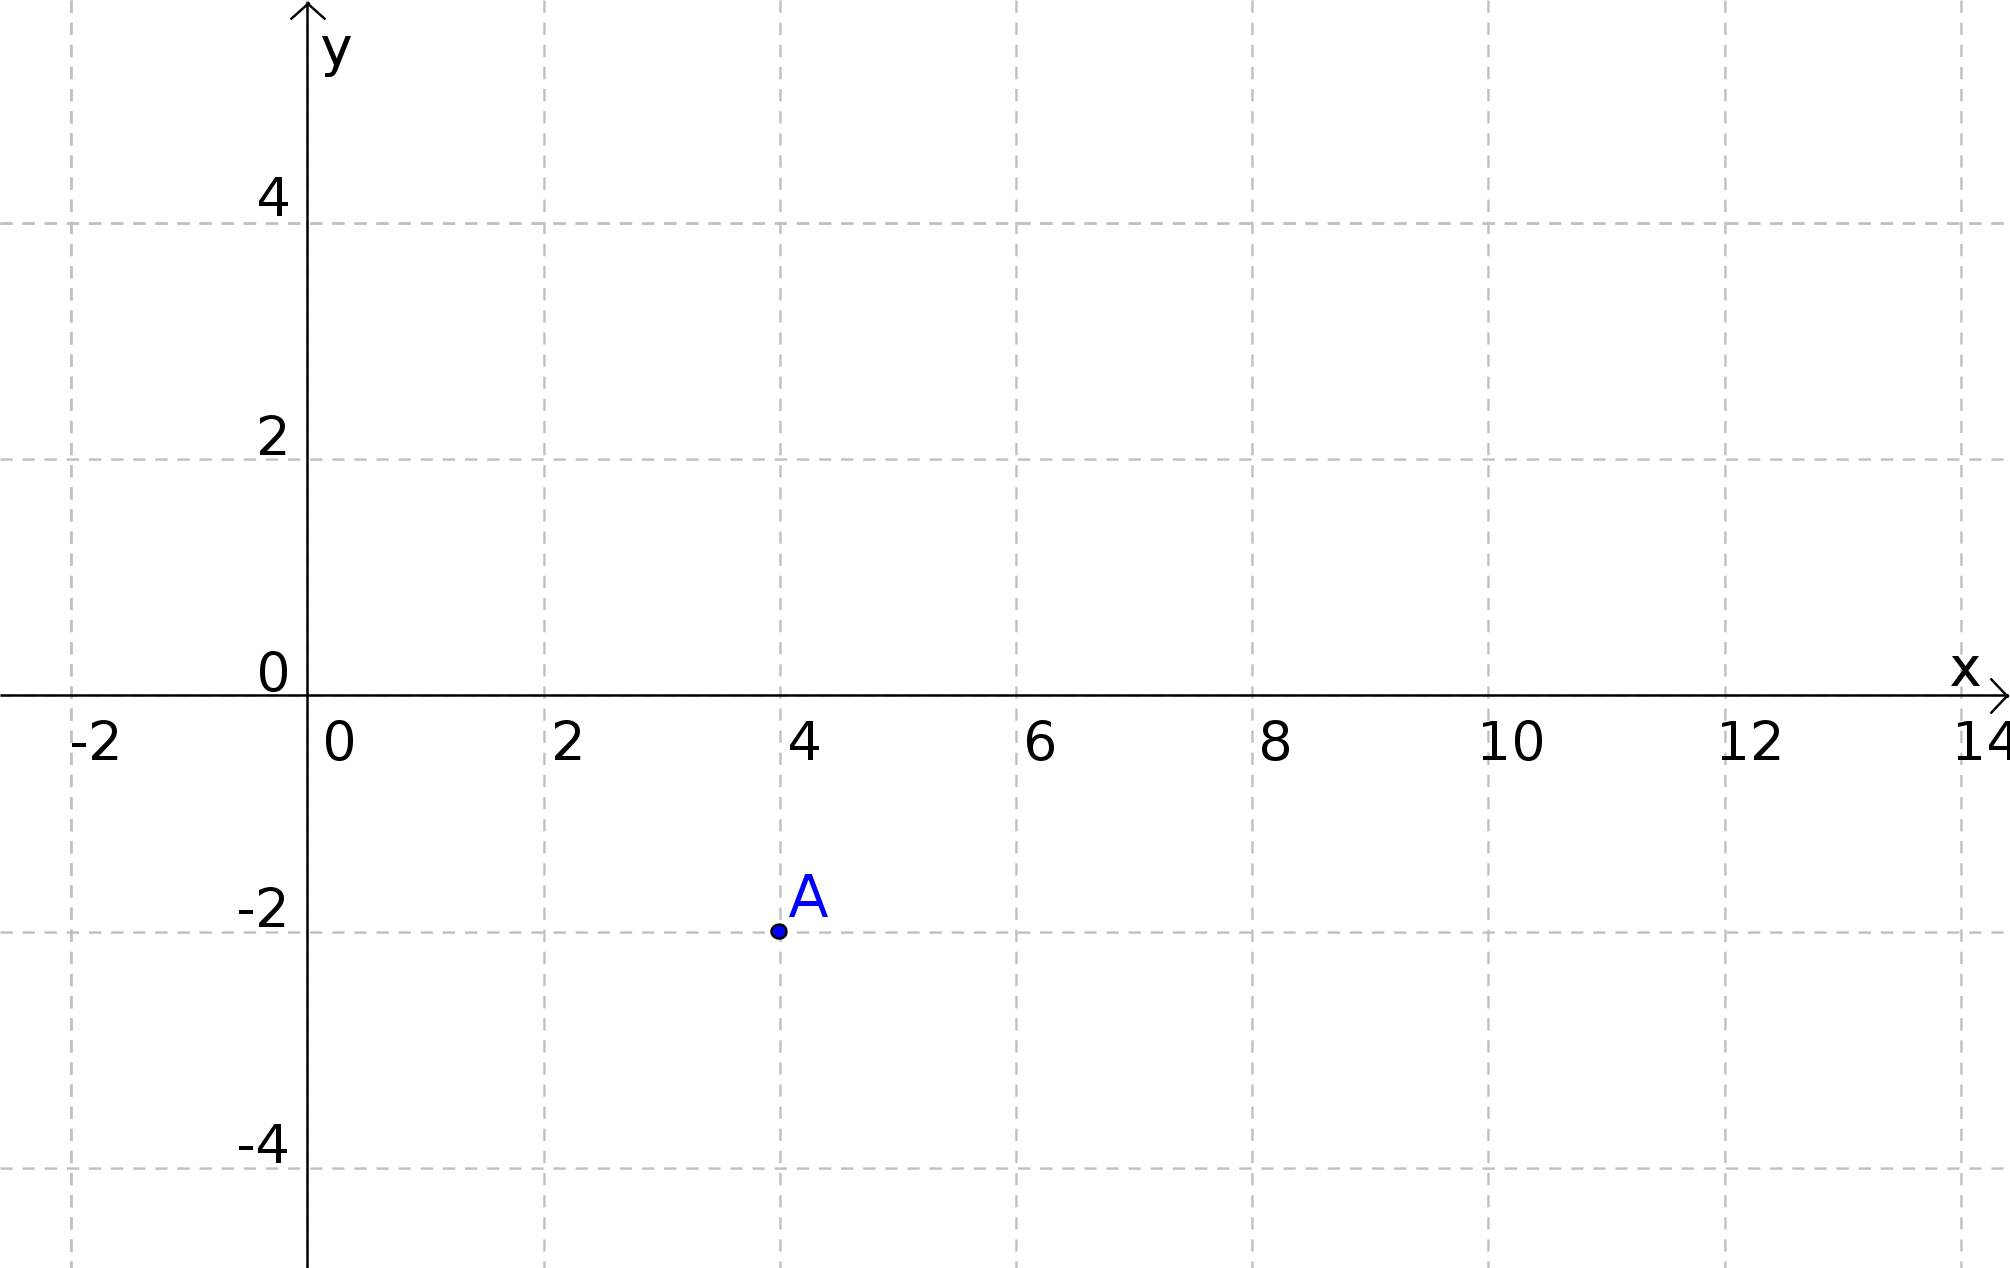
\includegraphics[width=0.5\textwidth]{Philippe/Figures_Philippe/calcul_6_5.png}
                \end{center}
            \end{question}

            \begin{reponses}
                \item[false] $(2;4)$
                \item[false] $(2;1)$
                \item[false] $(1;2)$
                \item[true] $(4;2)$
            \end{reponses}
            %%%%%%%%%%%%%%%%%%%%%%%%%%%%%%%%%%%%%
            
        \subsection{Reconnaître une situation de proportionnalité}
        	
            \begin{question}{1219}{Calcul}{1}{/}
            	6 patates permettent de nourrir 3 personnes pendant une soirée raclette. Avec 12 patates, combien de personnes est-il possible de nourrir?
            \end{question}

            \begin{reponses}
            	\item[false] 7
            	\item[true] 6
                \item[false] 5
                \item[false] 4
            \end{reponses}
			%%%%%%%%%%%%%%%%%%%%%%%%%%%%%%%%%%%%%
        	
            \begin{question}{1219}{Calcul}{2}{/}
            	6 patates permettent de nourrir 3 personnes pendant une soirée raclette. Combien de personnes peuvent nourrir $n$ patates?
            \end{question}

            \begin{reponses}
            	\item[false] $3n$
            	\item[false] $2n$
                \item[false] $n$
                \item[true] $n/2$
            \end{reponses}
			%%%%%%%%%%%%%%%%%%%%%%%%%%%%%%%%%%%%%
        	
            \begin{question}{1219}{Calcul}{2}{/}
            	Un objet est lâché sans vitesse initiale et n'est soumis qu'à son seul poids. Sa vitesse s'exprime alors comme $v(t)=gt$ avec $g$ une constante. Que vaut sa vitesse à $t=10\;\si{\second}$ sachant qu'elle valait \SI{49,05}{\meter\per\second} a $t=5\;\si{\second}$?
            \end{question}

            \begin{reponses}
            	\item[false] \SI{490,5}{\meter\per\second}
            	\item[false] \SI{981}{\meter\per\second}
                \item[false] \SI{49,05}{\meter\per\second}
                \item[true] \SI{98,1}{\meter\per\second}
            \end{reponses}
			%%%%%%%%%%%%%%%%%%%%%%%%%%%%%%%%%%%%%
        
        \subsection{Simplifier des expressions}
        
        	\begin{question}{9}{Calcul}{1}{/}
				Quelle est la simplification de l'expression $\frac{a \times b}{a \times c}$
            \end{question}

            \begin{reponses}
            	\item[false] $\frac{a^2b}{c}$
            	\item[true] $\frac{b}{c}$
                \item[false] $\frac{a^2}{bc}$
                \item[false] $\frac{ab}{c}$
            \end{reponses}
			%%%%%%%%%%%%%%%%%%%%%%%%%%%%%%%%%%%%%
        
        	\begin{question}{9}{Calcul}{2}{/}
				Quelle est la simplification de l'expression $\frac{2 \times 3}{10}$
            \end{question}

            \begin{reponses}
            	\item[true] $\frac{3}{5}$
            	\item[false] $\frac{6}{10}$
                \item[false] $\frac{5}{3}$
                \item[false] $\frac{10}{6}$
            \end{reponses}
			%%%%%%%%%%%%%%%%%%%%%%%%%%%%%%%%%%%%%
        
        	\begin{question}{9}{Calcul}{2}{/}
				Quelle est la simplification de l'expression $\frac{\sqrt{2} \times 3}{2}$
            \end{question}

            \begin{reponses}
            	\item[false] $\frac{3}{2}$
            	\item[false] $\frac{\sqrt{2}}{3}$
                \item[false] $\frac{6}{\sqrt{2}}$
                \item[true] $\frac{3}{\sqrt{2}}$
            \end{reponses}
			%%%%%%%%%%%%%%%%%%%%%%%%%%%%%%%%%%%%%
        
        	\begin{question}{9}{Calcul}{2}{/}
				Quelles sont les simplifications de l'expression $\frac{16x+ 12y}{8}$
            \end{question}

            \begin{reponses}
            	\item[false] $\frac{2x+3y}{2}$
                \item[true] $\frac{4x+3y}{2}$
            	\item[true] $2x+\frac{3y}{2}$
                \item[false] $2x+\frac{2y}{3}$
            \end{reponses}
			%%%%%%%%%%%%%%%%%%%%%%%%%%%%%%%%%%%%%
        
        \subsection{Savoir résoudre des équations algébriques d'ordre deux}
        
        	\begin{question}{1132}{Calcul}{1}{/}
				Quelles sont les solutions (ou racines) de $ax^2+bx+c=0$?
            \end{question}

            \begin{reponses}
            	\item[true] $x=\frac{-b+\sqrt{b^2-4ac}}{2a}$ et $x=\frac{-b-\sqrt{b^2-4ac}}{2a}$ si $b^2-4ac\geq 0$. Aucune solution réelle si $b^2-4ac<0$
            	\item[false] $x=\frac{-b}{2a}$ et $x=\frac{b}{2a}$ si $b^2-4ac>=0$. Aucune solution réelle si $b^2-4ac<0$
                \item[false] $x=\frac{-b+\sqrt{b^2-4ac}}{2a}$ et $x=\frac{-b-\sqrt{b^2-4ac}}{2a}$ si $b^2-4ac<0$. Aucune solution réelle si $b^2-4ac\geq 0$
                \item[false] $x=\frac{b+\sqrt{b^2-4ac}}{2a}$ et $x=\frac{b-\sqrt{b^2-4ac}}{2a}$ si $b^2-4ac>=0$. Aucune solution réelle si $b^2-4ac<0$
            \end{reponses}
			%%%%%%%%%%%%%%%%%%%%%%%%%%%%%%%%%%%%%
        
        	\begin{question}{1132}{Calcul}{2}{/}
				Quelles sont les solutions (ou racines) de $x^2-x-2=0$?
            \end{question}

            \begin{reponses}
            	\item[false] $x=1/2$ et $x=-1/2$
            	\item[true] $x=2$ et $x=-1$
                \item[false] Aucune solution réelle
                \item[false] $x=-2$ et $x=1$
            \end{reponses}
			%%%%%%%%%%%%%%%%%%%%%%%%%%%%%%%%%%%%%
        

        \subsection{Savoir trouver l'équation d'une droite à partir de deux points}
        
        	\begin{question}{27}{Calcul}{1}{1223}
				Une droite passe par les points $A = (0;0)$ et $B = (2;3)$. Quelle est son équation?
            \end{question}

            \begin{reponses}
            	\item[true] $y(x)=\frac{3}{2}x$
            	\item[false] $y(x)=\frac{2}{3}x$
                \item[false] $y(x)=\frac{3}{2}x+1$
                \item[false] $y(x)=\frac{2}{3}x+1$
            \end{reponses}
			%%%%%%%%%%%%%%%%%%%%%%%%%%%%%%%%%%%%%

            \begin{question}{27}{Calcul}{2}{1223}
                Une droite passe par les points $A = (1;2)$ et $B = (5;7)$. Quelle est son équation?
            \end{question}

            \begin{reponses}
                \item[false] $y(x)=\num{0.8}x+\num{1.2}$
                \item[true] $y(x)=\num{1.25}x+\num{0.75}$
                \item[false] $y(x)=\num{0.75}x+\num{1.25}$
                \item[false] $y(x)=\num{1.2}x+\num{0.8}$
            \end{reponses}
            %%%%%%%%%%%%%%%%%%%%%%%%%%%%%%%%%%%%%

            \begin{question}{27}{Calcul}{2}{1223}
                Quelle est l'équation de la droite $AB$?\\
                \begin{center}
                	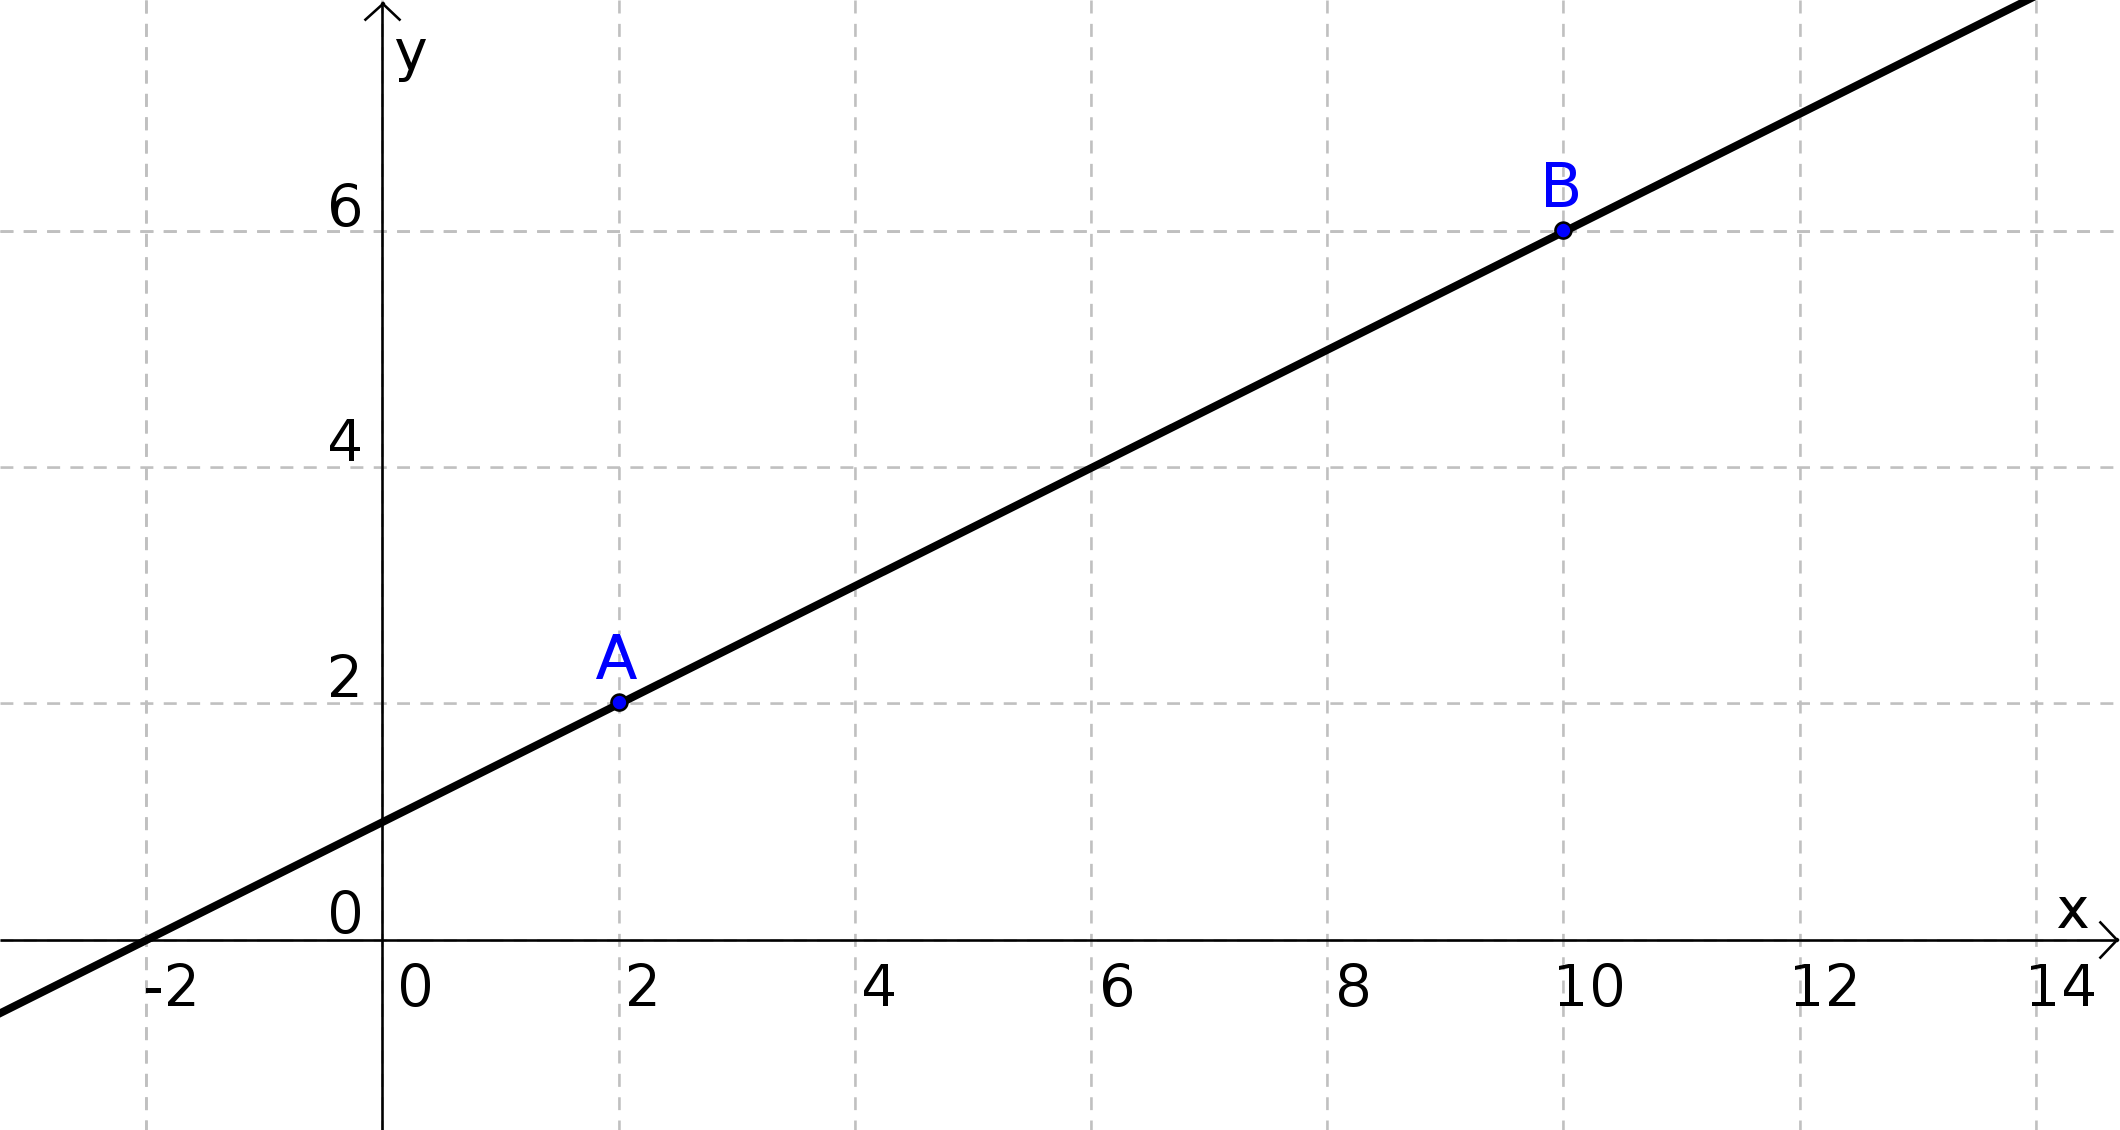
\includegraphics[width=0.5\textwidth]{Philippe/Figures_Philippe/calcul_6_9.png}
                \end{center}
            \end{question}

            \begin{reponses}
                \item[true] $y(x)=1/2x+1/2$
                \item[false] $y(x)=-2x+1/2$
                \item[false] $y(x)=1/2x-2$
                \item[false] $y(x)=x-1/2$
            \end{reponses}
            %%%%%%%%%%%%%%%%%%%%%%%%%%%%%%%%%%%%%

            \begin{question}{27}{Calcul}{2}{1223}
                En mesurant la vitesse d'un objet en chute libre à un temps $t=\SI{1}{\second}$ et $t=\SI{5}{\second}$, on trouve respectivement \SI{12}{\meter\per\second} et \SI{52}{\meter\per\second}. On sait que la vitesse d'un objet en chute libre dépend linéairement du temps (\textit{i.e.} $v(t) = a.t+b$). Que valent $a$ et $b$ dans ce cas?
            \end{question}

            \begin{reponses}
                \item[false] $a=2$ et $b=10$.
                \item[true] $a=10$ et $b=2$.
                \item[false] $a=8$ et $b=12$.
                \item[false] $a=12$ et $b=8$.
            \end{reponses}
            %%%%%%%%%%%%%%%%%%%%%%%%%%%%%%%%%%%%%

        \subsection{Dans les situations de proportionnalité, trouver une valeur manquante en utilisant une règle de 3}

            \begin{question}{1215}{Calcul}{1}{1219}
                On donne $8\times x=4$. Que vaut $x$?
            \end{question}

            \begin{reponses}
                \item[true] 0,5
                \item[false] 2
                \item[false] 12
                \item[false] 4
            \end{reponses}
            %%%%%%%%%%%%%%%%%%%%%%%%%%%%%%%%%%%%%
        
        	\begin{question}{1215}{Calcul}{2}{1219}
				On donne $\sqrt{2} \times \frac{x}{3}=1$. Que vaut $x$?
            \end{question}

            \begin{reponses}
            	\item[false] $\frac{\sqrt{2}}{3}$
            	\item[false] $1-\frac{3}{\sqrt{2}}$
                \item[false] $1-\frac{\sqrt{2}}{3}$
                \item[true] $\frac{3}{\sqrt{2}}$
            \end{reponses}
			%%%%%%%%%%%%%%%%%%%%%%%%%%%%%%%%%%%%%

            \begin{question}{1215}{Calcul}{2}{1219}
                La force de rappel d'un ressort est égal à $-k\Delta x$, avec $k$ la constante de rappel et $\Delta x$ la position de l'extrémité du ressort par rapport à la position d'équilibre. On mesure une force de \SI{-4}{\newton} et un écart à l'équilibre de $\Delta x=$\SI{0,05}{\meter}. Quelle est la valeur de $k$?
            \end{question}

            \begin{reponses}
                \item[false] \SI{0,0125}{\newton\per\meter}
                \item[true] \SI{80}{\newton\per\meter}
                \item[false] \SI{0,2}{\newton\per\meter}
                \item[false] \SI{10}{\newton\per\meter}
            \end{reponses}
            %%%%%%%%%%%%%%%%%%%%%%%%%%%%%%%%%%%%%
        
        \subsection{Utiliser la notation scientifique en recourant aux puissances de 10 + Calculer à la main la puissance de 10 d'une application numérique}

            \begin{question}{/}{Calcul}{2}{1210 et 1211}
                Que vaut $(\num{0.4} \times 120)/\num{0.3}$?
            \end{question}

            \begin{reponses}
                \item[true] \num{1.6e2}
                \item[false] \num{1.6e-2}
                \item[false] \num{1.6e1}
                \item[false] \num{1.6e-1}
            \end{reponses}
            %%%%%%%%%%%%%%%%%%%%%%%%%%%%%%%%%%%%%

            \begin{question}{/}{Calcul}{2}{1210 et 1211}
                On étudie un gaz parfait de volume $V=\SI{0.02}{\meter\cubed}$, de température $T=\SI{300}{\kelvin}$ et de quantité de matière $n=\SI{0.5}{\mole}$. Sachant que $P=nRT/V$ et que $R\simeq\SI{8}{\joule\per\mole\per\kelvin}$, la pression $P$ du gaz est:
            \end{question}

            \begin{reponses}
                \item[true] \SI{6e4}{\pascal}
                \item[false] \SI{6}{\pascal}
                \item[false] \SI{6e3}{\pascal}
                \item[false] \SI{6e1}{\pascal}
            \end{reponses}
            %%%%%%%%%%%%%%%%%%%%%%%%%%%%%%%%%%%%%
        
        	\begin{question}{/}{Calcul}{3}{1210 et 1211}
				Que vaut $\left(0,003 \times 40 \times 10^3 \times 5 \times 10^{-2} \right)/\left(0,6 \times 10^{1} \right) $?
            \end{question}

            \begin{reponses}
            	\item[false] 20
            	\item[false] 2
                \item[false] 10
                \item[true] 1
            \end{reponses}
			%%%%%%%%%%%%%%%%%%%%%%%%%%%%%%%%%%%%%

            \begin{question}{/}{Calcul}{3}{1210 et 1211}
                Le principe d'incertitude de Heisenberg énonce qu'il n'est jamais possible de connaître avec une infinie précision à la fois la position et l'impulsion d'un objet. L'équation qui décrit ce principe s'écrit $\sigma_x \times \sigma_p > \frac{\hbar}{2}$, où $\sigma_x$ et $\sigma_p$ sont les incertitudes sur la position et l'impulsion, respectivement, et $\hbar = \frac{h}{2\pi} \simeq \SI{1,7e-34}{\joule\second}$ est la constante de Planck réduite. Calculer l'incertitude minimum $\sigma_x$ dans le cas d'un humain dont l'impulsion est connue à $\pm \SI{5e-2}{\kilo\gram\meter\per\second}$ près.
            \end{question}

            \begin{reponses}
                \item[false] \SI{8,5e-35}{\meter}
                \item[true] \SI{1,7 e-33}{\meter}
                \item[false] \SI{8,5e-34}{\meter}
                \item[false] \SI{1,7e-32}{\meter}
            \end{reponses}
            %%%%%%%%%%%%%%%%%%%%%%%%%%%%%%%%%%%%%
            
        \subsection{Savoir résoudre des équations algébriques d'ordre un}
        
        	\begin{question}{8}{Calcul}{1}{1215}
				Quelle est la solution de $a.x+b=c$?
            \end{question}

            \begin{reponses}
            	\item[false] $x=c-b-a$
            	\item[false] $x=\frac{c}{a}-b$
                \item[true] $x=\frac{c-b}{a}$
                \item[false] $x=(c+b)/a$
            \end{reponses}
			%%%%%%%%%%%%%%%%%%%%%%%%%%%%%%%%%%%%%
        
        	\begin{question}{8}{Calcul}{1}{1215}
				Quelle est la solution de $3x+2=4$?
            \end{question}

            \begin{reponses}
            	\item[false] $x=-1$
            	\item[false] $x=\frac{4}{3}-2$
                \item[true] $x=\frac{2}{3}$
                \item[false] $x=2$
            \end{reponses}
			%%%%%%%%%%%%%%%%%%%%%%%%%%%%%%%%%%%%%

        \subsection{Trouver une valeur manquante en utilisant des pourcentages}
        
        	\begin{question}{1216}{Calcul}{1}{1215}
				Que vaut $x$ pourcent de $y$?
            \end{question}

            \begin{reponses}
            	\item[false] $y\times x$
            	\item[true] $y\times \frac{x}{100}$
                \item[false] $\frac{y}{100x}$
                \item[false] $100y/x$
            \end{reponses}
			%%%%%%%%%%%%%%%%%%%%%%%%%%%%%%%%%%%%%
        
        	\begin{question}{1216}{Calcul}{1}{1215}
				Que vaut $y$ augmenté de $x$ pourcent?
            \end{question}

            \begin{reponses}
            	\item[false] $y\times (1+x)$
            	\item[false] $y\times \frac{x}{100}$
                \item[true] $y\times (1+\frac{x}{100})$
                \item[false] $101y/x$
            \end{reponses}
			%%%%%%%%%%%%%%%%%%%%%%%%%%%%%%%%%%%%%

            \begin{question}{1216}{Calcul}{2}{1215}
                Un article coûte, hors soldes, 60 euros. Son coût diminue de \SI{30}{\percent} durant les soldes. Combien coûte-t-il durant les soldes?
            \end{question}

            \begin{reponses}
                \item[false] 20 euros
                \item[false] 18 euros
                \item[true] 42 euros
                \item[false] 40 euros
            \end{reponses}
            %%%%%%%%%%%%%%%%%%%%%%%%%%%%%%%%%%%%%

            \begin{question}{1216}{Calcul}{2}{1215}
                On mesure l'activité d'une source radioactive et on trouve \SI{120}{\becquerel}. On mesure la même source un jour plus tard, et on trouve qu'elle a diminué de \SI{60}{\percent}. Que vaut cette nouvelle activité?
            \end{question}

            \begin{reponses}
                \item[false] \SI{72}{\becquerel}
                \item[true] \SI{48}{\becquerel}
                \item[false] \SI{20}{\becquerel}
                \item[false] \SI{100}{\becquerel}
            \end{reponses}
            %%%%%%%%%%%%%%%%%%%%%%%%%%%%%%%%%%%%%
        
        \subsection{Savoir résoudre des équations algébriques d'ordre deux + simplifier des expressions}

            \begin{question}{/}{Calcul}{2}{1132 et 9}
                Quelles sont les racines du polynôme $-9x^2+3x+2$?
            \end{question}

            \begin{reponses}
                \item[true] $\frac{1\pm 3}{6}$
                \item[false] $\frac{3 \pm 1}{6}$
                \item[false] $\frac{-3 \pm 1}{6}$
                \item[false] $\frac{-1 \pm 3}{6}$
            \end{reponses}
            %%%%%%%%%%%%%%%%%%%%%%%%%%%%%%%%%%%%%

            \begin{question}{/}{Calcul}{2}{1132 et 9}
                Un boulet de canon suit un trajectoire parabolique qui a pour équation $z(t)=-\frac{1}{2}gt^2+v_0t+z_0$. En supposant que $z_0 = \SI{3.0}{\meter}$ et $v_0 = \SI{2.0}{\meter\per\second}$, à quelle instant $t$ le boulet va-t-il toucher le sol? (On approxime $g\simeq\SI{10}{\meter\per\second\squared}$)
            \end{question}

            \begin{reponses}
                \item[false] \SI{0.6}{\second}
                \item[false] \SI{2}{\second}
                \item[false] \SI{1.2}{\second}
                \item[true] \SI{1}{\second}
            \end{reponses}
            %%%%%%%%%%%%%%%%%%%%%%%%%%%%%%%%%%%%%
        
        	\begin{question}{/}{Calcul}{3}{1132 et 9}
				Pour quelles valeurs de $x$ non-nul l'expression $3\pi x^2 + 2x + \sqrt{2}x^3$ est-elle nulle?
            \end{question}

            \begin{reponses}
            	\item[false] Il n'y a pas de solutions réelles
            	\item[true] $\frac{-3\pi \pm \sqrt{9\pi^2-8\sqrt{2}}}{2\sqrt{2}}$
                \item[false] $\frac{3\pi \pm \sqrt{9\pi^2-8\sqrt{2}}}{2\sqrt{2}}$
                \item[false] $\frac{-3\pi \pm \sqrt{9\pi^2+8\sqrt{2}}}{2\sqrt{2}}$
            \end{reponses}
			%%%%%%%%%%%%%%%%%%%%%%%%%%%%%%%%%%%%%

    \section{Fonctions usuelles}

        \subsection{Connaître les différentes propriétés des fonctions usuelles}
        
        	\begin{question}{30}{Fonctions usuelles}{1}{/}
				Lesquelles de ces affirmations sont vraies?
            \end{question}

            \begin{reponses}
            	\item[true] $\lim_{x\to +\infty} e^x = +\infty$
            	\item[true] $\lim_{x\to -\infty} e^x = 0$
                \item[true] $\lim_{x\to 0} \ln (x) = -\infty$
                \item[true] $\lim_{x\to +\infty} 1/(x) = 0$
            \end{reponses}
			%%%%%%%%%%%%%%%%%%%%%%%%%%%%%%%%%%%%%

            \begin{question}{30}{Fonctions usuelles}{2}{/}
                Quelle affirmation est vraie à propos de la fonction $f(x)=3e^{-x}$? (plusieurs réponses possibles)
            \end{question}

            \begin{reponses}
                \item[true] Elle est décroissante.
                \item[false] Elle vaut 1 quand $x=0$.
                \item[true] Elle est positive.
                \item[false] Elle est croissante.
            \end{reponses}
			%%%%%%%%%%%%%%%%%%%%%%%%%%%%%%%%%%%%%

            \begin{question}{30}{Fonctions usuelles}{2}{/}
                L'activité d'une source radioactive suit une loi qui s'écrit $A(t)=A_0 e^{-\lambda t}$, avec $A_0 > 0$. Quelle affirmation est vraie à propos de cette loi? (plusieurs réponses possibles)
            \end{question}

            \begin{reponses}
                \item[false] Elle est négative.
                \item[true] Elle vaut $A_0$ quand $t=0$.
                \item[true] Elle est positive.
                \item[false] Elle est croissante.
            \end{reponses}
            %%%%%%%%%%%%%%%%%%%%%%%%%%%%%%%%%%%%%
	
    \section{Modélisation}
    
    	\subsection{Connaître les dimensions des grandeurs physique usuelles}
        	
            \begin{question}{1225}{Modélisation}{1}{/}
				Quelle est l'unité usuelle d'une longueur? 
            \end{question}

            \begin{reponses}
            	\item[false] \si{\kilo\gram}
            	\item[true] \si{\meter}
                \item[false] \si{\ampere}
                \item[false] \si{\second}
            \end{reponses}
			%%%%%%%%%%%%%%%%%%%%%%%%%%%%%%%%%%%%%
        	
            \begin{question}{1225}{Modélisation}{1}{/}
				Quelle est l'unité usuelle d'une vitesse? 
            \end{question}

            \begin{reponses}
            	\item[true] \si{\meter\per\second}
            	\item[false] \si{\kilo\gram\per\meter}
                \item[false] \si{\gram\per\second}
                \item[false] \si{\second}
            \end{reponses}
			%%%%%%%%%%%%%%%%%%%%%%%%%%%%%%%%%%%%%
        	
            \begin{question}{1225}{Modélisation}{1}{/}
				Quelle est l'unité usuelle d'une accélération? 
            \end{question}

            \begin{reponses}
                \item[false] \si{\gram\per\second^2}
            	\item[true] \si{\meter\per\second^2}
                \item[false] \si{\second^2}
            	\item[false] \si{\kilo\gram\per\meter^2}
            \end{reponses}
			%%%%%%%%%%%%%%%%%%%%%%%%%%%%%%%%%%%%%
        	
            \begin{question}{1225}{Modélisation}{2}{/}
				Quelle est l'unité d'une force, sachant qu'une force a la même unité qu'une masse multipliée par une accélération?
            \end{question}

            \begin{reponses}
            	\item[true] \si{\kilo\gram.\meter\per\second^2}
            	\item[false] \si{\kilo\gram\per\meter\per\second}
                \item[false] \si{\gram\per\second}
                \item[false] \si{\kilo\gram\per\second}
            \end{reponses}
			%%%%%%%%%%%%%%%%%%%%%%%%%%%%%%%%%%%%%
    	
        \subsection{Vérifier un résultat par analyse dimensionnelle}
        
        	\begin{question}{1226}{Modélisation}{2}{non créé}
				Lors d'un examen, un étudiant doit calculer l'expression de la vitesse d'un objet. Laquelle de ces formules peut être correcte? ($g=\SI{9,81}{\meter\per\second^20}$, $t$ est un temps, $d$ une distance, $m$ une masse).
            \end{question}

            \begin{reponses}
            	\item[false] $\frac{gt}{d}$
            	\item[true] $gt$
                \item[false] $\frac{d}{gt}$
                \item[false] $gd$
            \end{reponses}
			%%%%%%%%%%%%%%%%%%%%%%%%%%%%%%%%%%%%%

            \begin{question}{1226}{Modélisation}{2}{non créé}
				Lors d'un examen, un étudiant doit calculer l'expression de l'énergie cinétique d'un objet. Une réponse est correcte, laquelle? ($g=\SI{9,81}{\meter\per\second^20}$, $t$ est un temps, $d$ une distance, $m$ une masse).
            \end{question}

            \begin{reponses}
                \item[false] $\frac{1}{2}mgt$
                \item[false] $\frac{1}{2}mgdt^2$
                \item[true] $\frac{1}{2}mg^2t^2$
                \item[false] $\frac{1}{2}mg^2d^2$
            \end{reponses}
			%%%%%%%%%%%%%%%%%%%%%%%%%%%%%%%%%%%%%
        
        	\begin{question}{1226}{Modélisation}{3}{non créé}
				A quelle grandeur physique peut correspondre $\gamma m v^2$ sachant que $m$ est une masse, $v$ une vitesse, et que $\gamma=\frac{1}{\sqrt{1-\frac{v^2}{c^2}}}$, avec $c$ la vitesse de la lumière?
            \end{question}

            \begin{reponses}
            	\item[false] une quantité de mouvement
            	\item[false] une force
                \item[false] une vitesse
                \item[true] une énergie
            \end{reponses}
			%%%%%%%%%%%%%%%%%%%%%%%%%%%%%%%%%%%%%
    	

\end{document}
